
\documentclass[12pt]{book}
\usepackage[b5paper,right=40mm]{geometry}                % See geometry.pdf to learn the layout options.
%\usepackage[paperwidth=9.2cm, paperheight=12.4cm, width=9cm, height=12cm,top=0.2cm,bottom=0.4cm,left=0.2cm,right=0.2cm,foot=0cm]{geometry}
%\geometry{landscape}                % Activate for for rotated page geometry
%\usepackage[parfill]{parskip}    % Activate to begin paragraphs with an empty line rather than an indent
\usepackage{graphicx}
\graphicspath{{graphics/new/}}
\usepackage{amssymb}
\usepackage{framed}
\usepackage{ragged2e}
\usepackage{changepage}
\usepackage{paralist}
\usepackage{textcase}
\usepackage{setspace}
\usepackage{natbib}
%\usepacakge{optparams}
\usepackage{placeins}
\usepackage{titlesec}
\usepackage{titletoc}
\usepackage{marginnote}
\usepackage{caption}
\renewcommand*{\marginfont}{\color{cyan}\scriptsize}
\renewcommand*{\raggedleftmarginnote}{}
\usepackage[pdfstartview=FitH,
            bookmarksnumbered=true,
            bookmarksopen=true,
            colorlinks=true,
            pdfborder={0 0 1},
            citecolor=blue,
            linkcolor=cyan,
            anchorcolor=green,
            urlcolor=blue,
            breaklinks=true,]{hyperref}

%\usepackage{caption}
\usepackage{xifthen}
\usepackage{bm}
\usepackage{exercise}
\usepackage{amsbsy}
%\usepackage{fontspec,xltxtra,xunicode}
\usepackage{amsmath}
\usepackage{pstricks}


\def\um{\mathrm{um}}
\def\mm{\mathrm{mm}}
\def\m{\mathrm{m}}
\def\s{\mathrm{s}}
\let\sb=_ \catcode`\_=\active \def_#1{\ensuremath \sb{\rm#1}}

\title{Optical Properties of Solids}
\author{MARK FOX}
\date{}                                           % Activate to display a given date or no date

\makeatletter
  \newcommand\figcaption{\def\@captype{figure}\caption}
  \newcommand\tabcaption{\def\@captype{table}\caption}
\long\def\@makecaption#1#2{
   \vskip\abovecaptionskip
   \sbox\@tempboxa{\centering\fontsize{10pt}{#1\qquad #2} }
   \ifdim \wd\@tempboxa >\hsize
     \centering\fontsize{10pt}{#1\qquad #2} \par
   \else
     \global \@minipagefalse
     \hb@xt@\hsize{\hfil\box\@tempboxa\hfil}
   \fi
   \vskip\belowcaptionskip}
\makeatother

\begin{document}
\pagestyle{empty}
\psset{unit=1in}
\begin{pspicture}(4,5)% use your page size
  \rput[b](2.5,2){\parbox{3in}
  {\begin{flushright}
    \Huge\bfseries\sffamily{Optical Properties of \\ Solids}
    \end{flushright}}}

  \uput[-90](2.5,3.3){\color{red}\rule{4in}{1ex}}
  \uput[0](4.2,2){\color{red}\rule{1.6ex}{6in}}
\end{pspicture}

%\maketitle
\tableofcontents
\chapter{Introduction}\label{chap:1}

\setcounter{page}{1}

\definecolor{shadecolor}{rgb}{0.9,0.9,0.9}
\begin{shaded}

Light interacts with matters in many different ways. Metals are shiny, but water is transparent. Strained glass and gemstones transmit some colors, but absorb others. Other materials such as milk appear white because they scatter the incoming light in all directions.

In the chapters that follow, we will be looking at a whole host of these optical phenomena in a wide range of solid state materials. Before we can begin to do this, we must first describe the way in which the phenomena are classified, and the coefficients that used to quantify them. We must then introduce the materials that we will be studying, and clarify in general terms how the solid state is different from the gas and liquid phase. This is the subject of the present chapter.
\end{shaded}


\section{Classification of Optical Processes}\label{sec:1.1}

The wide-ranging optical properties observed in solid state materials can be classified into a small number of general phenomena. The simplest group, namely \textbf{reflection}, \textbf{propagation} and \textbf{transmission}, is illustrated in Fig \ref{fig:1.1}. This shows a light beam incident on an optical medium. Some of the light is reflected from the front surface, while the rest enters the medium and propagates through if. If any of this light reaches the back surface, it can be reflected again, or it can be transmitted through to the other side. The amount of light transmitted is therefore related to the reflectivity at the front and back surfaces and also to the way the light propagates through the medium.


The phenomena that can occur while light propagates through an optical medium are illustrated schematically in Fig \ref{fig:sche}.

\begin{figure}[http]
\begin{center}\label{fig:sche}
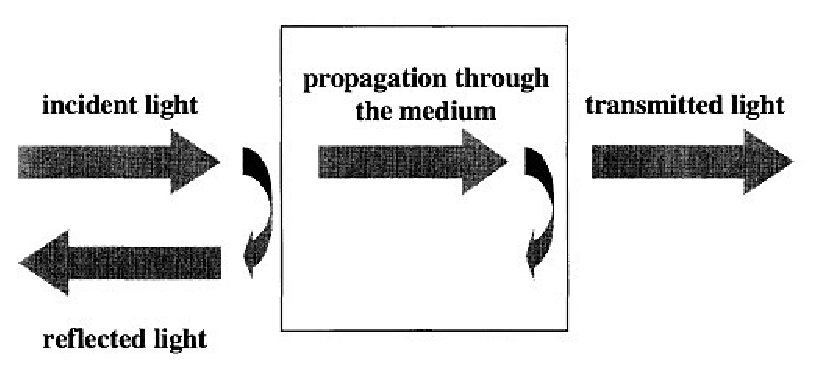
\includegraphics[width=0.8\textwidth]{11.eps}
\end{center}
\end{figure}
\vspace{-3\baselineskip}

\marginnote{Fig. \ref{fig:1.1}Reflection, propagation and transmission of a light beam incident on an optical medium.}

\vspace{2\baselineskip}
\begin{description}
\item[Refraction] causes the light waves to propagate with a smaller velocity than in free space. This reduction of the velocity leads to the bending of light rays at interfaces described by Snell's law of refraction. Refraction, in itself, does not affect the intensity of the light wave as it propagates.
\item[Absorption] occurs during the propagation if the frequency of the light is resonant  with the transition frequencies of the atoms in the medium. In this case, the beam will be attenuated as it progresses. The transmission of the medium is clearly related to the absorption, because only unabsorbed light will be transmitted. Selective absorption is responsible for the coloration of many optical materials. Rubies, for example, are red because they absorb blue and green light, but not red.
\item[Luminescence] is  the general name given to the process of spontaneous emission of light by excited atoms in a solid state material. One of the ways in which the atoms can be promoted into excited states prior to spontaneous emission is by the absorption of light. Luminescence can thus accompany the propagation of light in an absorbing medium. The light is emitted in all directions, and has a different frequency to the incoming beam.

Luminescence does not always have to accompany absorption. It takes a characteristic amount of time for the excited atoms to re-emit by spontaneous emission. This means that it might be possible for the excited atoms to dissipate the excitation energy as heat before the radiative re-emission process occurs. The efficiency of the luminescence process is therefore closely tied up with the dynamics of the de-excitation mechanisms in the atoms.\marginnote{
\begin{minipage}{\textwidth}
    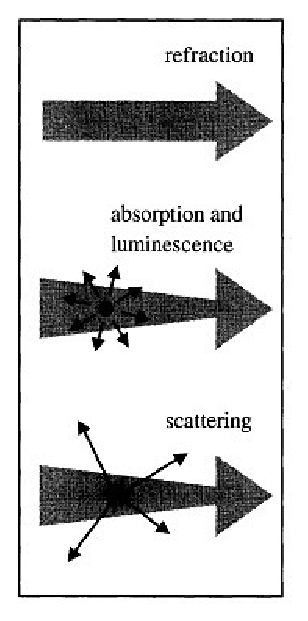
\includegraphics[height=50mm]{12.eps}
    \label{fig:1.2}
  \end{minipage}
 \\ [\intextsep]
Fig. \ref{fig:1.2}Phenomena that can occur as a light beam propagates through an optical medium. Refraction causes a reduction in the velocity of the wave, while absorption causes attenuation. Luminescence can accompany absorption if the excited atoms re-emit by spontaneous emission. Scattering causes a redirection of the light. The diminishing width of the arrow for the processes of absorption and scattering represents the attenuation of the beam. }

\item[Scattering] is the phenomenon in which the light changes direction and possibly also its frequency after interacting with the medium. The total number of photons is unchanged, but the number going in the forward direction decreases because light is being re-directed in other directions. Scattering therefore has the same attenuating effect as absorption. The scattering is said to be elastic if the frequency of the scattered light is unchanged, or inelastic if the frequency changes in the process. The difference in the photon energy in an inelastic scattering process has to be taken from the medium if the frequency increases or given to the medium if the frequency decreases.
\end{description}


A number of other phenomena can occur as the light propagates through the medium if the intensity of the beam is very high. These are described by \textbf{nonlinear optics}. An example is frequency doubling, in which the frequency of part of a beam is doubled by interaction with the optical medium. These nonlinear effects have only been discovered through the use of laser. At this stage, we only mention their existence for completeness, and postpone their further discussion until Chapter \ref{chap:11}.

\section{Optical Coefficients}

The optical phenomena described in the previous section can be quantified by a number of parameters that determine the properties of the medium at the macroscopic level.
The reflection at the surfaces is described by the \textbf{coefficient of reflection} or \textbf{reflectivity}. This is usually given the symbol $R$ and is defined as the ratio of the reflected power to the power incident on the surface. The \textbf{coefficient of transmission} or \textbf{transmissivity} $T$ is defined likewise as the ratio of the transmitted power to the incident power. If there is no absorption or scattering, then by conservation of energy we must have that:
\begin{equation}\label{equa:1.1}
  R+T=1
\end{equation}

The propagation of the beam through a transparent medium is described by the \textbf{refractive index} $n$. This is defined as the ratio of the velocity of light in free space $c$ to the velocity of light in the medium $v$ according to:
\begin{equation}\label{equa:1.2}
  n=\frac{c}{v}
\end{equation}

The refractive index depends on the frequency of the light beam. This effect is called \textbf{dispersion}, and will be discussed in detail in Section 2.3. In colourless transparent materials such as glass, the dispersion is small in the visible spectral region, and it therefore makes sense to speak of 'the' refractive index of the substance in question.

The absorption of light by an optical medium is quantified by its \textbf{absorption coefficient} $\alpha$. This is defined as the fraction of the power absorbed in a unit length of the medium. If the beam is propagating in the $z$ direction, and the intensity (optical power per unit area) at position $z$ is $I(z)$, then the decrease of the intensity in an incremental slice of thickness $dz$ is given by:
\begin{equation}\label{equa:1.3}
  dI=-\alpha dz\times I(z)
\end{equation}
This can be integrated to obtain \textbf{Beer's law}:
\begin{equation}\label{equa:1.4}
  I(z)=I_0e^{-\alpha z}
\end{equation}

where $I_0$ is the optical intensity at $z = 0$. The absorption coefficient is a strong function of frequency, so that optical materials may absorb one colour but not
another.

\marginnote{Equation (1.5) ignores the possibility of multiple reflections between the front and back surfaces. These will have to be included if the surfaces are parallel and the reflection coefficients are sufficiently large. We will come across some examples where these effects are important when we consider semiconductor laser diodes in Section 5.4.3 and optical bistability in Section 11.4.3. In many cases, however. the effects are small enough to be neglected, as shown in Exercises 1.8 and 1.9.}

In the next section we will explain how both the absorption and the refraction can be incorporated into a single quantity called the complex refractive index. Knowledge of this quantity enables us to calculate the reflectivity $R$, and hence the transmissivity $T$. This last point follows because the transmissivity of an absorbing medium of thickness $l$ is given by:
\begin{equation}\label{equa:1.5}
  T=(1-R_1)e^{-\alpha l}(1-R_2)
\end{equation}
where $R_1$ and $R_2$ are the reflectivities of the front and back surfaces respectively. This formula applies to the transmission of light through an optical medium such as the one shown in Fig. 1.1. The first and third terms on the right hand side of eqn \ref{equa:1.5} account for the transmission of the front and back surfaces respectively, while the middle term gives the exponential decrease in intensity due to the absorption according to Beer's law. If the front and back surfaces have equal reftectivities R, as will usually be the case, then eqn \ref{equa:1.5} simplifies to:
\begin{equation}\label{equa:1.6}
  T=(1-R)^2e^{-\alpha l}.
\end{equation}

The absorption of an optical medium can also be sometimes quantified in terms of the optical density (O.D.). This is sometimes called the \textbf{absorbance}, and is defined as:
\begin{equation}\label{equa:1.7}
  \mathrm{O.D.}=-\log_{10}\left(\frac{I(l)}{I_0}\right)
\end{equation}
\marginnote{The optical density, and hence the absorption coefficient, is usually worked out from the measured transmissivity of the sample. This requires accurate normalization of the reflection losses at the surfaces. }

where $l$ is the length of the absorbing medium. It is apparent from eqn \ref{equa:1.4} that the optical density is directly related to the absorption coefficient $\alpha$ through:
\begin{equation}\label{equa:1.8}
  \mathrm{O.D.}=\frac{\alpha l}{\log_e(10)}=0.434\alpha l
\end{equation}
In this book we will quantify the absorption by $\alpha$ instead of the optical density because it is independent of the sample length.

The phenomenon of luminescence was studied extensively by George Stokes in the nineteenth century before the advent of quantum theory. Stokes discovered that the luminescence is down-shifted in frequency relative to the absorption, an effect now known as the \textbf{Stokes shift}. Luminescence cannot be described easily by macroscopic classical parameters because spontaneous emission is fundamentally a quantum process (see Appendix B).
\marginnote{
\begin{minipage}{\textwidth}
\vspace{5\baselineskip}
    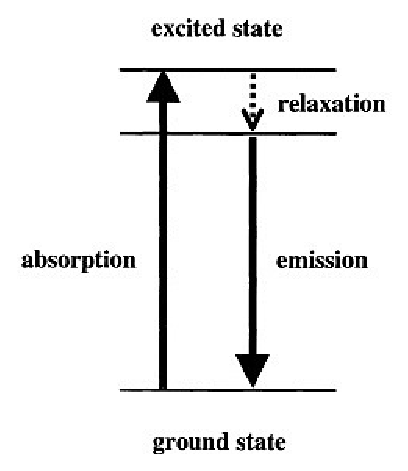
\includegraphics[height=50mm]{13.eps}
    \label{fig:1.3}
  \end{minipage}
 \\ [\intextsep]
Fig. \ref{fig:1.3} Luminescence procession an atom. The atom jumps to an excited state by absorption of a photon, then relaxed to an intermediate state, before re-emitting a photon by spontaneous emission as it falls back to the ground state. The photon emitted has a smaller energy than the absorbed photon. This reduction in the photon energy is called the Stokes Shift.}

The simplest sequence of events that takes place in luminescence is illustrated in Fig. 1.3. The atom jumps to an excited state by absorbing a photon, then relaxes to an intermediate state, and finally re-emits a photon as it drops back to the ground state. The Stokes shift is explained by applying the law of conservation of energy to the process. It is easy to see that the energy of the photon emitted must be less than that of the photon absorbed, and hence that the frequency of the emitted light is less than that of the absorbed light. The magnitude of the Stokes shift is therefore determined by the energy levels of the atoms in the medium.

\marginnote{
\begin{minipage}{\textwidth}
    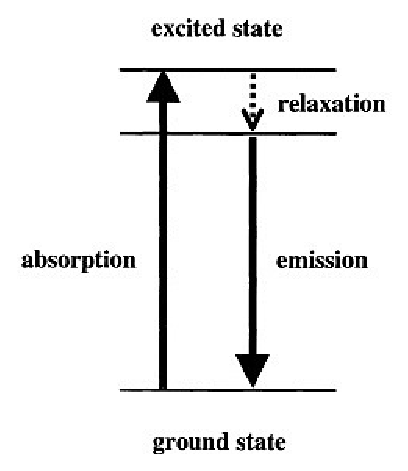
\includegraphics[height=25mm]{13.eps}
    \label{fig:1.3}
  \end{minipage}
 \\ [\intextsep]
 Luminescence process in an atom. The atom jumps to an excited state by absorption of a photon, then relaxes to an intermediate state, before re-emitting a photon by spontaneous emission as it falls back to the ground state. The photon emitted has a smaller energy than the absorbed photon. This reduction in the photon energy is called the Stokes shift.}

Scattering is caused by variations of the refractive index of the medium on a length scale smaller than the wavelength of the light. This could be caused by the presence of impurities, defects, or inhomogeneities. Scattering causes attenuation of a light beam in an analogous way to absorption. The intensity decreases exponentially as it propagates into the medium according to:
\begin{equation}\label{equa:1.9}
  I(z)=I_0\exp(-N\sigma_sz)
\end{equation}
where $N$ is the number of scattering centres per unit volume, and $\sigma_s$ is the \textbf{scattering cross-section} of the scattering centre. This is identical in form to Beer's law given in eqn \ref{equa:1.4}, with $\alpha\equiv N\sigma_s$.

The scattering is described as \textbf{Rayleigh scattering} if the size of the scattering centre is very much smaller than the wavelength of the light. In this case, the scattering cross-section will vary with the wavelength $\lambda$ according to:
\begin{equation}\label{equa:1.10}
  \sigma_s(\lambda)\propto\frac{1}{\lambda^4}
\end{equation}
The Rayleigh scattering law implies that inhomogeneous materials tend to scatter short wavelengths more strongly than longer wavelengths.

\begin{Exercise}
  The reflectivity of silicon at 633 nm is $35\%$ and the absorption coefficient is $3.8\times10^5\m^{-1}$. Calculate the transmission and optical density of a sample with a thickness of $10\um$.
\end{Exercise}
\begin{Answer}
  The transmission is given by eqn \ref{equa:1.6} with $R= 0.35$ and $\alpha l=(3.8\times10^5)\times(10\times10^{-6})=3.8$. This gives:$$T=(1-0.35)^2\cdot\exp(-3.8)/(1-0.35^2\cdot\exp(-7.6))=0.0095$$
  The optical density is given by eqn \ref{equa:1.8}:
  \begin{equation*}
    \mathrm{O.D.}=0.434\times3.8=1.65.
  \end{equation*}
\end{Answer}

\section{The Complex Refractive Index and Dielectric Constant}

In the previous section we mentioned that the absorption and refraction of a medium can be described by a single quantity called the \textbf{complex refractive index}. This is usually given the symbol $\tilde{n}$ and is defined through the equation:
\begin{equation}\label{equa:1.11}
  \tilde{n}=n+i\kappa
\end{equation}
The real part of $\tilde{n}$, namely $n$, is the same as the normal refractive index defined in eqn. \ref{equa:1.2}. The imaginary part of $\tilde{n}$, namely $\kappa$, is called the \textbf{extinction coefficient}. As we will see below, $\kappa$ is directly related to the absorption coefficient $\alpha$ of the medium.

The relationship between $\alpha$ and $\kappa$ can be derived by considering the propagation of plane electromagnetic waves through a medium with a complex refractive index. If the wave is propagating in the $z$ direction, the spatial and time dependence of the electric field is given by (see eqn A.32 in Appendix A):
\begin{equation}\label{equa:1.12}
  \varepsilon(z,t)=\varepsilon_0e^{i(kz-\omega t)}
\end{equation}
where $k$ is the wave vector of the light and $\omega$ is the angular frequency. $|\varepsilon_0|$ is the amplitude at $z = 0$. In a non-absorbing medium of refractive index $n$, the wavelength of the light is reduced by a factor $n$ compared to the free space wavelength $\lambda$. $k$ and $\omega$ are therefore related to each other through:
\begin{equation}\label{equa:1.13}
  k=\frac{2\pi}{\lambda/n}=\frac{n\omega}{c}.
\end{equation}
This can be generalized to the case of an absorbing medium by allowing the refractive index to be complex:
\begin{equation}\label{equa:1.14}
  k=\tilde{n}\frac{\omega}{c}=(n+i\kappa)\frac{\omega}{c}.
\end{equation}
On substituting eqn \ref{equa:1.14} into eqn \ref{equa:1.12}, we obtain:
\begin{eqnarray}\label{equa:1.15}
% \nonumber to remove numbering (before each equation)
\nonumber  \varepsilon(z,t) &=& \varepsilon_0e^{i(\omega\tilde{n}z/c-\omega t)} \\
&= &\varepsilon_0e^{-\kappa\omega z/c}e^{i(\omega nz/c-\omega t)}.
\end{eqnarray}
This shows that a non-zero extinction coefficient leads to an exponential decay of the wave in the medium. At the same time, the real part of $\tilde{n}$ still determines the phase velocity of the wave front, as in the standard definition of the refractive index given in eqn \ref{equa:1.2}.

The optical intensity of a light wave is proportional to the square of the electric field, namely $I\propto\varepsilon\varepsilon^*$(c.f. eqn A.40). We can therefore deduce from eqn \ref{equa:1.15} that the intensity falls off exponentially in the medium with a decay constant equal to $2\times(\kappa\omega/c)$. On comparing this to Beer's law given in eqn \ref{equa:1.4} we conclude that:
\begin{equation}\label{equa:1.16}
  \alpha=\frac{2\kappa\omega}{c}=\frac{4\pi\kappa}{\lambda}.
\end{equation}
where $\lambda$ is the free space wavelength of the light. This shows us that $\kappa$ is directly proportional to the absorption coefficient.

We can relate the refractive index of a medium to its relative dielectric constant $\epsilon_r$ by using the standard result derived from Maxwell's equations (cf. eqn A.31 in Appendix A):
\begin{equation}\label{equa:1.17}
  n=\sqrt{\epsilon_r}
\end{equation}
This shows us that if $n$ is complex, then $\epsilon_r$ must also be complex. We therefore define the \textbf{complex relative dielectric constant} $\epsilon_r$ according to:
\begin{equation}\label{equa:1.18}
  \tilde{\epsilon_r}=\epsilon_1+i\epsilon_2
\end{equation}
By analogy with eqn \ref{equa:1.17}, we see that $\tilde{n}$ and $\tilde{\epsilon_r}$ are related to each other through:
\begin{equation}\label{equa:1.19}
  \tilde{n}^2=\tilde{\epsilon_r}
\end{equation}
We can now work out explicit relationships between the real and imaginary parts of $\tilde{n}$ and $\tilde{\epsilon_r}$ by combining eqns \ref{equa:1.11}, \ref{equa:1.18} and \ref{equa:1.19}. These are:
\begin{eqnarray}
% \nonumber to remove numbering (before each equation)
  \epsilon_1 &=& n^2-\kappa^2 \label{equa:1.20}\\
  \epsilon_2 &=& 2n\kappa \label{equa:1.21}
\end{eqnarray}
and
\begin{eqnarray}
% \nonumber to remove numbering (before each equation)
  n &=& \frac{1}{\sqrt 2}(\epsilon_1+(\epsilon_1^2+\epsilon_2^2)^{\frac{1}{2}})^{\frac{1}{2}} \label{equa:1.22}\\
  \kappa &=& \frac{1}{\sqrt 2}(-\epsilon_1+(\epsilon_1^2+\epsilon_2^2)^{\frac{1}{2}})^{\frac{1}{2}} \label{equa:1.23}
\end{eqnarray}
This analysis shows us that $\tilde{n}$ and $\tilde{\epsilon_r}$ are not independent variables: if we know $\epsilon_1$ and $\epsilon_2$ we can calculate $n$ and $\kappa$, and \textit{vice versa}. Note that if the medium is only weakly absorbing, then we can assume that $\kappa$ is very small, so that eqns \ref{equa:1.22} and \ref{equa:1.23} simplify to:
\begin{eqnarray}
% \nonumber to remove numbering (before each equation)
  n &=& \sqrt{\epsilon_1} \label{equa:1.24}\\
  \kappa &=& \frac{\epsilon_2}{2n} \label{equa:1.25}
\end{eqnarray}
These equations show us that the refractive index is basically determined by the real part of the dielectric constant, while the absorption is mainly determined by the imaginary part. This generalization is obviously not valid if the medium has a very large absorption coefficient.

The microscopic models that we will be developing throughout the book usually enable us to calculate $\tilde{\epsilon_r}$ rather than $\tilde{n}$. The measurable optical properties can then be obtained by converting $\epsilon_1$ and $\epsilon_2$ to $n$ and $\kappa$ through eqns \ref{equa:1.22} and \ref{equa:1.23}. The refractive index is given directly by $n$, while the absorption coefficient can be worked out from $\kappa$ using eqn \ref{equa:1.16}. The reflectivity depends on both $n$ and $\kappa$ and is given by
\begin{equation}\label{equa:1.26}
  R=|\frac{\tilde{n}-1}{\tilde{n}+1}|^2=\frac{(n-1)^2+\kappa^2}{(n+1)^2+\kappa^2}
\end{equation}
This formula is derived in eqn A.50. It gives the coefficient of reflection between the medium and the air (or vacuum) at normal incidence.

In a transparent material such as glass in the visible region of the spectrum, the absorption coefficient is very small. Equations \ref{equa:1.16} and \ref{equa:1.21} then tell us that $\kappa$ and $\epsilon_2$ are negligible, and hence that both $\tilde{n}$ and $\tilde{\epsilon_r}$ may be taken as real numbers. This is why tables of the properties of transparent optical materials generally list only the real parts of the refractive index and dielectric constant. On the other hand, if there is significant absorption, then we will need to know both the real and imaginary parts of $\tilde{n}$ and $\tilde{\epsilon_r}$.

In the remainder of this book we will take it as explicitly assumed that both the refractive index and the dielectric constant are complex quantities. We will therefore drop the tilde notation on n and Er from now on, except where it is explicitly needed to avoid ambiguity. It will usually be obvious from the context whether we are dealing with real or complex quantities.

\begin{Exercise}
  The complex refractive index of germanium at 400 nm is given by $\tilde{n}=4.141+i2.215$. Calculate for germanium at 400 nm: (a) the phase velocity of light, (b) the absorption coefficient, and (c) the reflectivity.
\end{Exercise}

\begin{Answer}
  (a) The velocity of light is given by eqn \ref{equa:1.2}, where $n$ is the real part of $\tilde{n}$. Hence we obtain:
  \begin{equation*}
    v=\frac{c}{n}=\frac{2.998\times10^8}{4.141}\mathrm{ms^{-1}}=7.24\times10^7\mathrm{ms^{-1}}
  \end{equation*}
  (b) The absorption coefficient is given by eqn \ref{equa:1.16}. By inserting $\kappa= 2.215$ and $\lambda=400$nm, we obtain:
  \begin{equation*}
    \alpha=\frac{4\pi\times2.215}{400\times10^{-9}}\mathrm{m^{-1}}=6.96\times10^7\mathrm{m^{-1}}
  \end{equation*}
  (c) The reflectivity is given by eqn \ref{equa:1.26}. Inserting $n = 4.141$ and $\kappa=2.215$ into this, we obtain:
  \begin{equation*}
    R=\frac{(4.141-1)^2+2.215^2}{(4.141+1)^2+2.215^2}=47.1 \%
  \end{equation*}
\end{Answer}

\begin{Exercise}
\marginnote{We will see in Chapter 10 that the restrahlen absorption is caused by the interaction between the light and the optical phonons.}
  Salt (NaCl) absorbs very strongly at infrared wavelengths in the `restrahlen' band. The complex dielectric constant at $60\um$ is given by $\tilde{\epsilon}=-16.8+i91.4$. Calculate the absorption coefficient and the reflectivity at this wavelength.
\end{Exercise}

\begin{Answer}
  We must first work out the complex refractive index using eqns \ref{equa:1.22} and \ref{equa:1.23}. This gives:
  \begin{equation*}
    n=\frac{1}{\sqrt{2}}(-16.8+((-16.8)^2+91.4^2)^{\frac{1}{2}})^{\frac{1}{2}}=6.17
  \end{equation*}
  and
  \begin{equation*}
    \kappa=\frac{1}{\sqrt{2}}(+16.8+((-16.8)^2+91.4^2)^{\frac{1}{2}})^{\frac{1}{2}}=7.41
  \end{equation*}
  We then insert these values into eqns \ref{equa:1.16} and \ref{equa:1.26} to obtain the required results:
  \begin{equation*}
    \alpha=\frac{4\pi\times7.41}{60\times10^{-6}}\mathrm{m^{-1}}=1.55\times10^6\mathrm{m^{-1}}
  \end{equation*}
  and
  \begin{equation*}
    R=\frac{(6.17-1)^2+7.41^2}{(6.17+1)^2+7.41^2}=76.8\%
  \end{equation*}
\end{Answer}

\section{Optical Materials}

We will be studying the optical properties of many different types of solid state materials throughout this book. The materials can be loosely classified into five general categories:
\begin{itemize}
  \item Crystalline insulators and semiconductors
  \item Glasses
  \item Metals
  \item Molecular materials
  \item Doped glasses and insulators
\end{itemize}
Before delving into the details, we give here a brief overview of the main optical properties of these materials. This will serve as an introduction to the optical physics that will be covered in the following chapters.

\subsection{Crystalline insulators and semiconductors}

Figure l.4(a) shows the transmission spectrum of crystalline sapphire ($\mathrm{Al_2O_3}$) from the infrared to the ultraviolet spectral region. The spectrum for sapphire shows the main features observed in all insulators, although of course the details will vary considerably from material to material. The principal optical properties can be summarized as follows:
\begin{figure}[htbp]
\begin{center}
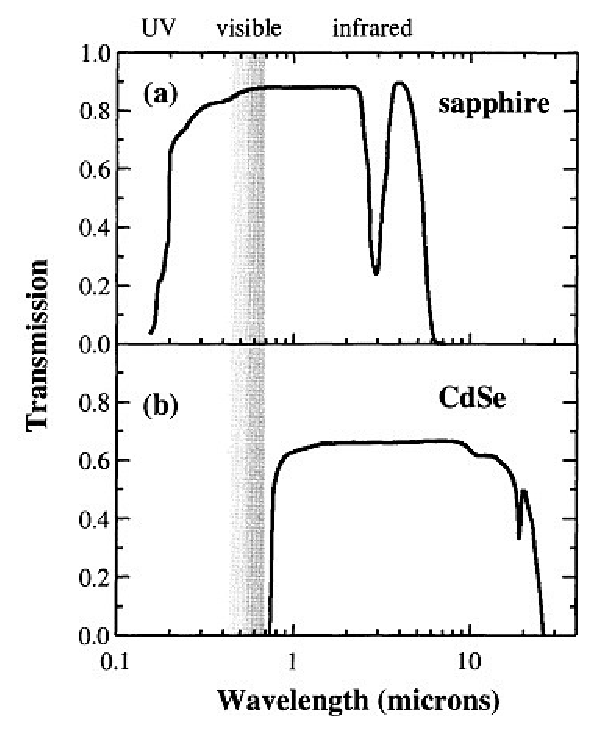
\includegraphics[width=60mm]{14.eps}
%\caption{default}
\label{fig:1.4}
\end{center}
\end{figure}

\begin{enumerate}
\marginnote{Fig. \ref{fig:1.4} (a)Transmission spectrum of a sapphire ($\mathrm{Al_2O_3}$) crystal of thickness 3 mm. (b) Transmission spectrum of a CdSe crystal of thickness 1.67 mm.}
  \item Sapphire has a high transmission in the wavelength range $0.2-6\um$. This defines the \textbf{transparency range} of the crystal. The transparency region of sapphire includes the whole of the visible spectrum, which explains why it appears colourless and transparent to the human eye.\marginnote{ Sapphire gemstones tend to be blue. This is caused by the presence of chromium, titanium and iron impurities in the $\mathrm{Al_2O_3}$ crystal. Pure synthetic $\mathrm{Al_2O_3}$ crystals are colorless.}
  \item Within the transparency range the absorption coefficient is very small, and the refractive index may be taken to be real with no imaginary component. The value of the refractive index is approximately constant, and is equal to 1.77 in sapphire.
  \item The transmission coefficient in the transparency range is determined by the reflectivity of the surfaces through eqn \ref{equa:1.6}. The reflectivity in turn is determined by the refractive index through eqn \ref{equa:1.26}. For sapphire with $n = 1.77$, this gives $R = 0.077$. Hence we find $T = (1 - R)^2 = 0.85$.
  \item The dip in the transmission in the infrared around $3\um$, and the sharp drop in the transmission for $\lambda > 6\um$, is caused by vibrational absorption. This absorption mechanism is analogous to the infrared absorption due to vibrations in polar molecules. The vibrational excitations of a crystal lattice are called phonon modes, and so the vibrational absorption in a solid is usually called phonon absorption or lattice absorption. This absorption mechanism will be discussed in Chapter \ref{chap:10}. \marginnote{Sapphire actually transmits in the far infrared spectral region when the frequency is well below that of the optical phonons.}
  \item The transmission drops sharply in the ultraviolet spectral region for $\lambda<0.2\um$ due to absorption by bound electrons. The onset of the absorption is called the \textbf{fundamental absorption edge}. The wavelength of the fundamental edge is determined by the band gap of the insulator. The explanation of the absorption spectra due to bound electrons needs band theory, and will be discussed in Chapters \ref{chap:3} and \ref{chap:4}.
\end{enumerate}


Point (1) is perhaps the most obvious aspect of the optical properties of insulators: they all tend to be colourless and transparent in the visible spectral region. If they are coloured, this is most likely caused by the presence of impurities, as will be explained in Section 1.4.5 below. This transparency is slightly deceptive. The insulators do absorb very strongly in the ultraviolet and in the infrared, but this is hidden from the human eye. The transparent region between the infrared and ultraviolet absorption bands is particularly useful for making optical windows and lenses. The approximate transparency range and refractive index of a number of common crystalline insulators are listed in Table 1.1. \marginnote{The very high transparency of diamond in the infrared is noteworthy. This is caused by the
fact that diamond is a purely covalent crystal, which means that its optical phonons cannot
interact directly with light waves. This point will be discussed further in Chapter 10.}

The crystallinity of the materials gives rise to a number of properties relating to the underlying symmetry of the lattice. This point will be expanded further in Section 1.5.1. One immediate consequence is that some of the materials listed in Table 1.1 are birefringent. The optical properties are anisotropic, and the value of the refractive index depends on the direction of propagation of the light relative to the crystallographic axes. The phenomenon of birefringence will be described in more detail in Section 2.4.

\marginnote{ Tab. \ref{tab:1.1} Approximate transparency range and refractive index $n$ of a number of crystalline insulators. $n$ is measured at 546 nm. Values of $n$ are given both for the o-ray and e-ray of birefringent materials.
\begin{minipage}{\textwidth}
\begin{tabular}{lll}\label{tab:1.1}
Crystal & Transparency & n\\
* & range($\um$) &* \\
$\mathrm{Al_2O_3}$ & 0.2-6 & 1.771 (o)\\
(sapphire) & *& 1.763 (e)\\
$\mathrm{BaF_2}$& 0.2-12 &1.476\\
Diamond & 0.25-80 & 2.424\\
KBr & 0.3-30 & 1.564\\
KCl &0.21-25 & 1.493\\
KI & 0.3-40 & 1.673\\
$\mathrm{MgF_2}$ & 0.12-8 & 1.379 (o)\\
* & * & 1.390 (e)\\
NaCl & 0.21-20 & 1.55\\
NaF & 0.19-15 & 1.326\\
$\mathrm{SiO_2}$ & 0.2-3 & 1.546 (o)\\
(quartz) & * & 1.555 (e)\\
$TiO_2$ & 0.45-5 & 2.652 (o)\\
(rutile) &* & 2.958 (e)
\end{tabular}
\end{minipage}
}

The optical properties of semiconductors are conceptually similar to those of insulators, except that the electronic and vibrational transitions occur at longer wavelengths. By way of example, Fig. 1.4(b) shows the transmission spectrum of the II-VI compound semiconductor CdSe over the same wavelength range as for the sapphire crystal. Just as with sapphire, we have a transparency range which is limited by electronic absorption at short wavelengths and lattice absorption at long wavelengths. The maximum transmission is around $60\%$ which is again mainly limited by the surface reflectivities. The short wavelength edge occurs beyond 700 nm, which means that the whole of the transparency range lies outside the visible spectrum. Hence no visible light is transmitted through the crystal, and it has a dark metallic appearance to the eye.

Table 1.2 lists the transparency range and refractive index of several semiconductors. The data show that the lower limit of the transmission range coincides closely with the wavelength of the fundamental band gap. This happens because the band gap determines the lowest energy for interband transitions, as will be explained in Chapter \ref{chap:3}. Note that the refractive index increases as the band gap wavelength gets larger.
\marginnote{Approximate transparency range, band gap wavelength $\lambda_g$, and refractive index $n$ of a number of common semiconductors. $n$ is measured at $10\um$.
\begin{minipage}{0.8\textwidth}
\begin{tabular}{llll}\label{tab:1.2}
Crystal & Transparency & $\lambda_g$ & $n$\\
* & range($\um$) & ($\um$) & * \\
Ge & 1.8-23 & 1.8 & 4.00\\
Si & 1.2-15 & 1.1 & 3.42\\
GaAs & 1.0-20 & 0.87 & 3.16\\
CdTe & 0.9-14 & 0.83 & 2.67\\
CdSe & 0.75-24 & 0.71 & 2.50\\
ZnSe & 0.45-20 & 0.44 & 2.41\\
ZnS & 0.4-14 & 0.33 & 2.20\\
\end{tabular}
\end{minipage}}

The upper limit of the transmission range is determined by the lattice absorption, as for insulators, and also by free carrier absorption. Free carriers are present in semiconductors at room temperature through the thermal excitation of electrons across the band gap or due to the presence of impurities. This causes infrared absorption, as will be explained in Section 7.4. Insulators have very small free carrier densities due to their large band gaps.



One very important aspect of the optical properties of semiconductors is that a subset of them, namely those with direct band gaps, luminesce strongly when electrons are promoted to the conduction band. This is the physical basis for the light-emitting devices used in the optoelectronics industry. The physical processes behind the luminescence will be explained in Chapter 5. The main point is that the wavelength of the luminescence coincides with the band gap of the semiconductor. In Chapter \ref{chap:10} we will see how quantum size effects in low-dimensional semiconductors can be used to shift the effective band gap to higher energy. This is a highly desirable feature, because it provides a way to \lq tune \rq the emission wavelength by controlled variation of the parameters during the crystal growth.

\marginnote{Refractive index of synthetic fused silica versus wavelength.
\begin{minipage}{0.8\textwidth}
\begin{tabular}{ll}\label{tab:1.3}
Wavelength(nm) & Refractive index\\
213.9 & 1.53430\\
239.9 & 1.51336\\
275.3 & 1.49591\\
334.2 & 1.47977\\
404.7 & 1.46962\\
467.8 & 1.46429\\
508.6 & 1.46186\\
546.1 & 1.46008\\
632.8 & 1.45702\\
706.5 & 1.45515\\
780.0 & 1.45367\\
1060 & 1.11968\\
1395 & 1.44583\\
1530 & 1.44427\\
1970 & 1.43853\\
2325 & 1.43293\\
\end{tabular}
\end{minipage}
}

\subsection{Glasses}

Glasses are extremely important optical materials. They have been used for centuries in prisms and lenses for optical instruments, in addition to their common usage in windows and glassware. In more recent times they have found new applications in optical fibre technology. With the exception of stained glasses, they are usually made to be transparent in the visible spectrum. They are not crystalline solids, and therefore do not exhibit the optical anisotropy that is characteristic of some crystals.

Most types of glasses are made by fusing sand (silica: $\mathrm{SiO_2}$) with other chemicals. Pure fused silica is an insulator, and shows all the characteristic features of insulators discussed in the previous section. It is transparent in the visible region, but absorbs in the ultraviolet due to the electronic transitions of the $\mathrm{SiO_2}$ molecules, and in the infrared due to vibrational absorption. The transparency range thus goes from around 200 nm in the ultraviolet to beyond 2000 nm in the infrared.

The properties of fused silica will be described in more detail in Section 2.2.3. Fused silica is used extensively in the fibre optics industry, as the principal material from which many fibres are made. It has been refined to such an extent that the absorption and scattering losses are so small that light can travel many kilometres down the fibre before being fully attenuated.

The refractive index of silica in the transparency range is tabulated against the wavelength in Table 1.3. This variation of the refractive index with wavelength is called dispersion. Note that it is not a very large effect: $n$ changes by less than $1\%$ over the whole visible spectral region. Note also that the dispersion is largest at the shortest wavelengths near the fundamental absorption edge. Dispersion is present in all optical materials, as will be explained in Section 2.3.

\begin{table}[htbp]\footnotesize
%\caption{Composition, refractive index and ultraviolet transmission of common glasses. The letters after the names give the abbreviations used to identify the glass type. The composition figures are the percentage by mass. The refractive index is measured at 546.1 nm, and the transmission is for a 1 cm plate at 310 nm.}
\begin{tabular}{cccccccccccc}

Name & $\mathrm{SiO_2}$&$\mathrm{B_2O_3}$&$\mathrm{Al_2O_3}$&$\mathrm{Na_2O}$&$\mathrm{K_2O}$&$\mathrm{CaO}$&$\mathrm{PbO}$&$n$&$T$\\

Fused silica &100&&&&&&&1.460 &0.91\\
Crown(K)&74&&&9&11&6&&1,513&0.4\\
BK&70&10&&8&8&1&&1.519&0.35\\
PK&&3&10&&12&5&&1.527&0.46\\
LF&53&&&5&8&&34&1.585&0.008\\
F&47&&&2&7&&44&1.607&\\
SF&33&&&&5&&62&1.746&\\

\end{tabular}
\label{tab:1.1}
\end{table}%

Chemicals are commonly added to silica during the fusion process to produce a whole range of other types of glasses. The presence of these additives can alter the refractive index and the transmission range. Table 1.4.2 lists the composition of a number of common glasses together with their refractive index and ultraviolet transmission. It is apparent that the additives have the effect of increasing the refractive index, at the expense of increasing the ultraviolet absorption. A high refractive index is desirable for cut-glass products, since it increases the reflectivity (see Exercise 1.2), and hence gives the glassware a more shiny appearance.

Stained glass and colour glass filters are made by adding semiconductors with band gaps in the visible spectral region during the fusion process. The properties of these coloured glasses will be discussed further in Section 1.4.5 below.

\begin{figure}
  \centering
  % Requires \usepackage{graphicx}
  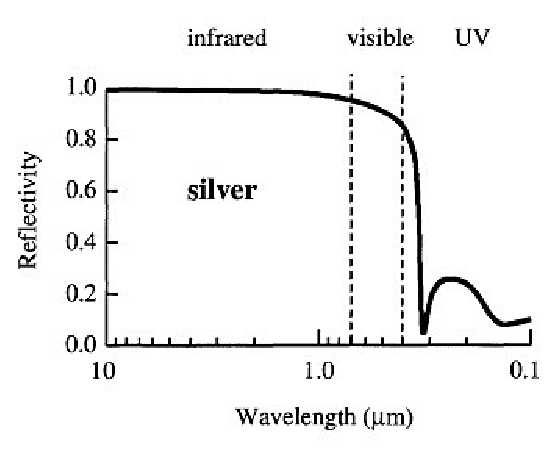
\includegraphics[width=0.4\textwidth]{15.eps}\label{fig:1.5}\\
\end{figure}\marginnote{Reflectivity of silver from the infrared to the ultraviolet.}

\subsection{Metals}

The characteristic optical feature of metals is that they are shiny. This is why metals like silver and aluminum have been used for making mirrors for centuries. The shiny appearance is a consequence of their very high reflection coefficients. We will see in Chapter 7 that the high reflectivity is caused by the interaction of the light with the free electrons that are present in the metal.

Figure 1.5 shows the reflectivity of silver from the infrared spectral region to the ultraviolet. We see that the reflectivity is very close to $100 \%$ in the infrared, and stays above $80 \%$ throughout the whole visible spectral region. The reflectivity then drops sharply in the ultraviolet. This general behaviour is observed in all metals. There is strong reflection for all frequencies below a characteristic cut-off frequency called the plasma frequency. The plasma frequency corresponds to a wavelength in the ultraviolet spectral region, and so metals reflect infrared and visible wavelengths, but transmit ultraviolet wavelengths. This effect is called the ultraviolet transmission of metals.

Some metals have characteristic colours. Copper, for example, has a pinkish colour, while gold is yellowish. These colours are caused by interband electronic transitions that occur in addition to the free carrier effects that cause the reflection. This point will be explained in Section 7.3.2 of Chapter \ref{chap:7}.

\subsection{Molecular materials}

The term `molecular material' could in principle cover the solid phase of any molecule. However, the crystalline phase of inorganic molecules such as NaCl or GaAs are classified as insulators or semiconductors in this book, while simple organic molecules such as methane ($\mathrm{CH_4}$) tend to be gases or liquids at room temperature. We therefore restrict our attention here to large organic molecules.

Some organic compounds form crystals in the condensed phase, but many others are amorphous. The solids are held together by the relatively weak van der Waals interactions between the molecules, which are themselves held together by strong covalent bonds. The optical properties of the solid therefore tend to be very similar to those of the individual molecules.

Organic compounds can be generally classified into either saturated or conjugated systems. This classification depends on the type of bonding in the molecule, and will be explained in more detail in Chapter \ref{chap:8}.

In saturated compounds, the valence electrons are incorporated into strong, localized bonds between neighbouring atoms. This means that all the electrons are tightly held in their bonds, and can only respond at high frequencies in the ultraviolet spectral range. Saturated compounds are therefore usually colourless and do not absorb in the visible region. Their properties are generally similar to those of the glasses discussed in Section 1.4.2 above: they absorb in the infrared and ultraviolet due to vibrational and electronic transitions respectively, and are transparent in the visible. Plastics such as poly-methyl-methacrylate (commonly known as `perspex' or `plexiglass') or poly-ethylene (polythene) are typical examples.

Conjugated molecules, by contrast, have much more interesting optical properties. The electrons from the $p$-like atomic states of the carbon atoms form large delocalized orbitals called $\pi$ orbitals which spread out across the whole molecule. The standard example of a conjugated molecule is benzene ($\mathrm{C_6H_6}$), in which the $\pi$ electrons form a ring-like orbital above and below the plane of the carbon and hydrogen atoms. Further examples include the other aromatic hydrocarbons, dye molecules, and conjugated polymers.

$\pi$ electrons are less tightly bound than the electrons in saturated molecules, and are optically-active at lower frequencies. In benzene the absorption edge is in the ultraviolet at 260 nm, but with other molecules the transition energy is shifted down to visible frequencies. The molecules with visible absorption also tend to emit strongly at visible frequencies. This makes them of high technological interest for applications as light-emitting devices. These are the solid state counterparts of the organic dyes that have been used in liquid lasers for several decades.

The optical processes that occur in $\pi$ conjugated materials will be described in Chapter \ref{chap:8}. By way of example, Fig. 1.6 shows the absorption spectrum of the technologically important polyftuorene-based polymer called `F8'. Thin film samples of this material are typically prepared by spin coating the molecules onto a glass slide. The data in Fig. 1.6 show that the polymer is transparent throughout most of the visible spectral region, but absorbs strongly at ultraviolet wavelengths. The broad absorption band which peaks at 380 nm is caused by vibrational-electronic transitions to the first singlet excited state of the molecule. This band extends slightly into the blue spectral region, and gives the material a pale yellow colour.

Conjugated polymers such as F8 luminesce strongly when electrons are promoted into the excited states of the molecule. The luminescence is Stokes shifted to lower energy compared to the absorption, and typically occurs in the middle of the visible spectral region. An attractive feature of these organic materials is that the emission wavelength can be 'tuned' by small alterations to the chemical structure of the molecular units within the polymers. We will see in Section 8.6 how this property has been used to develop organic light-emitting devices to cover the full range of the visible spectral region.

\begin{figure}[htbp]
  \centering
  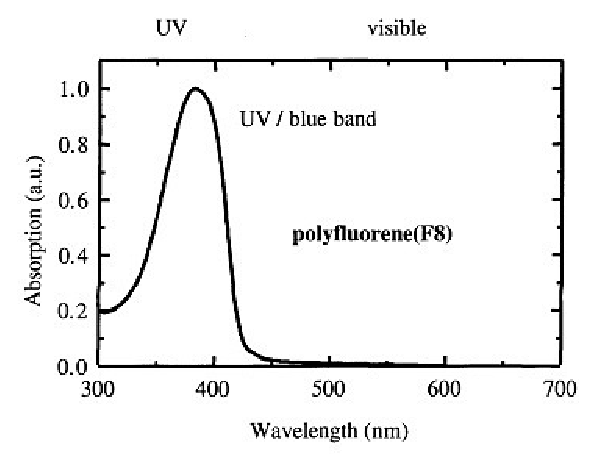
\includegraphics[width=0.4\textwidth]{16.eps}\\ \label{fig:1.6}
\end{figure}\marginnote{Absorption spectrum of the polyftuorene-based polymer F8 [poly(9,9-dioctylftuorene)]. After [5], \copyright 2001 Exerpta Medica Inc., reprinted with permission.}

\subsection{Doped glasses and insulators}

We have already mentioned in Section 1.4.2 above that colour glass filters and stained glass are made by adding appropriately chosen semiconductors to silica during the fusion process. This is a typical example of how a colourless material such as fused silica can take on new properties by controlled doping with optically active substances.

The colour of a colour glass filter can be controlled in two different ways.
\begin{enumerate}
  \item The most obvious way is by variation of the composition of the dopant. For example, the glass might be doped with the alloy semiconductor $\mathrm{Cd_xZn_{1-x}Se}$ during the fusion process, with the value of $x$ determined by the ZnSe $:$ CdSe ratio in the original melt. The band gap of the alloy can be `tuned' through the visible spectrum region by varying $x$, and this determines the short wavelength transmission cut-off for the filter.
  \item The size of the semiconductor crystallites within the glass can be very small, and this can also have an effect on the colour produced. Normally, the optical properties of a material are independent of the size of the crystal, but this ceases to be the case if the dimensions are comparable to the electron wavelength. The `quantum size effect' increases the energy of the electrons and hence shifts the effective band gap to higher energy. This point will be explained further in Section 6.9 of Chapter \ref{chap:6}.
\end{enumerate}

\begin{figure}
  \centering
  % Requires \usepackage{graphicx}
  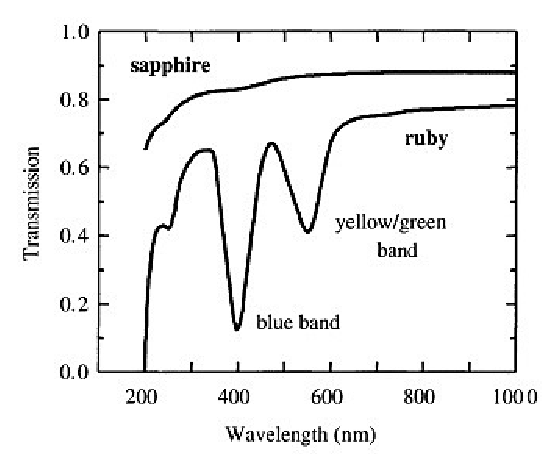
\includegraphics[width=0.4\textwidth]{17.eps}\\
  \label{fig:1.7}
\end{figure}\marginnote{
Transmission spectrum of ruby ($\mathrm{Al_2O_3}$ with $\mathrm{0.05\%Cr^{3+}}$) compared to sapphire (pure $\mathrm{Al_2O_3}$). The thicknesses of the two crystals were 6.1 mm and 3.0 mm respectively. After [6], reprinted with permission.
}


The principle of doping optically active atoms into colourless hosts is employed extensively in the crystals used for solid state lasers. A typical example is the ruby crystal. Rubies consist of $\mathrm{Cr^{3+}}$ ions doped into $\mathrm{Al_2O_3}$ (sapphire). In the natural crystals, the $\mathrm{Cr^{3+}}$ ions are present as impurities, but in synthetic crystals, the dopants are deliberately introduced in controlled quantities during the crystal growth process.

Figure 1.7 compares the transmission spectra of synthetic ruby ($\mathrm{Al_2O_3}$ with $0.05 \% \mathrm{Cr^{3+}}$) to that of synthetic sapphire (pure $\mathrm{Al_2O_3}$). It is seen that the presence of the chromium ions produces two strong absorption bands, one in the blue spectral region and the other in the green/yellow region. These two absorption bands give rubies their characteristic red colour. The other obvious difference between the two transmission curves is that the overall transmission of the ruby is lower. This is caused in part by the increased scattering of light by the impurities in the crystal.

The optical properties of crystals like ruby will be covered in Chapter \ref{chap:9}. We will see there that the broadening of the discrete transition lines of the isolated dopant ions into absorption bands is caused by vibronic coupling between the valence electrons of the dopant and the phonons in the host crystal. We will also see how the centre wavelength of the bands is determined by the crystal field effect, that is, the interaction between the dopant ions and electric field of the host crystal. These properties are very important in the design of solid state lasers and phosphors.

\section{Characteristic Optical Physics in the Solid State}

The previous section has given a brief overview of the optical properties of several different classes of solid state materials. It is natural to ask whether any of these properties are exclusive to the solid state. In other words, how do the optical properties of a solid differ from those of its constituent atoms or molecules? This question is essentially the same as asking what the difference is between solid state and atomic or molecular physics.

The answer clearly depends on the type of material that we are considering. In some materials there will be a whole range of new effects associated with the solid state, while with others, the differences may not be so great. Molecular materials are an example of the second type. We would expect the absorption spectra of a solid film and that of an equivalent dilute solution to be very similar. This happens because the forces between the molecules in the condensed phase are relatively weak compared to the forces within the molecule itself. The appeal of the solid state in this case is the high number density of molecules that are present, and the possibility of incorporating them into solid state electronic devices.

With many other materials, however, there will be substantial differences between the condensed phase and the gaseous or liquid state. It is obviously not possible to give a full catalogue of these effects in an introductory chapter such as this one. Instead, we will highlight here five aspects that make the physics of the solid state interesting and different, namely
\begin{itemize}
  \item Crystal symmetry
  \item Electronic bands
  \item Vibronic bands
  \item The density of states
  \item Delocalized states and collective excitations.
\end{itemize}
There are many others, of course, but these themes occur over and over again and are therefore worth considering briefly in themselves before we start going into the details.

\subsection{Crystal symmetry}

Most of the materials that we will be studying occur as crystals. Crystals have long range \textbf{translational order}, and can be categorized into 32 classes according to their \textbf{point group symmetry}. The point group symmetry refers to the group of symmetry operations that leaves the crystal invariant. Examples of these include rotations about particular axes, reflections about planes, and inversion about points in the unit cell. Some crystal classes such as the cubic ones possess a very high degree of symmetry. Others have much lower symmetry.

The link between the measurable properties and the point group symmetry of a crystal can be made through \textbf{Neumann's principle}. This states that:
\begin{quote}
  Any macroscopic physical property must have at least the symmetry of the crystal structure.
\end{quote}
For example, if a crystal has four-fold rotational symmetry about a particular axis, then we must get the same result in any experiment we might perform in the four equivalent orientations.
\begin{figure}[htbp]
  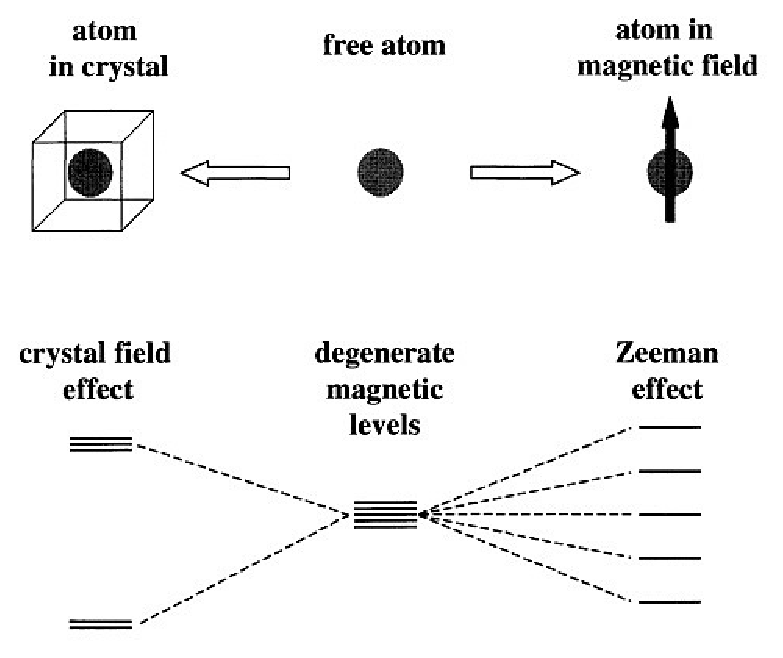
\includegraphics[width=0.6\textwidth]{18.eps}\\
  \label{fig:1.8}
\end{figure}
\marginnote{Splitting of the magnetic levels of a free atom by the crystal field effect. In the free atoms, the magnetic levels are degenerate. We must apply a magnetic field to split them by the Zeeman effect. However, the magnetic levels can be split even without applying an external magnetic field in a crystal. The details of the way the levels split are determined by the symmetry class of the crystal.}


It is instructive to compare the properties of a crystal to those of the atoms from which it has been formed. A gas of atoms has no translational order. Therefore we expect to find new effects in the solid state that reflect its translational symmetry. The formation of electronic bands and delocalized states discussed in Sections 1.5.2 and 1.5.5 below are examples of this. At the same time, the point group symmetry of a crystal is lower than that of the individual atoms, which have the highest possible symmetry due to their spherical invariance. We therefore expect to find other effects in the solid state that relate to the lowering of the symmetry on going from free atoms to the particular point group of the crystal class. Two specific examples of this are discussed briefly here, namely \textbf{optical anisotropy} and the \textbf{lifting of degeneracies}.

A crystal is said to be anisotropic if its properties are not the same in all directions. Anisotropy is only found in the solid state, because gases and liquids do not have any preferred directions. The degree of anisotropy found in a crystal depends strongly on the point group symmetry that it possesses. In cubic crystals, for example, the optical properties must be the same along the $x$, $y$ and $z$ axes because they are physically indistinguishable. On the other hand, in a uniaxial crystal, the properties along the optic axis will be different from those along the axes at right angles to it. The optical anisotropy is manifested by the property of birefringence which is discussed in Section 2.4. It is also important for the description of the nonlinear optical coefficients of crystals discussed in Chapter \ref{chap:11}.

The lifting of degeneracies by reduction of the symmetry is a well-known effect in atomic physics. Free atoms· are spherically symmetric and have no preferred directions. The symmetry can be broken by applying an external magnetic or electric field which creates a preferred axis along the field direction. This can lead to the lifting of certain level degeneracies that are present in the free atoms. The Zeeman effect, for example, describes the splitting of degenerate magnetic levels when a magnetic field is applied. If the same atom is introduced into a crystal, it will find itself in an environment with a point group symmetry determined by the lattice. This symmetry is lower than that of the free atom, and therefore some level degeneracies can be lifted.

This point is illustrated schematically in Fig. 1.8, which shows how the magnetic levels of a free atom can be split by the crystal field effect in an analogous way to the Zeeman effect. The splitting is caused by the interaction of the orbitals of the atoms with the electric fields of the crystalline environment. The details do not concern us here. The important point is that the splittings are determined by the symmetry class of the crystal and do not require an external field. Optical transitions between these crystal-field split levels often occur in the visible spectral region, and cause the material to have very interesting properties that are not found in the free atoms. These effects will be explored in more detail in Chapter \ref{chap:9}.

Before closing this section on crystal symmetry, it is worth pointing out that many important solid state materials do not possess long range translational symmetry. Glass is an obvious example. Other examples include thin molecular films such as light-emitting polymers sputtered onto substrates, and amorphous silicon. \marginnote{
\begin{minipage}{\textwidth}
    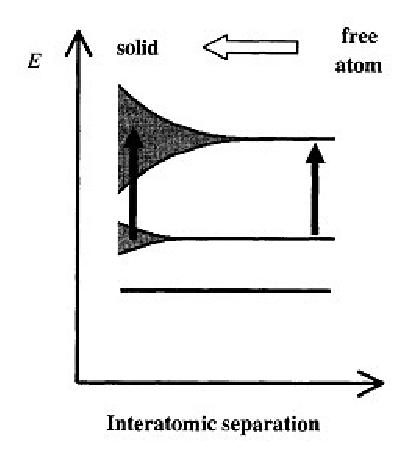
\includegraphics[width=25mm]{19.eps}
    \label{fig:1.9}
  \end{minipage}
 \\ [\intextsep]
Schematic diagram of the formation of electronic bands in a solid from the condensation of free atoms. As the atoms are brought closer together to form the solid, their outer orbitals begin to overlap with each other. These overlapping orbitals interact strongly, and broad bands are formed. The inner core orbitals do not overlap and so remain discrete even in the solid state. Optical transitions between the bands can occur, and this causes strong absorption over a continuous range of frequencies rather than discrete lines.}
The optical properties of these materials may be very similar to those of their constituent atoms or molecules. Their importance is usually related to the convenience of the solid phase rather than to new optical properties that relate to the solid state physics.

\subsection{Electronic bands}



The atoms in a solid are packed very close to each other, with the interatomic separation approximately equal to the size of the atoms. Hence the outer orbitals of the atoms overlap and interact strongly with each other. This broadens the discrete levels of the free atoms into bands, as illustrated schematically in Fig. 1.9.

The electron states within the bands are delocalized and possess the translational invariance of the crystal. \textbf{Bloch's theorem states} that the wave functions should be written in the form:
\begin{equation}\label{equa:1.27}
  \psi_{\mathrm{k}}(\mathrm{r})=u_{\mathrm{k}(\mathrm{r})}\exp(i\mathrm{k}\cdot \mathrm{r})
\end{equation}
where $u_k(r)$ is a function that has the periodicity of the lattice. The Bloch states described by eqn \ref{equa:1.27} are modulated plane waves. Each electronic band has a different envelope function $u_k (r)$ which retains some of the atomic character of the states from which the band was derived.

Optical transitions can occur between the electronic bands if they are allowed by the selection rules. This \lq interband\rq absorption is possible over a continuous range of photon energies determined by the lower and upper energy limits of the bands. This contrasts with the absorption spectra of free atoms, which consist of discrete lines. The observation of broad bands of absorption rather than discrete lines is one of the characteristic features of the solid state.

Interband transitions will be discussed at length in a number of chapters in this book, most notably Chapters \ref{chap:3} and \ref{chap:5}. The absorption strength is usually very high because of the very large density of absorbing atoms in the solid. This means that we can produce sizeable optical effects in very thin samples, allowing us to make the compact optical devices that form the basis of the modem optoelectronics industry.

\subsection{Vibronic bands}

The electronic states of the atoms or molecules in a solid may be strongly coupled to the vibrational modes of the crystal through the vibronic interaction. A typical example of where this effect occurs is the doped insulator crystals introduced in Section 1.4.5. The vibronic coupling broadens the discrete electronic states of the isolated dopant atoms into bands. This has the effect of broadening the discrete absorption and emission lines of the atoms into continuous bands. These vibronic effects will be described in more detail in Chapter \ref{chap:9}.

It is important to realize that the reason for the formation of the vibronic bands is different to that for the electronic bands considered in the previous section. In the case of vibronic bands, the continuum of states arises from the coupling of discrete electronic states to a continuous spectrum of vibrational modes. This contrasts with the electronic bands, where the continuum arises from interactions between electronic states of neighbouring atoms.

Vibronic effects are also observed in molecular materials. This is an interesting case which highlights the difference between the solid state and the liquid or gaseous phase. The absorption spectra of simple free molecules also show vibrational-electronic bands, but the transition frequencies are discrete because both the electronic energies and the vibrational energies are discrete.  In molecular solids, by contrast, the vibrational frequencies are continuous, and this causes continuous absorption and emission spectra.

\subsection{The density of states}

The concept of the \textbf{density of states} is an inevitable corollary of band formation in solids. The electronic and vibrational states of free molecules and atoms have discrete energies, but this is not the case in a solid: both the electronic states and the phonon modes have a continuous range of energies. This continuum of states leads to continuous absorption and emission bands, as has already been stressed in the previous two sections.

The number of states within a given energy range of a band is conveniently expressed in terms of the density of states function $g(E)$. This is defined as:
\begin{equation}\label{equa:1.28}
    \text{\footnotesize{Number of states in the range}}\quad E\rightarrow(E+dE)=g(E)dE
\end{equation}
$g(E)$ is worked out in practice by first calculating the density of states in momentum space $g(k)$, and then using the relationship between $g(E)$ and $g(k)$, namely:
\begin{equation}\label{equa:1.29}
  g(E)=g(k)\frac{dk}{dE}
\end{equation}
This can be evaluated from know ledge of the $E-k$ relationship for the electrons or phonons. Knowledge of $g(E)$ is crucial for calculating the absorption and emission spectra due to interband transitions and also for calculating the shape of vibronic bands.

\subsection{Delocalized states and collective excitations}

The fact that the atoms in a solid are very close together means that it is possible for the electron states to spread over many atoms. The wave functions of these delocalized states possess the underlying translational symmetry of the crystal. The Bloch waves described by eqn \ref{equa:1.27} are a typical example. The delocalized electron waves move freely throughout the whole crystal and interact with each other in a way that is not possible in atoms. The delocalization also allows collective excitations of the whole crystal rather than individual atoms. Two examples that we will consider in this book are the excitons formed from delocalized electrons and holes in a semiconductor, and the plasmons formed from free electrons in metals and doped semiconductors. These collective excitations may be observed in optical spectra, and have no obvious counterpart in the spectra of free atoms. These excitonic effects will be discussed in Chapter \ref{chap:4}, while plasmons are covered in Section 7.5.

Other wave-like excitations of the crystal are delocalized in the same way as the electrons. In the case of the lattice vibrations, the delocalized excitations are described by the phonon modes. We have already mentioned above that the phonon frequencies are continuous, which contrasts with the discrete vibrational frequencies of molecules. Some optical effects related to phonons have direct analogies with the vibrational phenomena observed in isolated molecules but others are peculiar to the solid state. Examples of the former are Raman scattering and infrared absorption. Examples of the latter include the phonon-assisted interband transitions in semiconductors with indirect band gaps (cf. Section 3.4), and the broadening of the discrete levels of impurity atoms into continuous vibronic bands by interactions with phonons as discussed in Chapter \ref{chap:9}.

The delocalized states of a crystal are described by quantum numbers such as $\mathrm{k}$ and $\mathrm{q}$ which have the dimensions of inverse length. These quantum numbers follow from the translational invariance, and are therefore a fundamental manifestation of the crystal symmetry. To all intents and purposes, the quantum numbers like $\mathrm{k}$ and $\mathrm{q}$ behave like the wave vectors of the excitations, and they will be treated as such whenever we encounter them in derivations. However, it should be borne in mind that this is really a consequence of the deep underlying symmetry which is unique to the solid state.

\section{Microscopic Models}

In the following chapters we will be developing many microscopic models to explain the optical phenomena that are observed in the solid state. The types of models will obviously vary considerably, but they can all be classified into one of the following three general categories:
\begin{itemize}
  \item Classical
  \item Semiclassical
  \item Fully quantum
\end{itemize}
These approaches get progressively more difficult, and so we usually apply them in the order listed above.

In the classical approach we treat both the medium and the light according to classical physics. The dipole oscillator model described in Chapter \ref{chap:2} is a typical example. This model is the basic starting point for understanding the general optical properties of a medium, and in particular for describing the main effects due to free electrons (Chapter \ref{chap:7}) and phonons (Chapter \ref{chap:10}). We will also use it as a starting point for the discussion of nonlinear optics in Chapter \ref{chap:11}. It would be a mistake to undervalue the classical approach in this modem day and age. The value of more sophisticated models will only be appreciated fully once the classical physics has been properly understood.

In semiclassical models we apply quantum mechanics to the atoms, but treat the light as a classical electromagnetic wave. The treatment of interband absorption in Chapter \ref{chap:3} is a typical example. The absorption coefficient is calculated using Fermi's golden rule, which requires knowledge of the wave functions of the quantized levels of the atoms, but treats the light-matter interaction as that between a quantized atom and a classical electric field wave. This semiclassical approach is used extensively throughout the book. Appendix B summarizes the main results that will be needed.

The final approach is the full quantum treatment. This is the realm of quantum optics, where both the atoms and the light are treated quantum mechanically. We use this approach implicitly whenever we refer to the light as a beam of photons and draw Feynman diagrams to represent the interaction  processes that are occurring. This might give the impression that the explanations we are giving are fully quantum because we speak in terms of photons interacting with atoms. However, in the equations used to describe the process quantitatively, the light is treated classically and only the atoms are quantized. The quantitative description is therefore only semiclassical. The use of the fully quantum approach at the quantitative level is beyond the scope of this present book.

\section*{Chapter Summary}

\definecolor{shadecolor}{rgb}{1.0,0.9,0.9}
\begin{shaded}
\begin{itemize}
  \item The propagation of light through a medium is quantified by the complex refractive index $\tilde{n}$. The real part of $\tilde{n}$ determines the velocity of light in the medium, while the imaginary part determines the absorption coefficient. Beer's law (eqn. \ref{equa:1.4}) shows that the intensity of light in an absorbing medium decays exponentially.
  \item Reflection occurs at the interface between two optical materials with different refractive indices. The coefficient of reflectivity can be calculated from the complex refractive index using eqn \ref{equa:1.26}.
  \item The transmission of a sample is determined by the reflectivities of the surfaces and the absorption coefficient through eqn \ref{equa:1.6}.
  \item The complex refractive index is related to the complex dielectric constant through eqn \ref{equa:1.19}. The relationships between the real and imaginary parts of $\tilde{n}$ and $\tilde{\epsilon_r}$ are given in eqns \ref{equa:1.20}-\ref{equa:1.25}.
  \item Luminescent materials re-emit light by spontaneous emission after absorbing photons. The frequency shift between the emission and absorption is called the Stokes Shift.
  \item Scattering causes beam attenuation in accordance with Beer's law. The scattering is called elastic if the frequency is unchanged, and inelastic otherwise.
  \item The optical spectra of solid state materials usually consist of broad bands rather than sharp lines. The bands arise either from electronic interactions between neighbouring atoms or from vibronic coupling to phonon modes.
  \item Insulators and glasses have vibrational absorption at infrared wavelengths and electronic absorption in the ultraviolet spectral region. They are transparent and colourless in the visible spectral region between these two absorption bands. In semiconductors and molecular materials the electronic absorption occures at lower frequencies in the near infrared or visible spectral region.
  \item The free carriers present in metals make them highly reflective in the infrared and visible spectral regions. The colouration of some metals is caused by electronic interband absorption.
  \item The addition of optically active dopants to a colourless host crystal or glass produces the characteristic colours of stained glasses and gemstones.
  \item Crystals have both translational symmetry and point group symmetry. The consequences of the point group symmetry for the optical properties are determined by Neumann's Principle.
\end{itemize}
\end{shaded}

\section*{Further Reading}

A good general discussion of the optical properties of materials can be found in Hecht (1998). A more advanced treatment may be found in Born and Wolf (1999). The introduction to the optical properties of various materials given in Section 1.4 will be expanded in subsequent chapters, where suitable further reading will be suggested.

The relationship between the optical properties and the complex refractive index and dielectric constant is discussed in most texts on electromagnetism, for example, Bleaney and Bleaney (1976), or Lorrain, Corson and Lorrain (2000). This material is also covered in Born and Wolf (1999).

A classic discussion of the effects of the point group symmetry on the physical properties of crystals is given in Nye (1957).

\chapter{Classical Propagation}\label{chap:2}
\definecolor{shadecolor}{rgb}{0.9,0.9,0.9}
\begin{shaded}

The propagation of light through an optical medium was discussed in general terms in Sections 1.1-1.3 of Chapter \ref{chap:1}. We saw there that the propagation is characterized by two parameters, namely the refractive index and the absorption coefficient. In this chapter we will investigate the classical theory of optical propagation, in which the light is treated as electromagnetic waves and the atoms or molecules are modelled as classical dipole oscillators. We will see that this model gives a good general overview of the optical properties, and enables us to calculate the frequency dependence of the complex dielectric constant. This gives us the frequency dependence of the absorption coefficient and refractive index, and hence enables us to explain the phenomenon of dispersion. We will also see that the model provides the framework for describing the effects due to optical anisotropy such as birefringence.

The treatment given here presupposes a working knowledge of the electromagnetic properties of dielectrics. A summary of the main results that we will use is given in Appendix A. The model will be revisited in subsequent chapters when we consider the optical properties of free electrons in Chapter \ref{chap:7}, and when we discuss lattice vibrations in Chapter \ref{chap:10}. The model is also the starting point for the treatment of nonlinear optical effects in Chapter \ref{chap:11}.
\end{shaded}

\section{Propagation of Light in a Dense Optical Medium}

The classical model of light propagation was developed at the end of the nineteenth century following Maxwell's theory of electromagnetic waves and the introduction of the concept of the dipole oscillator. In this section we will give a qualitative discussion of the physical assumptions of this model, leaving the quantitative calculation to the next section.

The model assumes that there are several different types of oscillators within a medium, each with their own characteristic resonant frequency. At optical frequencies the most important contribution is from the oscillations of the \textbf{bound electrons} within the atoms, and so we begin this section by considering atomic oscillators. We then go on to introduce the idea of \textbf{vibrational oscillators}, which resonate at lower frequencies in the infrared spectral region, and finally mention \textbf{free electron oscillators}, which are responsible for the principal optical properties of metals.

\subsection{Atomic oscillators}
\marginnote{
\begin{minipage}{\textwidth}
    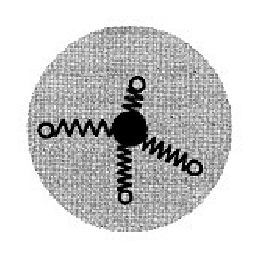
\includegraphics[width=25mm]{21.eps}
    \label{fig:2.1}
  \end{minipage}
 \\ [\intextsep]
Classical model of the bound electrons in an atom. The electrons are represented by the open circles, while the black circle at the centre of the atom represents the nucleus. The electrons are held to the heavy nucleus by springs which represent the restoring forces due to the binding between them. Each atom has a series of characteristic resonant frequencies which we now know to correspond with the quantized transition energies.}
The concept of the dipole oscillator was introduced soon after Maxwell's electromagnetic theory. It was shown theoretically that an oscillating electric dipole would emit electromagnetic waves, and this was confirmed in 1887 when Heinrich Hertz succeeded in generating and detecting radio waves in the laboratory. He used an oscillatory discharge across a spark gap as the source and a wire loop as the aerial of the detector. This was an elegant confirmation of the validity of Maxwell's electromagnetic theory, and the beginning of radio telecommunications.


The idea of considering atoms as oscillating dipoles was originally proposed by Henrick Antoon Lorentz in 1878, thus preceding Hertz's demonstration by several years. It was known that atoms emit and absorb at discrete frequencies, and Lorentz's model provided a simple explanation for these observations in terms of the newly discovered electromagnetic theories.

The oscillator model of the atom is illustrated schematically in Fig. 2.1. It is assumed that the electron is held in a stable orbit with respect to the nucleus, and the spring represents the restoring force for small displacements from the equilibrium. The negatively charged electron and the positively charged nucleus form an electric dipole with a magnitude proportional to their  separation. Lorentz, of course, could not have known about electrons and nuclei, because they were not discovered until 1897 and 1911 by J.J. Thomson and Ernest Rutherford respectively. Lorentz simply postulated the existence of dipoles without knowing their origin.

The natural resonant frequency $\omega_0$ of the atomic dipoles is determined by their mass and the magnitude of the restoring force experienced for small displacements. The appropriate mass is the \textbf{reduced mass} given by:
\begin{equation}\label{equa:2.1}
  \frac{1}{\mu}=\frac{1}{m_0}+\frac{1}{m_N}
\end{equation}
where $m_0$ and $m_N$ are the masses of the electron and nucleus respectively. Since $m_N\gg m_o$, we may safely take $\mu \approx m_o$ here. The restoring force is quantified in terms of a spring constant $K_s$, which is chosen so that $\omega_0$ coincides with one of the natural frequencies of the atoms (see Exercise 2.1):
\begin{equation}\label{equa:2.2}
  \omega_0=\sqrt{\frac{K_s}{\mu}}
\end{equation}
We have to suppose that there are several dipoles within every atom, to account for the fact that a given atom has many transition frequencies. These are known from the absorption and emission spectra, and the frequencies occur in the near-infrared, visible and ultraviolet spectral regions ($10^{14}-10^{15}$ Hz).

We can understand the connection between the atomic dipoles and the emission spectra by considering the oscillations of the dipole shown in Fig. 2.2. An electric dipole consists of a positive charge $+q$ at position $\mathrm{r}_{+}$ and a negative charge $-q$ at $r_{-}$. The electric dipole moment is defined as
\begin{equation}\label{equa:2.3}
  \mathrm{p}=q(\mathrm{r}_{+}-\mathrm{r}_{-})
\end{equation}
Hence the positive nucleus and negative electron form a dipole with magnitude equal to $e|\mathrm{r_N}-\mathrm{r}_e|$.

\begin{figure}[htbp]
  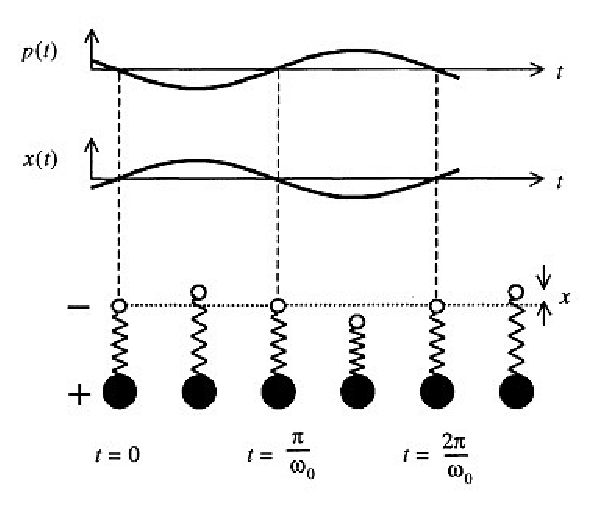
\includegraphics[width=0.6\textwidth]{22.eps}\\
  \label{fig:2.2}
\end{figure}\marginnote{Oscillations of a  classical dipole consisting of a heavy positive charge and a light negative charge bound together by a spring. $x(t)$ is the time-dependent displacement of the negative charge from its equilibrium position. The natural vibrations of the dipole about the equilibrium length at frequency $\omega_0$ generate a time dependent dipole moment $p(t)$ as indicated in the top half of the figure.}


During the oscillations of the atomic dipole, the nucleus remains more or less stationary due to its heavy mass, while the electron oscillates backwards and forwards at frequency $\omega_0$. Hence the oscillations produce a time varying dipole in addition to any permanent dipole the atom may have. The magnitude of the time varying dipole is given by:
\begin{equation}\label{equa:2.4}
p(t) = -ex(t),
\end{equation}
where $x(t)$ is the time varying displacement of the electron from its equilibrium position. This connection between the electron displacement and the time dependent atomic dipole is illustrated in the top half of Fig. 2.2. The oscillating dipole radiates electromagnetic waves at frequency $\omega_0$, in accordance with the theory of classical Hertzian dipoles. Hence the atom is expected to radiate light at its resonant frequency whenever sufficient energy is imparted to it to excite the oscillations.

\marginnote{We assume here that the forces exerted by the electric fields are very small compared to the binding forces that hold the electrons to the nucleus. This approximation may not be valid if we are using a very powerful laser beam to excite the medium. If this is the case, then we are working in the regime of nonlinear optics. These effects are considered in Chapter \ref{chap:11}.}

We can also use the dipole model to understand how the atom interacts with an external electromagnetic wave at frequency $\omega$. The AC electric field exerts forces on the electron and the nucleus and drives oscillations of the system at frequency $\omega$. If $\omega$ coincides with one of the natural frequencies of the atom, then we have a resonance phenomenon. This induces very large amplitude oscillations, and transfers energy from the external wave to the atom. The atom can therefore absorb energy from the light wave if $\omega=\omega_0$. The absorption strength is characterized by the absorption coefficient $\alpha$, and the intensity of the wave will decay exponentially according to Beer's law (eqn \ref{equa:1.4}).

We now know from quantum theory that what actually happens during absorption is that the atom jumps to an excited state by absorbing a photon. This can only occur if $\hbar\omega=E_2-E_1$, where $E_1$ and $E_2$ are the quantized energies of the initial and final states. Once it has been excited, the atom can return to the ground state by a series of radiationless transitions, in which case the energy from the absorbed photon is ultimately converted into heat. Alternatively, it can luminesce by re-emitting a photon at some later time. The re-radiated photons are incoherent with each other and are emitted in all directions rather than in the specific direction of the incoming wave. Hence there is a net decrease in the energy flow in the beam direction, which is equivalent to absorption.

If $\omega$ does not coincide with any of the resonant frequencies, then the atoms will not absorb, and the medium will be transparent. In this situation the light wave drives non-resonant oscillations of the atoms at its own frequency $\omega$. The oscillations of the atoms follow those of the driving wave, but with a phase lag. The phase lag is a standard feature of forced oscillators and is caused by damping. (See Exercise 2.2.) The oscillating atoms all re-radiate instantaneously, but the phase lag acquired in the process accumulates through the medium and retards the propagation of the wave front. This implies that the propagation velocity is smaller than in free space. The reduction of the velocity in the medium is characterized by the refractive index defined in eqn \ref{equa:1.2}.

The slowing of the wave due to the non-resonant interactions can be considered as a repeated scattering process. The scattering is both coherent and elastic, and each atom behaves like a Huygens point source. The scattered light interferes constructively in the forward direction, and destructively in all other directions, so that the direction of the beam is unchanged by the repetitive scattering process. However, each scattering event introduces a phase lag which causes a slowing of the propagation of the phase front through the medium.\marginnote{\begin{minipage}{\textwidth}
    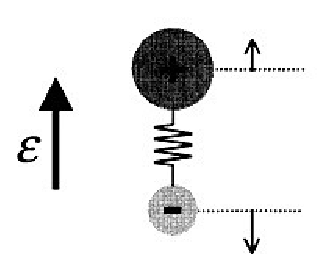
\includegraphics[width=25mm]{23.eps}
    \label{fig:2.3}
  \end{minipage}
 \\ [\intextsep]
Classical model of a polar molecule. The atoms are positively and negatively charged, and can vibrate about their equilibrium separation. These vibrations produce an oscillating electric dipole which will radiate electromagnetic waves at the resonant frequency. Alternatively, the molecule will interact with the electric field $\vec{\varepsilon}$ of a light wave through the forces exerted on the charged atoms.}

\subsection{Vibrational oscillators}

An optical medium may contain other types of dipole oscillators in addition to those originating from the bound electrons within the atoms. If the medium is ionic, it will contain oppositely charged ions. Vibrations of these charged atoms from their equilibrium positions within the crystal lattice will produce an oscillating dipole moment, in exactly the same way as the oscillations of the electrons within the individual atoms that we considered above. Therefore, we must also consider the optical effects dues to these vibrational oscillators when we consider the interaction of light with an ionic optical medium.

The optical effects of vibrational oscillators are well known in molecular physics. Figure 2.3 gives a schematic illustration of a classical polar molecule. This consists of two charged atoms bound together in a stable configuration, with the spring representing the molecular bond between them. The charged atoms can vibrate about their equilibrium positions and induce an oscillating electric dipole in an analogous way to the bound electrons in the atoms. We see immediately from eqn \ref{equa:2.2} that the vibrations will occur at lower frequencies because the reduced mass is larger. The vibrations therefore occur at infrared frequencies with $\omega/{2\pi}\sim 10^{12}-10^{13}$Hz. These molecular vibrations are associated with strong absorption lines in the infrared spectral region.

The interaction between the vibrations of the molecule and the light wave occurs through the forces exerted on the atoms by the electric field. It is obvious that this can only happen if the atoms are charged. This is why we specified that the molecule was \textbf{polar} in the preceding paragraph. A polar molecule is one in which the electron charge cloud that forms the bond sits closer to one of the atoms than to the other. Ionic molecules like the alkali halides (e.g. $\mathrm{Na^+C1^-}$) clearly fall into this category, while purely covalent ones such as the elemental molecules (e.g. $\mathrm{O_2}$) do not. Many other molecules fall somewhere between these two limits. Water ($\mathrm{H_2O}$) is a well known example. Oxygen has a greater electron affinity than hydrogen, and so the valence electrons in the $\mathrm{O-H}$ bond sit closer to the oxygen atoms. The two hydrogen atoms therefore possess a small positive charge which is balanced by a negative charge of twice the magnitude on the oxygen atom.

In a crystalline solid formed from the condensation of polar molecules, the atoms are arranged in an alternating sequence of positive and negative ions. The ions can vibrate about their equilibrium positions, and this produces oscillating dipole waves. These oscillations are associated with \textbf{lattice vibrations}, and they occur at frequencies in the infrared spectral region. We will consider the optical properties related to the lattice vibrations in detail in Chapter \ref{chap:10}. We will see there that the light-matter interaction is associated with the excitation of \textbf{phonons}, which are quantized lattice waves. At this stage, we simply note that the lattice vibrations of a polar crystal give rise to strong optical effects in the infrared spectral region. These effects occur in addition to those due to the bound electrons of the atoms that comprise the crystal. In practice we can treat these two types of dipoles separately because the resonances are sharp and they occur at very different frequencies. Therefore the resonant effects of the bound electrons are negligible at the frequencies of the lattice vibrations, and \textit{vice versa}. This point will be considered in more detail in Section 2.2.2.

\subsection{Free electron oscillators}
The electronic and vibrational dipoles considered above are both examples of bound oscillators. Metals and doped semiconductors, by contrast, contain significant numbers of \textbf{free electrons}. As the name implies, these are electrons that are not bound to any atoms, and therefore do not experience any restoring forces when they are displaced. This implies that the spring constant in eqn \ref{equa:2.2} is zero, and hence that the natural resonant frequency $\omega_0= 0$.

The free electron model of metals is attributed to Paul Drude, and so the application of the dipole oscillator model to free electron systems is generally called the \textbf{Drude-Lorentz model}. The dipole oscillator model is perfectly valid, except that we must set $\omega_0=0$ throughout. The optical properties of free electron systems will be discussed in Chapter \ref{chap:7}.

\section{The Dipole Oscillator Model}
In the previous section we introduced the general assumptions of the dipole oscillator model. We now want to use the model to calculate the frequency dependence of the refractive index and absorption coefficient. This will provide a simple explanation for the dispersion of the refractive index in optical materials, and will also illustrate a very general point that the phenomena of absorption and refraction are related to each other.

\subsection{The Lorentz oscillator}
We consider the interaction between a light wave and an atom with a single resonant frequency $\omega_0$ due to the bound electrons, as given by eqn \ref{equa:2.2}. We model the displacement of the atomic dipoles as damped harmonic oscillators. The inclusion of damping is a consequence of the fact that the oscillating dipoles can lose their energy by collisional processes. In solids, this would typically occur through an interaction with a phonon which has been thermally excited in the crystal. As we will see, the damping term has the effect of reducing the peak absorption coefficient and broadening the absorption line.

\marginnote{We know from experimental observations that atoms must have many natural resonant frequencies to account for the multiplicity of lines in the absorption and emission spectra. However, the salient features of the physical behaviour are well illustrated by a singly resonant system, and the inclusion of multiple resonances complicates the discussion without adding much to the physical understanding at this stage. We therefore postpone the discussion of the effects of multiple resonances to subsection 2.2.2 below.}

The electric field of the light wave induces forced oscillations of the atomic dipole through the driving forces exerted on the electrons. We make the assumption that $m_N\gg m_0$ here so that we can ignore the motion of the nucleus. The displacement $x$ of the electron is governed by an equation of motion of the form:
\begin{equation}\label{equa:2.5}
  m_0\frac{d^2x}{dt^2}+m_0\gamma\frac{dx}{dt}+m_0\omega_0^2x=-e\varepsilon,
\end{equation}
where $\gamma$ is the damping rate, $e$ is the magnitude of the electric charge of the electron, and $\varepsilon$ is the electric field of the light wave. The terms on the left hand side represent the acceleration, the damping and the restoring force respectively. The damping is modeled by a frictional force which is proportional to the velocity and impedes the motion. The term on the right hand side represents the driving force due to the AC electric field of the light wave.

We consider the interaction of the atom with a monochromatic light wave of angular frequency $\omega$. The time dependence of the electric field is given by
\begin{equation}\label{equa:2.6}
  \varepsilon(t)=\varepsilon_0\cos(\omega t+\Phi)=\varepsilon_0\mathfrak{Re}(\exp(-i\omega t-\Phi))
\end{equation}
where $\varepsilon_0$ is the amplitude and $\Phi$ is the phase of the light. In order to keep consistency with the sign convention introduced later, we have chosen to take the negative frequency part of the complex exponential.
\marginnote{Note that the phase factors $\Phi$ and $\Phi'$ in eqns \ref{equa:2.6} and \ref{equa:2.7} are not necessarily the same. In fact, the phase of the electrons will tend to lag behind the phase of the light. This is a well known property of forced oscillations: the vibrations occur at the same frequency as the driving force but lag behind due to the damping term. This phase lag is the origin of the slowing down of the light in the optical medium, as discussed above in Section 2.1.}

The AC electric field will drive oscillations at its own frequency $\omega$. We therefore substitute eqn \ref{equa:2.6} into eqn \ref{equa:2.5} and look for solutions of the form:
\begin{equation}\label{equa:2.7}
  x(t)=X_0\mathfrak{Re}(\exp(-i\omega t-\Phi')),
\end{equation}
where $X_0$ and $\Phi'$ are the amplitude and phase of the oscillations. We can incorporate the phase factors of eqns \ref{equa:2.6} and \ref{equa:2.7} into the amplitudes by allowing both $\varepsilon_0$ and $X_0$ to be complex numbers. We then substitute $\varepsilon(t)=\varepsilon_0e^{-i\omega t}$ into eqn \ref{equa:2.5}, and look for solutions of the form $x(t)=X_0e^{-i\omega t}$. This gives:
\begin{equation}\label{equa:2.8}
  -m_0\omega^2X_0e^{-i\omega t}-im_0\gamma\omega X_0e^{-i\omega t}+m_0\omega_0^2X_0e^{-i\omega t}=-e\varepsilon_0e^{-i\omega t}
\end{equation}
which implies that:
\begin{equation}\label{equa:2.9}
  X_0=\frac{-e\varepsilon_0/m_0}{\omega_0^2-\omega^2-i\gamma\omega}.
\end{equation}
The displacement of the electrons from their equilibrium position produces a time varying dipole moment $p(t)$, as shown in Fig. 2.2. The magnitude of the dipole is given by eqn 2.4. This gives a resonant contribution to the macroscopic polarization (dipole moment per unit volume) of the medium. If $N$ is the number of atoms per unit volume, the resonant polarization is given by:
\begin{eqnarray}\label{equa:2.10}
% \nonumber to remove numbering (before each equation)
\nonumber  P_{resonant} &=& Np \\
\nonumber   &=& -Nex \\
   &=& \frac{Ne^2}{m_0}\frac{1}{(\omega_0^2-\omega^2-i\gamma\omega)}\varepsilon
\end{eqnarray}
A quick inspection of eqn 2.10 shows that the magnitude of $P_{resonant}$ is small unless the frequency is close to $\omega_0$. This is another general property of forced oscillations: the response is small unless the frequency is close to resonance with the natural frequency of the oscillator.

Equation \ref{equa:2.10} can be used to obtain the complex relative dielectric constant $\epsilon_r$. The electric displacement $\mathrm{D}$ of the medium is related to the electric field $\vec{\varepsilon}$ and polarization $\mathrm{P}$ through:
\begin{equation}\label{equa:2.11}
  \mathrm{D}=\epsilon_0\vec{\varepsilon}+\mathrm{P}
\end{equation}
where the bold font indicates vector quantities (see eqn A.2 in Appendix A). We are interested in the optical response at frequencies close to $\omega_0$, and so we split the polarization into a non-resonant background term and the resonant term arising from the driven response of the oscillator. We therefore  write:\marginnote{The electric susceptibility $\chi$ in eqn \ref{equa:2.12} accounts for all other contributions to the polarizability of the atoms. We will discuss the physical meaning of the `non-resonant polarization' in subsection 2.2.2 below.}
\begin{eqnarray}\label{equa:2.12}
% \nonumber to remove numbering (before each equation)
\nonumber  \mathrm{D} &=& \epsilon_0\vec{\varepsilon}+\mathrm{P}_{background}+\mathrm{P}_{resonant} \\
  &=& \epsilon_0\vec{\varepsilon}+\epsilon_0\chi\vec{\varepsilon}+\mathrm{P}_{resonant}
\end{eqnarray}
To simplify the mathematics, we will assume that the material is isotropic, in which case the relative dielectric constant is defined through the relationship:
\begin{equation}\label{equa:2.13}
  \mathrm{D}=\epsilon_0\epsilon_r\mathrm{P}_{resonant}
\end{equation}
We then combine eqns \ref{equa:2.10}-\ref{equa:2.13} to obtain:\marginnote{The treatment of non-isotropic materials only introduces unnecessary complications at this stage, and will be covered briefly in Section 2.4.}
\begin{equation}\label{equa:2.14}
  \epsilon_r=1+\chi+\frac{Ne^2}{\epsilon_0m_0}\frac{1}{(\omega_0^2-\omega^2-i\gamma\omega)}.
\end{equation}
This can be spilt into its real and imaginary parts according to eqn \ref{equa:1.18} to give:
\begin{eqnarray}
% \nonumber to remove numbering (before each equation)
  \epsilon_1 &=& 1+\chi+\frac{Ne^2}{\epsilon_0m_0}\frac{\omega_0^2-\omega^2}{(\omega_0^2-\omega^2)^2+(\gamma\omega)^2}  \label{equa:2.15}\\
  \epsilon_2 &=& \frac{Ne^2}{\epsilon_0m_0}\frac{\gamma\omega}{(\omega_0^2-\omega^2)^2+(\gamma\omega)^2} \label{equa:2.16}
\end{eqnarray}
These formulae can be simplified further if we are working at frequencies close to resonance, where $\omega\approx\omega_0\gg\gamma$. This allows us to approximate ($\omega_0^2-\omega^2$) by $2\omega_0\Delta\omega$, where $\Delta\omega=(\omega-\omega_0)$ is the detuning from $\omega_0$. We then notice that the low and high frequency limits of $\epsilon_r(\omega)$ are given by
\begin{equation}\label{equa:2.17}
  \epsilon_r(0)\equiv\epsilon_{st}=1+\chi+\frac{Ne^2}{\epsilon_0m_0\omega_0^2}
\end{equation}

\begin{figure}[htbp]
  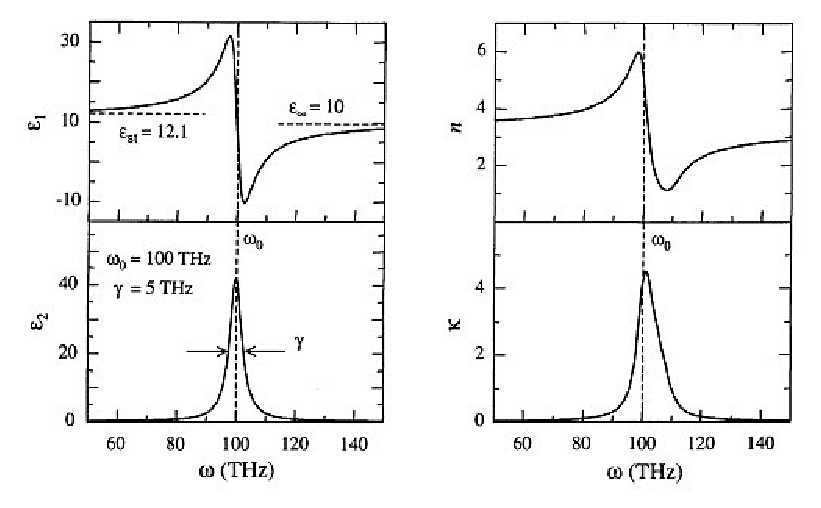
\includegraphics[width=0.6\textwidth]{24.eps}\\
  \label{fig:2.4}
\end{figure}\marginnote{Frequency dependence of the real and imaginary parts of the complex dielectric constant of a dipole oscillator at frequencies close to resonance. The graphs are calculated for an oscillator with $\omega_0=100$ THz, $\gamma=5$ THz, $\epsilon_{st}=12.1$ and $\epsilon_{\infty}=10$. (1 THz = $10^{12}$ Hz.) Also shown is the real and imaginary part of the refractive index calculated from the dielectric constant.}

and
\begin{equation}\label{equa:2.18}
  \epsilon_r(\infty)\equiv\epsilon_{\infty}=1+\chi
\end{equation}
respectively. The subscript on $\epsilon_{st}$ stands for 'static', since it represents the dielectric response to static electric fields. With this notation we find that:
\begin{equation}\label{equa:2.19}
  (\epsilon_{st}-\epsilon_{\infty})=\frac{Ne^2}{\epsilon_0m_0\omega_0^2}
\end{equation}
We finally rewrite eqns \ref{equa:2.15} and \ref{equa:2.16} in the following form valid at frequencies close to resonance:
\begin{eqnarray}
% \nonumber to remove numbering (before each equation)
  \epsilon_1(\Delta\omega) &=& \epsilon_{\infty}-(\epsilon_{st}-\epsilon_{\infty})\frac{2\omega_0\Delta\omega}{4(\Delta\omega)^2+\gamma^2}  \label{equa:2.20}\\
  \epsilon &=& (\epsilon_{st}-\epsilon_{\infty})\frac{\gamma\omega_0}{4(\Delta\omega)^2+\gamma^2} \label{equa:2.21}
\end{eqnarray}
These equations describe a sharp atomic absorption line centred at $\omega_0$ with full width at half maximum equal to $\gamma$.

Figure 2.4 shows the frequency dependence of $\epsilon_1$ and $\epsilon_2$ predicted by eqns \ref{equa:2.20}, \ref{equa:2.21} for an oscillator with $\omega_0 = 10^{14}$Hz, $\gamma = 5\times10^{12}$Hz, $\epsilon_{st}=12.1$ and $\epsilon_{\infty}=10$. These numbers are fairly typical of the infrared absorption lines in an ionic crystal. We see that $\epsilon_2$ is a strongly peaked function of $\omega$ with a maximum value at $\omega_0$ and a full width at half maximum equal to $\gamma$. The frequency dependence of $\epsilon_1$ is more complicated. As we approach $\omega_0$from below, $\epsilon_1$ gradually rises from the low frequency value of $\epsilon_{st}$, and reaches a peak at $\omega_0-\gamma/2$. (See Example 2.1.) It then falls sharply, passing through a minimum at $\omega_0+\gamma/2$ before rising again to the high frequency limit of $\epsilon_{\infty}$. Note that the frequency scale over which these effects occur is determined by $\gamma$ for both $\epsilon_1$ and $\epsilon_2$. This shows that the damping of the oscillator causes line broadening. The frequency dependence determined of $\epsilon_1$ and $\epsilon_2$ shown in Fig. 2.4 is called \textbf{Lorentzian} after the originator of the dipole model.

In an experiment we actually measure the refractive index $n$ and the absorption coefficient $\alpha$. The measurement of $\alpha$ then determines the extinction coefficient $\kappa$ through eqn \ref{equa:1.16}. Figure 2.4 shows the values of $n$ and $\kappa$ calculated from $\epsilon_1$ and $\epsilon_2$ using eqns \ref{equa:1.22} and \ref{equa:1.23}. We see that $n$ approximately follows the frequency dependence of $\sqrt{\epsilon_1(\omega)}$, while $\kappa$ more or less follows $\sqrt{\epsilon_2(\omega)}$. The correspondence $n\leftrightarrow\sqrt{\epsilon_1}$ and $\kappa\leftrightarrow\sqrt{\epsilon_2}$ would be exact if $\kappa$ were much smaller than $n$ (cf. eqns \ref{equa:1.24} and \ref{equa:1.25}). This is what generally happens in gases in which the low density of atoms makes the total absorption small. In the example shown in Fig. 2.4 the correspondence is only approximate because the absorption is very strong near $\omega_0$, so that we cannot always assume $n\gg\kappa$. Nevertheless, the basic behaviour shows that the absorption peaks at a frequency very close to $\omega_0$ and has a width of about $\gamma$, while the refractive index shows positive and negative excursions below and above $\omega_0$. This is the typical behaviour expected of an atomic absorption line.

One interesting aspect of the Lorentz oscillator is that it affects the refractive index over a much larger frequency range than the absorption. This point is clearly shown in the graphs given in Fig. 2.4. The absorption is a strongly peaked function of $\omega$ and falls off as $(\Delta\omega)^2$ as we tune away from resonance. Thus there is no significant absorption if we tune sufficiently far from resonance. On the other hand, the frequency dependence of the refractive index varies as $|\Delta\omega|^{-1}$ for large $|\Delta\omega|$. This follows from eqn \ref{equa:2.20} with the approximation $n=\sqrt{\epsilon_1}$, which is valid for large $|\Delta\omega|$ when $\epsilon_2$ is very small.

\begin{Exercise}
  The full width at half maximum of the strongest hyperfine component of the sodium D2 line at 589.0 nm is 100 MHz. A beam of light passes through a gas of sodium with an atom density of $1\times10^{17} \m^{-3}$. Calculate: (i) The peak absorption coefficient due to this absorption line. (ii) The frequency at which the resonant contribution to the refractive index is at a maximum. (iii) The peak value of the resonant contribution to the refractive index.
\end{Exercise}

\begin{Answer}
  (i) We are dealing with a low density gas of atoms, and so the approximations given in eqns \ref{equa:1.24} and \ref{equa:1.25} will be valid. This means that the absorption will directly follow the frequency dependence of $\epsilon_2(\omega)$, and the peak absorption will occur precisely at the line centre. The peak extinction coefficient can be worked out from eqns \ref{equa:2.16} and \ref{equa:1.25}. This gives:
  \begin{equation*}
    \kappa(\omega_0)=\frac{\epsilon_2(\omega_0)}{2n}=\frac{Ne^2}{2n\epsilon_0\omega_0}\frac{1}{\gamma\omega_0}
  \end{equation*}
  We do not know what $n$ is, but because we are dealing with a gas, it will only be very slightly different from unity. This point is confirmed in part (iii) of the question. We therefore take $n=1$ here, and insert $N=1\times10^{17}\m^{-3}$, $\gamma=2\pi\times100$ MHz and $\omega_0=2\pi c/\lambda=3.20\times10^{15}$ Hz, to find that $\kappa(\omega_0)= 7.90\times10^{-5}$. This confirms that $n\gg\kappa$, and hence that it is valid to use eqn \ref{equa:1.25}. We then work out the absorption coefficient from eqn \ref{equa:l.16}, which gives:
  \begin{equation*}
    \alpha_{max}=\alpha(\omega_0)=\frac{2\pi\kappa(\omega_0)}{\lambda}=1.7\times10^3\m^{-1}
  \end{equation*}
  \marginnote{The absorption coefficient measured in an experiment would actually be smaller than the value calculated here by about a factor of 3. This discrepancy is caused by the fact that we are assuming that the oscillator strength of the transition is unity. This point is discussed further in section 2.2.2 below.}

(ii) We know from Fig. 2.4 that there will be a peak in the refractive index just below $\omega_0$. Equation \ref{equa:1.24} tells us that $n(\omega)=\sqrt{\epsilon_1(\omega)}$, and hence that the local maximum of $n$ will occur at the same frequency as the maximum in $\epsilon_1$. Since the peak occurs near $\omega_0$, it will be valid to use eqn \ref{equa:2.20}. The local maximum occurs when:
\begin{equation*}
  \frac{d\epsilon_1(\omega)}{d\omega}=\frac{d\epsilon_1(\Delta\omega)}{d\Delta\omega}\propto\frac{4(\Delta\omega)^2-\gamma^2}{|4(\Delta\omega)^2+\gamma^2|^2}=0
\end{equation*}
\begin{figure}[htbp]
  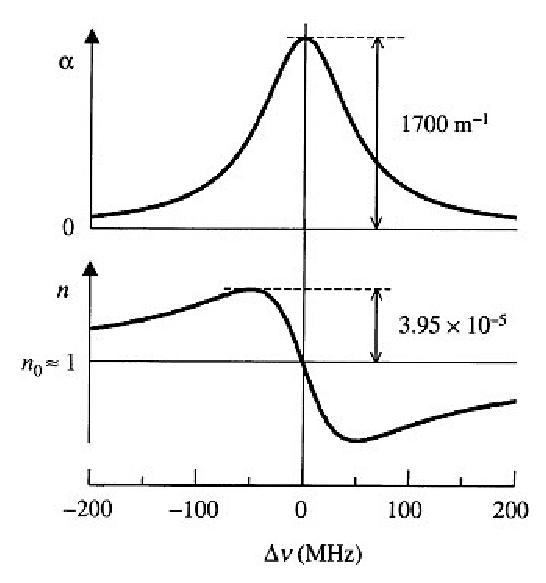
\includegraphics[width=0.4\textwidth]{25.eps}\\
  \label{fig:2.5}
\end{figure}\marginnote{Absorption coefficient and refractive index of sodium gas in the vicinity of the strongest hyperfine component of the D1 line, on the assumption that the oscillator strength of the transition is unity, and that the atom density is $1\times10^{17}\m^{-3}$. See Example 2.1 for the details. no represents the off-resonant refractive index, which is approximately equal to unity.}
This gives $\Delta\omega=\pm\gamma/2$. We see from Fig. 2.4 that $\Delta\omega=-\gamma/2$ corresponds to the local maximum, while $\Delta\omega=+\gamma/2$ corresponds to the local minimum. Therefore the peak in the refractive index occurs 50 MHz below the line centre.

(iii) From part (ii) we know that the local maximum in the refractive index occurs when $\Delta\omega=-\gamma/2$. We see from eqns \ref{equa:1.24} and \ref{equa:2.20} that the refractive index at this frequency is given by:
\begin{equation*}
  n_{max}=\sqrt{\epsilon_1}=\left(\epsilon_{\infty}+\frac{Ne^2}{2\epsilon_0m_0\omega_0\gamma}\right)^{\frac{1}{2}}=n_0\left(1+\frac{7.90\times10^{-5}}{n_0^2}\right)^{\frac{1}{2}}
\end{equation*}
where $n_0=\sqrt{\epsilon_{\infty}}$ is the off-resonant refractive index. We are dealing with a low density gas, and so it is justified to take $n_0\approx1$ here. This implies that the peak value of the resonant contribution to the refractive index is $3.95\times 10^{-5}$.

The full frequency dependence of the absorption and refractive index near this absorption line is plotted in Fig. 2.5.
\end{Answer}

\subsection{Multiple resonances}

In general, an optical medium will have many characteristic resonant frequencies. We already discussed in Section 2.1 how we expect to observe separate resonances due to the lattice vibrations and to the oscillations of the bound electrons within the atoms. Furthermore, a particular medium may have many resonances of each type. We can treat these multiple resonances without difficulty in our model provided they occur at distinct frequencies.

In writing eqn \ref{equa:2.12} we split the polarization of the medium into a resonant part and a non-resonant part. We then discussed the resonant part in detail, without specifying very accurately what we meant by the non-resonant term. We simply stated that $\mathrm{P}$ was proportional to $\vec{\varepsilon}$ through the susceptibility $\chi$. In reality, the non-resonant polarization of the medium must originate from the polarizability of the atoms in exactly the same way as the resonant part. Equation \ref{equa:2.19} tells us that the dielectric constant decreases each time we go through an absorption line. The contributions that enter the background electric susceptibility $\chi$ in eqn \ref{equa:2.12} thus arise from the polarization due to all the other oscillators at higher frequencies.

We can understand this point better by making it more quantitative. The contribution to the polarization of a particular oscillator is given by eqn \ref{equa:2.10}. In a medium with many electronic oscillators of different frequencies, the total polarization will therefore be given by
\begin{equation}\label{equa:2.22}
  \mathrm{P}=\left(\frac{Ne^2}{m_0}\sum_j\frac{1}{(\omega_j^2-\omega^2-i\gamma_j\omega)}\right)\vec{\varepsilon}
\end{equation}
where $\omega_j$ and $\gamma_j$ are the frequency and damping terms of a particular resonance line. We then substitute this into eqn \ref{equa:2.11}, and recall the definition of $\varepsilon_r$ given in eqn \ref{equa:2.13}. This gives:
\begin{equation}\label{equa:2.23}
  \epsilon_r(\omega)=1+\frac{Ne^2}{\epsilon_0m_0}\sum_j\frac{1}{(\omega_j^2-\omega^2-i\gamma_j\omega)}
\end{equation}
This equation takes account of all the transitions in the medium and can be used to calculate the full frequency dependence of the dielectric constant.

The refractive index and absorption coefficient calculated from eqn \ref{equa:2.23} are plotted against frequency in Fig. 2.6. The figure has been calculated for a hypothetical solid with three well-separated resonances with $\omega_j$ equal to $4\times 10^{13}$Hz, $4\times10^{15}$Hz and $1\times10^{17}$Hz respectively. The width of each absorption line has been set to $10\%$ of the centre frequency by appropriate choice of the damping term. The resonance in the infrared is included to represent the vibrational absorption. In a real solid, we would have to adapt the model appropriately to account for the different reduced mass and effective charge of the vibrational oscillator.

We can understand this figure by starting at the highest frequencies and gradually working our way down to the lower frequencies. At the very highest frequencies, the electrons are incapable of responding to the driving field. The medium therefore has no polarization, and the dielectric constant is unity. As we reduce the frequency, we first run into the transitions of the inner electrons in the X-ray/vacuum-ultraviolet spectral region, and then the transitions of the outer electrons in the ultraviolet and visible. We then have a region with no transitions until we finally reach the vibrational frequencies in the infrared. Each time we go through one of these resonances, we see the characteristic frequency dependence of the Lorentz oscillator, with a peak in the absorption spectrum and a `wiggle' in the refractive index. In between the resonances the medium is transparent: the absorption coefficient is zero and the refractive index is almost constant.
\begin{figure}[htbp]
  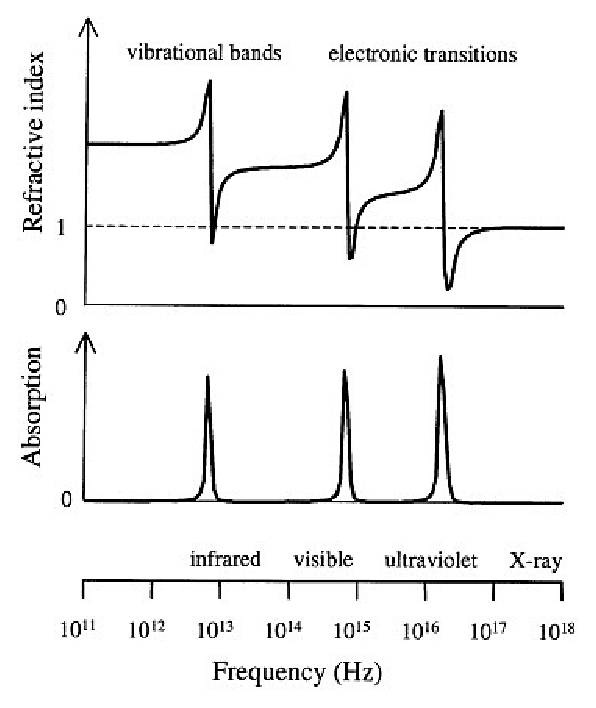
\includegraphics[width=0.4\textwidth]{26.eps}\\
  \label{fig:2.6}
\end{figure}\marginnote{Schematic diagram of the frequency dependence of the refractive index and absorption of a hypothetical solid from the infrared to the X-ray spectral region. The solid is assumed to have three resonant frequencies with $\omega_j=4\times10^{13}$ Hz, $4\times10^{15}$ Hz and $l\times10^{17}$ Hz respectively. The width of each absorption line has been set to $10\%$ of the centre frequency by appropriate choice of the $\gamma_j$'s.}


The value of the refractive index in the transparent regions gradually increases as we go through more and more resonance lines on decreasing the frequency. This increase of the refractive index is caused by the fact that $\epsilon_{st}>\epsilon_{\infty}$ (cf. eqn \ref{equa:2.19}), which implies that n is larger below an absorption line than above it. By reference to Fig. 2.6, we now see that we have to understand `static' and `$\infty$' as relative to a particular resonance. The variation of $n$ with frequency due to the resonances is the origin of the dispersion found in optical materials even when they are transparent. This point will be discussed further in Section 2.3 below.\marginnote{An astute reader will have noticed that the peak absorption coefficient for the three transition lines shown in Fig. 2.6 decreases slightly with decreasing frequency. This happens because n is larger at the lower frequencies. The transitions all have the same peak $\epsilon_2$, but we can see from eqn \ref{equa:1.21} that $\kappa$ must be slightly smaller if $n$ is larger.}

The dipole oscillator model predicts that each oscillator contributes a term given by eqn \ref{equa:2.10}. This leads to a series of absorption lines of the same strength. However, experimental data shows that the absorption strength actually varies considerably between different atomic transitions. With the benefit of hindsight, we know that this is caused by the variation of the quantum mechanical transition probability. (See Appendix B.) In classical physics, however, there is no explanation, and we just assign a phenomenological \textbf{oscillator strength} $f_j$ to each transition, rewriting eqn \ref{equa:2.23} as:
\begin{equation}\label{equa:2.24}
  \epsilon_r(\omega)=1+\frac{Ne^2}{\epsilon_0m_0}\sum_j\frac{f_j}{\omega_{0j}^2-\omega^2-i\gamma_j\omega}
\end{equation}
It can be shown from quantum mechanics that we must have $\sum_jf_j=1$ for each electron. Since the classical model predicts $f_j = 1$ for each oscillator, we then interpret this by saying that a particular electron is involved in several transitions at the same time, and the absorption strength is being divided between these transitions.

\subsection{Comparison with experimental data}

The schematic behaviour shown in Fig. 2.6 can be compared to experimental data on a typical solid state material. Figure 2.7 shows the frequency dependence of the refractive index and extinction coefficient of fused silica ($\mathrm{SiO_2}$) glass from the infrared to the X-ray spectral region. The general characteristics indicated by Fig. 2.6 are clearly observed, with strong absorption in the infrared and ultraviolet, and a broad region of low absorption in between. The data confirms that $n\gg\kappa$ except near the peaks of the absorption. This means that the approximation whereby we associate the frequency dependence of $n$ with that of $\epsilon_1$, and that of $\kappa$ with $\epsilon_2$ (eqns \ref{equa:1.24} and \ref{equa:1.25}), is valid at most frequencies.

The general behaviour shown in Fig. 2. 7 is typical of optical materials which are transparent in the visible spectral region. We already noted in Sections 1.4.1 and 1.4.2 that the transmission range of colourless materials is determined by the electronic absorption in the ultraviolet and the vibrational absorption in the infrared. This is demonstrated by the transmission data for sapphire shown in Fig. 1.4(a).

\begin{figure}[htbp]
  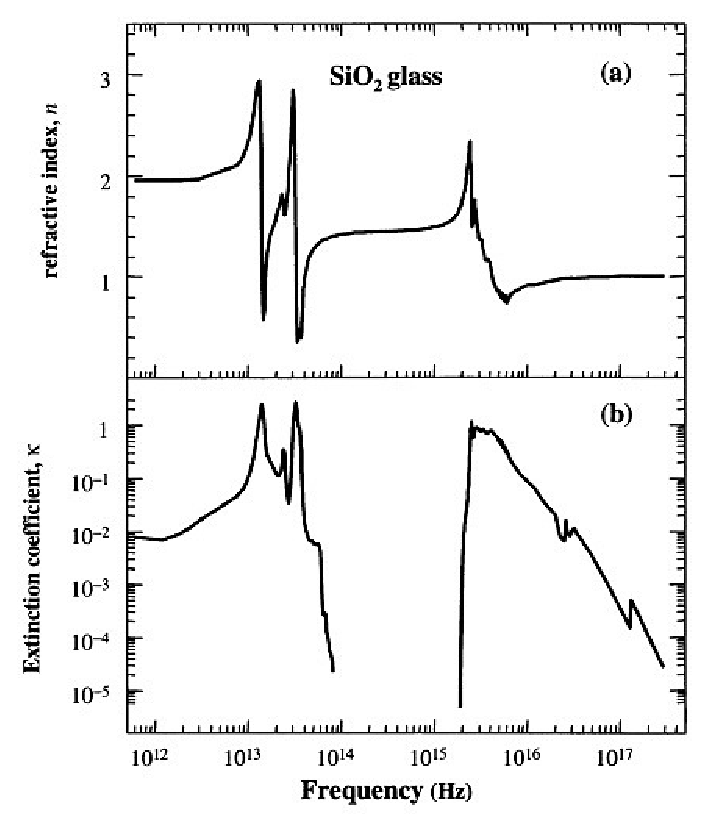
\includegraphics[width=0.4\textwidth]{27.eps}\\
  \label{fig:2.7}
\end{figure}\marginnote{(a) Refractive index and (b) extinction coefficient of fused silica ($\mathrm{SiO_2}$) glass from the infrared to the x-ray spectral region.}

Silica is a glass, and hence does not have a regular crystal lattice. The infrared absorption is therefore caused by excitation of vibrational quanta in the $\mathrm{SiO_2}$ molecules themselves. Two distinct peaks are observed at $1.4\times10^{13}$Hz ($21\mu m$) and $3.3\times10^{13}$Hz ($9.1\mu m$) respectively. These correspond to different vibrational modes of the molecule. The detailed modeling of these absorption bands by the oscillator model will be discussed in Chapter \ref{chap:10}.

The ultraviolet absorption in silica is caused by interband electronic transitions. $\mathrm{SiO_2}$ has a fundamental band gap of about $\mathrm{10 eV}$, and interband transitions are possible whenever the photon energy exceeds this value. Hence we observe an absorption threshold in the ultraviolet at $\mathrm{2\times10^{15}Hz (150nm)}$. The interband absorption peaks at around $3\times10^{15}$Hz with an extremely high absorption coefficient of $\sim10^8 m^{-1}$, and then gradually falls off to higher frequency. Subsidiary peaks are observed at $\sim3\times 10^{16}$Hz and $1.3\times10^17$Hz. These are caused by transitions of the inner core electrons of the silicon and oxygen atoms. The fact that the electronic absorption consists of a continuous band rather than a discrete line makes it hard to model accurately as a Lorentz oscillator. We will discuss the quantum theory of the interband absorption in Chapter \ref{chap:3}.

The refractive index of glass has resonances in the infrared and the ultraviolet which correspond to the interband and vibrational absorption. In the far infrared region below the vibrational resonance, the refractive index is $\sim2$, while in the hard ultraviolet and X-ray region it approaches unity. In the transparency region between the vibrational and interband absorption, the refractive index has a value of $\sim1.5$. Closer inspection of Fig. 2.7 shows that the refractive index actually increases with frequency in this transparency region, rising from a value of 1.40 at $8\times 10^{13}$Hz ($3.5\mu m$) to 1.55 at $1.5\times10^{15}$Hz (200 nm). This dispersion originates from the low frequency wings of the ultraviolet absorption and the high frequency wings of the infrared absorption, and will be discussed in more detail in Section 2.3 below.

The data in Fig. 2.7 show that the refractive index falls below unity at a number of frequencies. This implies that the phase velocity of the light is greater than $c$, which might seem to imply a contradiction with relativity. However, this overlooks the fact that a signal must be transmitted as a wave packet rather than as a monochromatic wave. In a dispersive medium, a wave packet will propagate at the \textbf{group velocity} $v_g$ given by:
\begin{equation}\label{equa:2.25}
  v_g=\frac{d\omega}{dk}
\end{equation}
rather than at the phase velocity $v = \omega/ k = c/n$. The relationship between $v_g$ and $v$ is:\marginnote{It is apparent from Fig. 2.6 that $dn/dk$ will be negative at some frequencies close to one of the resonance lines. Equation \ref{equa:2.26} then implies that $v_g > v$, and so we could again run into a problem with relativity. However, the medium is highly absorbing in these frequency regions, and this means that the signal travels with yet another velocity called the signal velocity. This is always less than $c$.}
\begin{equation}\label{equa:2.26}
  v_g=v\left(1-\frac{k}{n}\frac{dn}{dk}\right)
\end{equation}
The derivation of this result is left as an exercise to the reader. (See Exercise 2.7.) We will see in Section 2.3 that $dn/dk$ is positive in most materials at optical frequencies. This then implies that $v_g$ is always less than $v$, and if we were to try to transmit a signal in a spectral region where $v > c$, we would always find that $v_g$ is less than $c$. The proof of this for a simple Lorentz oscillator is considered in Exercise 2.8.

\subsection{Local field corrections}

\marginnote{
\begin{minipage}{\textwidth}
    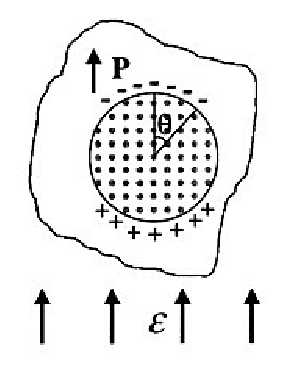
\includegraphics[width=25mm]{28.eps}
    \label{fig:2.8}
  \end{minipage}
 \\ [\intextsep]
Model used to calculate the local field by the Lorentz correction. An imaginary spherical surface drawn around a particular atom divides the medium into nearby dipoles and distant dipoles. The field at the centre of the sphere due to the nearby dipoles is summed exactly, while the field due to the distant dipoles is calculated by treating the material outside the sphere as a uniformly polarized dielectric.}

The calculation of the dielectric constant given in eqn \ref{equa:2.24} is valid in a rarefied gas with a low density of atoms. However, in a dense optical medium such as a solid, there is another factor that we must consider. The individual atomic dipoles respond to the local field that they experience. This may not necessarily be the same as the external field, because the dipoles themselves generate electric fields which will be felt by all the other dipoles. The actual local field experienced by an atom therefore takes the form:
\begin{equation}\label{equa:2.27}
  \vec{\varepsilon}_{local}=\vec{\varepsilon}+\vec{\varepsilon}_{other dipoles}
\end{equation}
where $\vec{\varepsilon}$ and $\vec{\varepsilon}_{other}$ dipoles represent the fields due to the external field and the other dipoles respectively. We should have been using $\vec{\varepsilon}_{local}$ instead of $\vec{\varepsilon}$ all along throughout the calculation given in Sections 2.2.1 and 2.2.2.

The calculation of the correction field due to the other dipoles in the medium is actually a rather complicated one. An approximate solution due to Lorentz can be derived if we assume that all the dipoles are parallel to the applied field and are arranged on a cubic lattice. The calculation works by separating the contribution from the nearby dipoles and that from the rest of the sample, as indicated in Fig. 2.8. The division is effected by an imaginary spherical surface with a radius large enough to make it sensible to average the material outside it. The problem is then reduced to summing the field of the dipoles inside the sphere at the one in the middle, and then calculating the effect of a uniformly polarized dielectric outside the sphere. The final result is:
\begin{equation}\label{equa:2.28}
  \vec{\varepsilon}_{other dipoles}=\frac{\mathrm{P}}{3\epsilon_0}
\end{equation}
where $\mathrm{P}$ is the polarization of the dielectric outside the sphere. The derivation of this result is the subject of Exercise 2.9. By using the result of eqn \ref{equa:2.28} in eqn \ref{equa:2.27} we find that:
\begin{equation}\label{equa:2.29}
  \vec{\varepsilon}_{local}=\vec{\varepsilon}+\frac{\mathrm{P}}{3\epsilon_0}
\end{equation}
The macroscopic polarization $\mathrm{P}$ will be given by
\begin{equation}\label{equa:2.30}
  \mathrm{P}=N\epsilon_0\chi_a\varepsilon_{local}
\end{equation}
where $\chi_a$ is the electric susceptibility per atom. $\chi_a$ is defined by:
\begin{equation}\label{equa:2.31}
  \mathrm{p}=\epsilon_0\chi_a\varepsilon_{local}
\end{equation}
$\mathrm{p}$ being the induced dipole moment per atom. This is analogous to the usual definition of the macroscopic susceptibility given in eqn A.l, except that it is now applied to individual atoms interacting with the local field. We can see from eqn \ref{equa:2.10} that $\chi_a$ is given by
\begin{equation}\label{equa:2.32}
  \chi_a=\frac{e^2}{\epsilon_0m_0}\frac{1}{(\omega_0^2-\omega^2-i\gamma\omega)},
\end{equation}
if there is just a single resonance. This is modified to
\begin{equation}\label{equa:2.33}
  \chi_a=\frac{e^2}{\epsilon_0m_0}\sum_j\frac{f_j}{(\omega_j^2-\omega^2-i\gamma_j\omega)}
\end{equation}
if there are multiple resonances (cf. eqn \ref{equa:2.24}).

We can combine eqns \ref{equa:2.29} and \ref{equa:2.30} with eqns \ref{equa:2.11} and \ref{equa:2.13} by writing
\begin{equation}\label{equa:2.34}
  \mathrm{P}=N\epsilon_0\chi_a\left(\vec{\varepsilon}+\frac{\mathrm{P}}{3\epsilon_0}\right)=(\epsilon_r-1)\epsilon_0\vec{\varepsilon}
\end{equation}
We put all this together to find that:
\begin{equation}\label{equa:2.35}
  \frac{\epsilon_r-1}{\epsilon_r+2}=\frac{N\chi_a}{3}
\end{equation}
This result is known as the \textbf{Clausius-Mossotti relationship}. The relationship works well in gases and liquids. It is also valid for those crystals in which the Lorentz correction given in eqn \ref{equa:2.29} gives an accurate account of the local field effects, namely cubic crystals.

\subsection{The Kramers-Kronig relationships}

The discussion of the dipole oscillator shows that the refractive index and the absorption coefficient are not independent parameters but are related to each other. This is a consequence of the fact that they are derived from the real and imaginary parts of a single parameter, namely the complex refractive index. If we invoke the law of causality (that an effect may not precede its cause) and apply complex number analysis, we can derive general relationships between the real and imaginary parts of the refractive index. These are known as the \textbf{Kramers-Kronig} relationships and may be stated as follows:
\begin{eqnarray}
% \nonumber to remove numbering (before each equation)
  n(\omega) &=& 1+\frac{1}{\pi}\texttt{P}\int_{-\infty}^{\infty}\frac{\kappa(\omega')}{\omega'-\omega}d\omega' \\
  \kappa(\omega) &=& -\frac{1}{\pi}\texttt{P}\int_{-\infty}^{\infty}\frac{n(\omega')-1}{\omega'-\omega}d\omega'
  \end{eqnarray}
where $\texttt{P}$ indicates that we take the principal part of the integral.

The Kramers-Kronig relationships allow us to calculate $n$ from $\kappa$, and \textit{vice versa}. This can be very useful in practice, because it would allow us, for example, to measure the frequency dependence of the optical absorption and then calculate the dispersion without needing to make a separate measurement of $n$.

\section{Dispersion}

Figure 2.9 plots the refractive index data from Fig. 2.7 in more detail. The data show that the refractive index increases with frequency in the near infrared and visible spectral regions. We have seen in Section 2.2.3 that this dispersion originates mainly from the interband absorption in the ultraviolet. At visible frequencies the absorption from these transitions is negligible and the glass is transparent. However, the ultraviolet absorption still affects the refractive index through the extreme wings of the Lorentzian line. In the near infrared, the dispersion is also affected by the high frequency wings of the vibrational absorption at lower frequency.
\begin{figure}[htbp]
  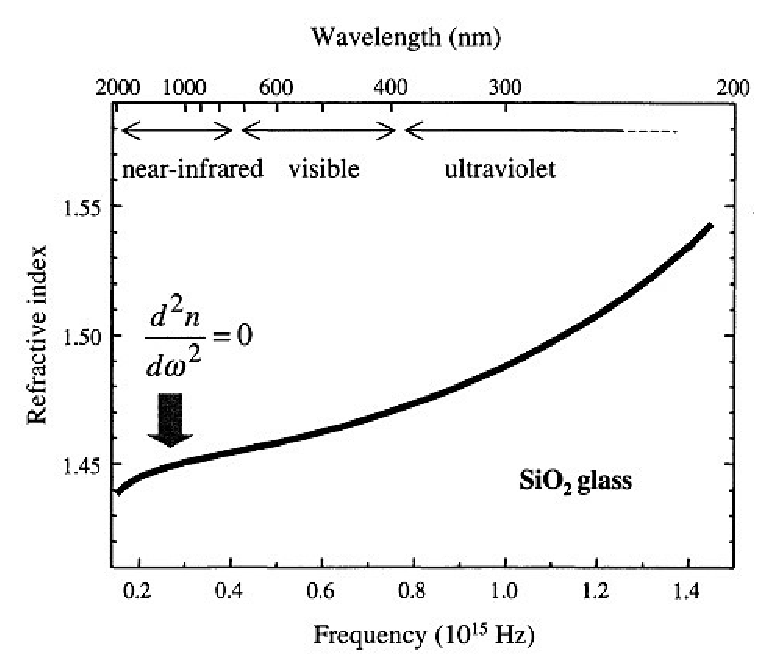
\includegraphics[width=0.4\textwidth]{29.eps}\\
  \label{fig:2.9}
\end{figure}\marginnote{Refractive index of $\mathrm{SiO_2}$ glass in the near infrared, visible and ultraviolet spectral regions.}

A material in which the refractive index increases with frequency is said to have \textbf{normal} dispersion, while one in which the contrary occurs is said to have \textbf{anomalous} dispersion. A number of empirical formulae to describe the normal dispersion of glasses have been developed over the years. (See Exercise 2.12.)\marginnote{The use of the words `normal' and `anomalous' is somewhat misleading here. The dipole oscillator model shows us that all materials have anomalous dispersion at some frequencies. The phraseology was adopted before measurements of the refractive index had been made over a wide frequency range and the origin of dispersion had been properly understood.}

The dispersion of the refractive index of glasses such as silica can be used to separate different wavelengths of light with a prism, as shown in Fig. 2.10. The blue light is refracted more because of the higher index of refraction, and is therefore deviated through a larger angle by the prism. (See Exercise 2.13.) This effect is used in prism spectrometers.

One of the effects of dispersion is that light of different frequencies takes a different amount of time to propagate through a material. (See Exercise 1.11, for example.) A pulse of light of duration $t_p$ must necessarily contain a spread of frequencies given approximately by
\marginnote{
\begin{minipage}{\textwidth}
    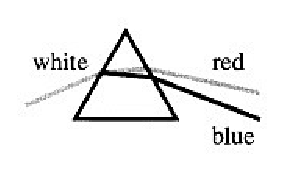
\includegraphics[width=25mm]{210.eps}
    \label{fig:2.10}
  \end{minipage}
 \\ [\intextsep]
Separation of white light into different colours by dispersion in a glass prism.}

\begin{equation}\label{equa:2.38}
  \Delta v\approx\frac{1}{t_p}
\end{equation}
in order to satisfy the 'uncertainty principle' $\Delta v\Delta t\sim 1$. Dispersion will therefore cause the pulse to broaden in time as it propagates through the medium. This can become a serious problem when attempting to transmit very short pulses through a long length of an optical material, for example in a high speed optical fibre telecommunications system.

We mentioned in Section 2.2.3 that a pulse of light travels with the group velocity $v_g$. The important parameter for pulse spreading due to dispersion is therefore the \textbf{group velocity dispersion} (\textbf{GVD}) (see Exercise 2.14):
\begin{equation}\label{equa:2.39}
  GVD=\frac{d^2\omega}{dk^2}\approx\frac{d^2n}{d\omega^2}\approx\frac{d^2n}{d\lambda^2}
\end{equation}
The Lorentz model indicates that the GVD is positive below an absorption line and negative above it. Applying this to the data in Fig. 2.9, we see negative GVD in the infrared due to the vibrational absorption and positive GVD in the visible due to the interband absorption in the ultraviolet. These two effects cancel at a wavelength in the near infrared which is identified in Fig. 2.9. This region of zero GVD occurs around $\mathrm{1.3\mu m}$ in silica optical fibres. Short pulses can be transmitted down the fibre with negligible temporal broadening at this wavelength, and so it is one of the preferred wavelengths for optical fibre communication systems.

\section{Optical Anisotropy: Birefringence}

The atoms in a solid are locked into a crystalline lattice with well defined axes. In general, we cannot assume that the optical properties along the different crystalline axes are equivalent. For example, the separation of the atoms might not be the same in all directions. This would lead to different vibrational frequencies, and hence a change in the refractive index between the relevant directions. This optical anisotropy contrasts with gases and liquids which are isotropic because the atoms have no preferred directions ih the absence of external perturbations such as applied magnetic or electric fields.

Optical anisotropy gives rise to the phenomenon of \textbf{birefringence}. We can describe the properties of a birefringent crystal by generalizing the relationship between the polarization and the applied electric field. If the electric field is applied along an arbitrary direction relative to the crystalline axes, we must write a tensor equation to relate $\mathrm{P}$ to $\vec{\varepsilon}$:\marginnote{Equation \ref{equa:2.40} should be contrasted with the usual scalar relationship between $\mathbf{P}$ and $\vec{\varepsilon}$ namely (cf. eqn A.l):
\begin{equation*}
  \mathbf{P}=\epsilon_0\chi\vec{\varepsilon}
\end{equation*}
which only applies to isotropic materials.}
\begin{equation}\label{equa:2.40}
  \mathrm{P}=\epsilon_0\vec{\chi}\vec{\varepsilon}
\end{equation}
where $\vec{\chi}$ represents the susceptibility tensor. Written explicitly in terms of the components, we have:
\begin{equation}\label{equa:2.41}
\left(  \begin{array}{c}
    P_x \\
    P_y \\
    P_z \\
  \end{array}
\right)=\epsilon_0\left(
                    \begin{array}{ccc}
                      \chi_{11} & \chi_{12} & \chi_{13} \\
                      \chi_{21} & \chi_{22} & \chi_{23} \\
                      \chi_{31} & \chi_{32} & \chi_{33} \\
                    \end{array}
                  \right)\left(
                           \begin{array}{c}
                             \varepsilon_x \\
                             \varepsilon_y \\
                             \varepsilon_z \\
                           \end{array}
                         \right)
                         \end{equation}
We can simplify this by choosing the cartesian coordinates $x$, $y$, and $z$ to correspond to the principal crystalline axes. In this case, the off-diagonal components are zero, and the susceptibility tensor takes the form:
\begin{equation}\label{equa:2.42}
  \vec{\chi}=\left(
                  \begin{array}{ccc}
                    \chi_{11} & 0 & 0 \\
                    0 & \chi_{22} & 0 \\
                    0 & 0 & \chi_{33} \\
                  \end{array}
                \right)
\end{equation}
The relationships between the components are determined by the crystal symmetry.

\begin{table}[htdp]\scriptsize
%%\caption{Refractive indices of some common uniaxial crystals at 589.3 nm.}
\begin{tabular}{cccccc}\label{tab:2.1}

  % after \\:   or \cline{col1-col2} \cline{col3-col4} ...
  Crystal & Chemical structure & Symmetry class & type & $n_0$ & $n_e$\\

  Ice & $\mathrm{H_2O}$ & trigonal & positive & 1.309 & 1.313 \\
  Quartz & $\mathrm{SiO_2}$ & trigonal & positive & 1.544 & 1.553 \\
  Beryl & $\mathrm{Be_3Al_2(SiO_3)_6}$ & hexagonal & negative & 1.581 & 1.575 \\
  Sodium nitrate & $\mathrm{NaNO_3}$ & trigonal & negative & 1.584 & 1.336 \\
  Calcite & $\mathrm{CaCO_3}$ & trigonal & negative & 1.658 & 1.486 \\
  Tourmaline & complex silicate & trigonal & negative & 1.669 & 1.638 \\
  Sapphire & $\mathrm{Al_2O_3}$ & trigonal & negative & 1.768 & 1.760 \\
  Zircon & $\mathrm{ZrSiO_4}$ & tetragonal & positive & 1.923 & 1.968 \\
  Rutile & $\mathrm{TiO_2}$ & tetragonal & positive & 2.616 & 2.903 \\

\end{tabular}
\end{table}

\begin{figure}
  \centering
  % Requires \usepackage{graphicx}
  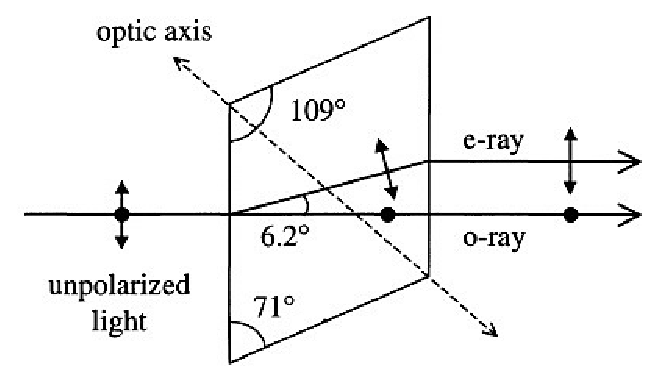
\includegraphics[width=0.6\textwidth]{211.eps}\\
  \label{fig:2.11}
\end{figure}\marginnote{Double refraction in a natural calcite crystal. The shape of the crystal and the orientation of the optic axis is determined by the cleavage planes of calcite. An unpolarized incident light ray is split into two spatially separated orthogonally polarized rays. The $\bullet$ symbol for the o-ray indicates that it is polarized with its field pointing out of the page.}


\begin{itemize}
  \item In cubic crystals, the $x$, $y$ and $z$ axes are indistinguishable. \marginnote{Crystals with cubic symmetry are only isotropic as regards their linear optical properties. We will see in Chapter \ref{chap:11} that cubic crystals can actually have anisotropic nonlinear optical properties.}They therefore have $\chi_{11}=\chi_{22}=\chi_{33}$, and their optical properties are isotropic.
  \item Crystals with tetragonal, hexagonal or trigonal (rhombohedral) symmetry are called \textbf{uniaxial} crystals. These crystals possess a single \textbf{optic axis}, which is usually taken as the $z$ axis. In hexagonal crystals, for example, the optic axis is defined by the direction normal to the plane of the hexagons. The optical properties are the same along the $x$ and $y$ directions, but not along the $z$ direction. This implies that $\chi_{11}=\chi_{22}=\chi_{33}$. Some examples of uniaxial crystals are listed in Table 2.1.
  \item Crystals with orthorhombic, monoclinic or triclinic symmetry are called \textbf{biaxial} crystals. They have two optic axes, and all three diagonal components of the susceptibility tensor are different. Mica is an important example of a biaxial crystal, since it is widely used for making optical wave plates.
\end{itemize}

One very striking demonstration of optical anisotropy is the phenomenon of \textbf{double refraction}. In this effect an unpolarized light ray is separated into two rays which emerge displaced from each other, as shown in Fig. 2.11. These two rays are called `ordinary' and `extraordinary', and are orthogonally polarized to each other.

\begin{figure}
  \centering
  % Requires \usepackage{graphicx}
  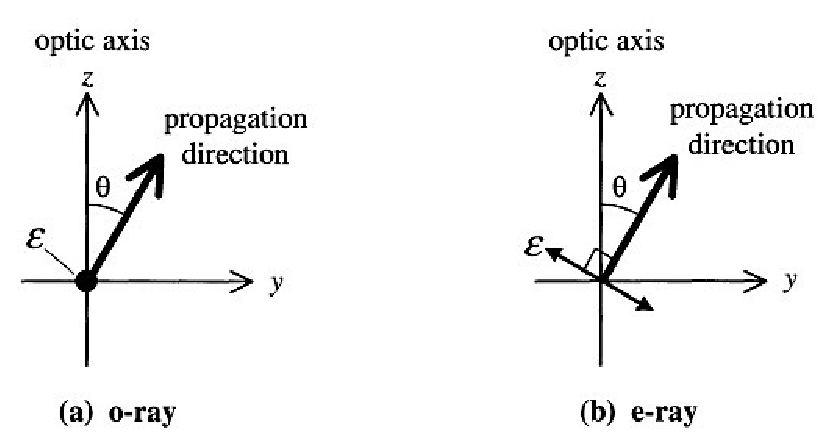
\includegraphics[width=0.6\textwidth]{212.eps}\\
  \label{fig:2.12}
\end{figure}
\marginnote{Electric field vector of ray propagating in a uniaxial crystal with its optic axis along the $z$ direction. The ray makes an angle of $\theta$ with respect to the optic axis. The $x$ and $y$ axes are chosen so that the beam is propagating in the $y$, $z$ plane. The polarization can be resolved into: (a) a component along the $x$ axis and (b) a component at an angle of $90^\circ-\theta$ to the optic axis. (a) is the o-ray and (b) is the e-ray.}

The phenomenon of double refraction can be explained by assuming that the crystal has different refractive indices for the orthogonal polarizations of the ordinary and extraordinary rays. These two refractive indices are usually labelled $n_o$ and $n_e$ respectively. Consider the propagation of a beam of unpolarized light which enters a uniaxial crystal at an angle $\theta$ to the optic axis, which is taken to lie along the $z$ axis. The optical properties are isotropic in the $x$, $y$ plane, and so we can choose the axes so that the beam is propagating in the $y$, $z$ plane without loss of generality, as shown in Fig. 2.12. This allows us to split the polarization of the light into two orthogonal components, one of which is polarized along the $x$ axis, and the other polarized at an angle of $(90^\circ-\theta)$ to the optic axis. The former is the o(rdinary)-ray, and the latter is the e(xtraordinary)-ray. Now the refractive index will be different for light which is polarized along the $z$ axis or in the $x$, $y$ plane. Therefore the o-ray experiences a different refractive index to the e-ray, and will thus be refracted differently: hence double refraction. On the other hand, if the beam propagates
along the optic axis so that $\theta = 0$, the $\vec{\varepsilon}$ vector of the light will always fall in
the $x$, $y$ plane. In this case, no double refraction will be observed because the $x$ and $y$ directions are equivalent and there is no e-ray.

Double refraction was first observed in natural uniaxial crystals such as calcite ('Iceland Spar') and quartz. Table 2.1 lists the refractive indices for the o- and e-rays of calcite and quartz, together with those of several other uniaxial crystals. The birefringent crystals are classified as being either positive or negative depending on whether $n_e$ is greater or smaller than $n_o$ .

Further discussion of the detailed effects of birefringence can be found in most optics textbooks. The purpose of introducing birefringence here is to give an example of how the phenomenon of optical anisotropy arises from the underlying symmetry of the crystal structure. This is a very standard example of an optical effect that occurs in crystalline solids and is not found in gases or liquids.
\begin{Exercise}
  The optic axis of a uniaxial crystal lies along the $z$ axis. The refractive index for light polarized in the $z$ direction is $n_e$, while that for light polarized in the $x$, $y$ plane is $n_o$. Write down the dielectric constant tensor defined  through the tensor relationship
  \begin{equation*}
    \mathbf{D}=\epsilon_0\epsilon_r\vec{\varepsilon}
  \end{equation*}
\end{Exercise}
\begin{Answer}
  We make use of eqns \ref{equa:2.11} and \ref{equa:2.40} to write:
  \begin{eqnarray}
  % \nonumber to remove numbering (before each equation)
\nonumber   \mathbf{D} &=& \epsilon_0\vec{\varepsilon}+\mathbf{P} \\
\nonumber     &=&      \epsilon_0\vec{\varepsilon}+\epsilon_0\chi\vec{\varepsilon} \\
     &=& \epsilon_0(1+\chi)\vec{\varepsilon}\equiv\epsilon_0\epsilon_r\vec{\varepsilon} \label{equa:2.43}
  \end{eqnarray}
  Hence we see that:
  \begin{equation}\label{equa:2.44}
    \epsilon_r=1+\chi
  \end{equation}
  The susceptibility tensor is given by eqn \ref{equa:2.42}, and hence the dielectric constant tensor will take the form:
\begin{equation}\label{equa:2.45}
  \epsilon_r=\left(
    \begin{array}{ccc}
      1+\chi_{11} & 0 & 0 \\
      0 & 1+\chi_{22} & 0 \\
      0 & 0 & 1+\chi_{33} \\
    \end{array}
  \right)
\end{equation}
In a uniaxial crystal with the optic axis along the z direction, we must have $\chi_{11}=\chi_{22}\ne\chi_{33}$.

We now further assume that the crystal is transparent, so that the dielectric constant is just equal to the square of the refractive index (cf. eqns \ref{equa:1.24} and \ref{equa:1.25} with $\kappa=0$). If we had a linearly polarized light beam with the electric field directed along the $x$ or $y$ directions, we would measure a refractive index of $n_o$. This tells us that:
\begin{equation*}
  1+\chi_{11}=1+\chi_{22}=n_o^2
\end{equation*}
On the other hand, if $\vec{\varepsilon}$ is along the $z$ axis, we would measure a refractive index of $n_e$, which implies that
\begin{equation*}
  1+\chi_{33}=n_e^2
\end{equation*}
Therefore the dielectric constant tensor must be:
\begin{equation}\label{equa:2.46}
  \epsilon_r=\left(
               \begin{array}{ccc}
                 n_o^2 & 0 & 0 \\
                 0 & n_o^2 & 0 \\
                 0 & 0 & n_e^2 \\
               \end{array}
             \right)
\end{equation}
\end{Answer}

\section*{Chapter  Summary}

\definecolor{shadecolor}{rgb}{1,0.9,0.9}
\begin{shaded}
\begin{itemize}
  \item The classical model of a solid treat the atoms and molecules as oscillating electric dipoles with characteristic resonant frequencies. The resonances due to the bound electrons occur in the near infrared, visible and ultraviolet spectral regions ($10^{14}-10^{15}$Hz), while those associated with vibrations occur in the infrared ($10^{12}-10^{13}$Hz). Free electrons can be treated in the dipole oscillator model by assuming that the natural resonant frequency is 0.
  \item The medium absorbs light when the frequency coincides with one of its resonant frequencies. In non-resonant conditions, the medium is transparent, but the velocity of light is reduced by multiple coherent elastic scattering.
  \item The absorption coefficient of an individual dipole oscillator has a Lorentzian line shape (cf. eqn \ref{equa:2.21}). The spectral width of the absorption line is equal to the damping constant $\gamma$. The peak absorption is proportional to $1/\gamma$.
  \item The refractive index of a dipole oscillator increases as the frequency approaches the resonant frequency, then drops sharply in the absorbing region, and then increases again at higher frequencies. The off-resonant refractive index decreases each time we go through an absorption line.
  \item The dielectric constant of a medium with multipel resonant frequencies is given by eqn \ref{equa:2.24}. The refractive index and absorption coefficient can be calculated from the real and imaginary parts of $\epsilon_r$
  \item The dipole oscillator model demonstrates that the absorption and refraction of an optical medium are fundamentally related to each other. This interrelationship is made explicit through the Kramers-Kronig formulae.
  \item Dispersion in the refractive index originates from the wings of the resonances at transition frequencies. The dispersion is called normal when the refractive index increases with frequency. Group velocity dispersion causes temporal broadening of short pulses.
  \item Optical anisotropy leads to birefringence. The anisotropy is described through the electric susceptibility tensor or the dielectric constant tensor.
\end{itemize}
\end{shaded}

\section*{Further Reading}

The subject matter of this chapter is covered, to a greater or lesser extent, in most electromagnetism and optics textbooks. See, for example: Bleaney and Bleaney (1976), Born and Wolf (1999), Hecht (1998) or Klein and Furtak (1986).

An excellent collection of optical data on a wide range of solid state materials can be found in Palik (1985).

For a fuller description of birefringence, see: Hecht ( 1998), Born and Wolf (1999) or Klein and Furtak (1986).

\chapter{Interband Absorption}\label{chap:3}
\definecolor{shadecolor}{rgb}{0.9,0.9,0.9}
\begin{shaded}

We noted in Section 1.4.1 that semiconductors and insulators have a fundamental absorption edge in the near-infrared, visible or ultraviolet spectral region. The absorption edge is caused by the onset of optical transitions across the fundamental band gap of the material. This naturally leads us to investigate the physical processes that occur when electrons are excited between the bands of a solid by making optical transitions. This process is called \textbf{interband absorption}, and is the subject of the present chapter. The opposite process of \textbf{interband luminescence}, in which electrons drop from excited state bands by emitting photons, is discussed in Chapter 5.

Interband transitions are observed in all solids. Our objective here is to understand how the absorption spectrum of a given material is related to its band structure, and in particular to the density of states for the transition. We will postpone the discussion of excitonic effects on the absorption spectra to Chapter 4. We will concentrate on crystalline semiconductors, which illustrate the main points very clearly. The principles that we will find can easily be adapted to other materials, as required. This is done, for example, in Section 7.3.2, where we consider the effects of interband transitions on the reflectivity spectra of metals.

The understanding of interband absorption is based on applying the quantum mechanical treatment of the light-matter interaction to the band states of solids. This presupposes a working knowledge of both quantum mechanics and band theory. A summary of the main results required for the chapter is given in Appendices B and C. The reader is recommended to refer to the quantum mechanics and solid state physics texts listed in these appendices if any of the material is unfamiliar.
\end{shaded}

\section{Interband Transitions}
The energy level diagram of isolated atoms consists of a series of states with discrete energies. Optical transitions between these levels give rise to sharp lines in the absorption and emission spectra. We have to use quantum mechanics to calculate the transition energies and the oscillator strengths. Once we have done this, we can obtain a good understanding of the frequency dependence of the refractive index and absorption coefficient by applying the classical oscillator model described in the previous chapter.

The optical transitions of solids are more complicated to deal with. Some of the properties that apply to the individual atoms carry over, but new physics arises as a result of the formation of bands with their delocalized states. The classical model has difficulty dealing with continuous absorption bands rather than discrete lines, and we must develop new techniques to describe the frequency dependence of the optical properties. We can only expect the classical oscillator model to work with any accuracy when the frequency is far away from the absorption transitions between the bands.

\marginnote{
\begin{minipage}{\textwidth}
    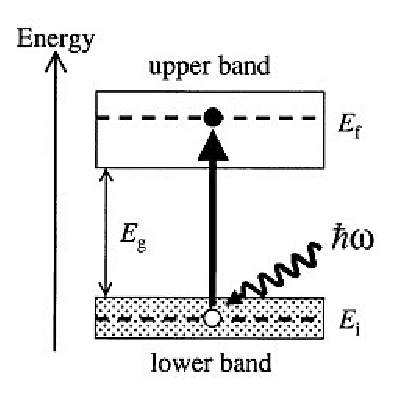
\includegraphics[width=25mm]{31.eps}
    \label{fig:3.1}
  \end{minipage}
 \\ [\intextsep]
Interband optical absorption between an initial state of energy $E_i$ in an occupied lower band and a final state at energy $E_f$ in an empty upper band. The energy difference between the two bands is $E_g$.}

Figure 3.1 shows a highly simplified energy diagram of two separated bands in a solid. The gap in energy between the bands is called the band gap Eg. Interband optical transitions will be possible between these bands if the selection rules allow them. During the transition an electron jumps from the band at lower energy to the one above it by absorbing a photon. This can only happen if there is an electron in the initial state in the lower band. Furthermore, the Pauli exclusion principle demands that the final state in the upper band must be empty. A typical example of a situation where this applies is the transitions across the fundamental band gap of a semiconductor or insulator. In this case, a photon excites an electron from the filled Yalence band to the empty conduction band.

By applying the law of conservation of energy to the interband transition shown in Fig. 3.1 we can see that:
\begin{equation}\label{equa:3.1}
  E_f=F_i+\hbar\omega
\end{equation}
where $E_i$ is the energy of the electron in the lower band, $E_f$ is the energy of the final state in the upper band, and $\hbar\omega$ is the photon energy. Since there is a continuous range of energy states within the upper and lower bands, the interband transitions will be possible over a continuous range of frequencies. The range of frequencies is determined by the upper and lower energy limits of the bands.

It is apparent from Fig. 3.1 that the minimum value of $(E_f-E_i)$ is $E_g$. This implies that the absorption shows a threshold behaviour: interband transitions will not be possible unless $\hbar\omega>E_g$. Interband transitions therefore give rise to a continuous absorption spectrum from the low energy threshold at $E_g$ to an upper value set by the extreme limits of the participating bands. This contrasts with the absorption spectrum of isolated atoms which consist of discrete lines.

The excitation of the electron leaves the initial state at energy $E_i$ in the lower band unoccupied. This is equivalent to the creation of a \textbf{hole} in the initial state. The interband absorption process therefore creates a hole in the initial state and an electron in the final state. and may be considered as the creation of an \textbf{electron-hole pair}.

In the sections that follow, we will study how the interband absorption rate depends on the band structure of the solid. At this stage we just make one general distinction based on whether the band gap is \textbf{direct} or \textbf{indirect}. This point is illustrated in Fig. 3.2. Figure 3.2(a) shows the $E-k$ diagram of a solid with a direct band gap, while Fig. 3.2(b) shows the equivalent diagram for an indirect gap material. The distinction concerns the relative positions of the conduction band minimum and the valence band maximum in the Brillouin zone. In a direct gap material, both occur at the zone centre where $k = 0$. In an indirect gap material, however, the conduction band minimum does not occur at $k = 0$, but rather at some other value of $k$ which is usually at the zone edge or close to it.

The distinction between the nature of the band gap has very important consequences for the optical properties. We will see in Section 3.2 that conservation of momentum implies that the electron wave vector does not change significantly during a photon absorption process. We therefore represent photon absorption processes by vertical lines on $E-k$ diagrams. It is immediately apparent from Fig. 3.2(b) that the electron wave vector must change significantly in jumping from the valence band to the bottom of the conduction band if the band gap is indirect. It is not possible to make this jump by absorption of a photon alone: the transition must involve a phonon to conserve momentum.This contrasts with a direct gap material in which the process may take place without any phonons being involved.

Indirect absorption plays a very significant role in technologically important materials such as silicon. The treatment of indirect absorption is more complicated than direct absorption because of the role of the phonons. We will therefore begin our discussion of interband transitions by restricting our attention to direct processes. Interband absorption processes in indirect gap materials will be considered in Section 3.4.

\section{The Transition Rate for Direct Absorption}

The optical absorption coefficient a is determined by the quantum mechanical transition rate $W_{i\rightarrow f}$ for exciting an electron in an initial quantum state $\psi_i$ to a final state $\psi_f$ by absorption of a photon of angular frequency $\omega$. Our task is therefore to calculate $W_{i\rightarrow f}$ and hence to derive the frequency dependence of $\alpha$. As discussed in Appendix B, the transition rate is given by Fermi's golden rule:
\begin{equation}\label{equa:3.2}
  W_{i\rightarrow f}=\frac{2\pi}{\hbar}|M|^2g(\hbar\omega)
\end{equation}
The transition rate thus depends on two factors:
\begin{itemize}
  \item the \textbf{matrix element} $M$,
  \item the \textbf{density of states} $g(\hbar\omega)$
\end{itemize}
In the discussion below, we consider the matrix element first, and then consider $g(\hbar\omega)$ afterwards.

The matrix element describes the effect of the external perturbation caused by the light wave on the electrons. It is given by:
\begin{eqnarray}
% \nonumber to remove numbering (before each equation)
  M &=& \langle f|H'|i\rangle \\
   &=& \int \psi_f^*(\mathrm{r})H'(\mathrm{r})\psi_i(\mathrm{r})d^3\mathrm{r}
\end{eqnarray}
where $H'$ is the perturbation associated with the light wave, and $\mathrm{r}$ is the position vector of the electron. We adopt here the semiclassical approach in which we treat the electrons quantum mechanically, but the photons are described by electromagnetic waves.

In classical electromagnetism, the presence of a perturbing electric field $\vec{\varepsilon}$ causes a shift in the energy of a charged particle equal to $-\mathrm{p}\cdot\vec{\varepsilon}$, where $\mathrm{p}$ is the dipole moment of the particle. The appropriate quantum perturbation to describe the electric dipole interaction between the light and the electron is therefore:
\begin{equation}\label{equa:3.4}
  H'=-\mathrm{p_e}\cdot\vec{\varepsilon}_{photon}
\end{equation}
where $\mathrm{P_e}$ is the electron dipole moment and is equal to $-e\mathrm{r}$. This form for the perturbation is justified more rigorously in Section B.2 of Appendix B.

The light wave is described by plane waves of the form
\begin{equation}\label{equa:3.5}
  \vec{\varepsilon}_{photon}(\mathrm{r})=\vec{\varepsilon_0}e^{\pm i \mathrm{k}\cdot\mathrm{r}}
\end{equation}
where the sign in the phase depends on the direction of propagation of the wave. The perturbation is thus:
\begin{equation}\label{equa:3.6}
  H'(\mathrm{r})=e\vec{\varepsilon_0}\cdot\mathrm{r}e^{\pm i \mathrm{k}\cdot\mathrm{r}}
\end{equation}
The electron states in a crystalline solid are described by Bloch functions. This allows us to write the wave functions as a product of a plane wave and an envelope function that has the periodicity of the crystal lattice, as discussed in Section 1.5.2 and Appendix C. We therefore write:
\begin{eqnarray}
% \nonumber to remove numbering (before each equation)
  \psi_i(\mathrm{r}) &=& \frac{1}{\sqrt{V}}u_i(\mathrm{r})e^{i\mathrm{k_i}\cdot\mathrm{r}} \\
  \psi_f(\mathrm{r}) &=& \frac{1}{\sqrt{V}}u_f(\mathrm{r})e^{i\mathrm{k_f}\cdot\mathrm{r}}
\end{eqnarray}
where $u_i$ and $u_f$ are the appropriate envelope functions for the initial and final bands respectively, and $V$ is the normalization volume. $k_i$ and $k_f$ are the wave vectors of the initial and final electron states.

On substituting the perturbation of eqn 3.6 and the wave functions of eqns 3.7 and 3.8 into eqn 3.3, we obtain:
\begin{equation}\label{equa:3.9}
  M=\frac{e}{V}\int u_f^*{\mathrm{r}}e^{-i\mathrm{k_f}\cdot\mathrm{r}}(\vec{\varepsilon_0}\cdot\mathrm{r}e^{\pm i\mathrm{k}\cdot\mathrm{r}})u_i(\mathrm{r})e^{i\mathrm{k_i}\cdot\mathrm{r}}d^3\mathrm{r}
\end{equation}
where the limits of the integration are over the whole crystal. This integral can be simplified by invoking conservation of momentum and Bloch's theorem. Conservation of momentum demands that the change in crystal momentum of the electron must equal the momentum of the photon, that is:
\begin{equation}\label{equa:3.10}
  \hbar\mathrm{k_f}-\hbar\mathrm{k_i}=\pm\hbar\mathrm{k}
\end{equation}
This is equivalent to requiring that the phase factor in eqn 3.9 must be zero. If the phase factor is not zero, the different unit cells within the crystal will be out of phase with each other and the integral will sum to zero. Bloch's theorem requires that Ui and Uf are periodic functions with the same periodicity as the lattice.

These two considerations imply that we can separate the integral over the whole crystal into a sum over identical unit cells, because the unit cells are equivalent and in phase. We thus obtain:
\begin{equation}\label{equa:3.11}
  |M|\approx\int_{unit cell}u_i^*(\mathrm{r})xu_f(\mathrm{r})d^3\mathrm{r}
\end{equation}
where we have defined our axes in such a way that the light is polarized along the $x$ axis. This matrix element represents the electric dipole moment of the transition. Its evaluation requires knowledge of the envelope functions $u_i$ and $u_f$. These functions are derived from the atomic orbitals of the constituent atoms, and so each material has to be considered separately.

The conservation of momentum condition embodied in eqn 3.10 can be simplified further by considering the magnitude of the wave vectors of the electrons and photons. The wave vector of the photon is $2\pi/\lambda$, where $\lambda$ is the wavelength of the light. Optical frequency photons therefore have $k$ values of about $10^7 m^{-1}$. The wave vectors of the electrons, however, are much larger. This is because the electron wave vector is related to the size of the Brillouin zone, which is equal to $\pi/a$, where $a$ is the unit cell dimension. Since $a\sim 10^{-10} m$, the photon wave vector is much smaller than the size of a Brillouin zone. Therefore we may neglect the photon momentum in eqn 3.10 in comparison to the electron momentum and write:
\begin{equation}\label{3.12}
  \mathrm{k_f}=\mathrm{k_i}
\end{equation}
A direct optical transition therefore leads to a negligible change in the wave vector of the electron. This is why we represent the absorption processes by vertical arrows in the electron $E-k$ diagrams such as the ones shown in Fig. 3.2.

The $g(\hbar\omega)$ factor that appears in eqn 3.2 is the \textbf{joint density of states} evaluated at the photon energy. As explained in Section 1.5.4, the density of states function describes the distribution of the states within the bands. The \textit{joint} density of states accounts for the fact that both the initial and final electron states lie within continuous bands. For electrons within a band, the density of states per unit energy range $g(E)$ is obtained from:
\begin{equation}\label{equa:3.13}
  g(E)dE=2g(k)dk
\end{equation}
where $g(k)$ is the density of states in momentum space. The extra factor of 2 here compared to eqn 1.29 allows for the fact that there are two electron spin states for each allowed $k$-state. This gives:
\begin{equation}\label{equa:3.14}
  g(E)=\frac{2g(k)}{dE/dk}
\end{equation}
where $dE/dk$ is the gradient of the $E-k$ dispersion curve in the band diagram. $g(k)$ itself is worked out by calculating the number of $k$-states in the incremental volume between shells in $k$-space of radius $k$ and $k + dk$. This is equal to the number of states per unit volume of $k$-space, namely $1/(2\pi)^3$ (see Exercise 3.1), multiplied by the incremental volume $4\pi k^2dk$. Hence $g(k)$ is given by the standard formula:
\begin{eqnarray}\label{equa:3.15}
% \nonumber to remove numbering (before each equation)
  g(k)dk &=& \frac{1}{(2\pi)^3}4\pi k^2dk \\
  \Rightarrow g(k) &=& \frac{k^2}{2\pi^2}
\end{eqnarray}
We can then work out $g(E)$ by using eqn 3.14 if we know the relationship between $E$ and $k$ from the band structure of the material. For electrons in a parabolic band with effective mass $m^*$. $g(E)$ is given by (see Exercise 3.2):
\begin{equation}\label{equa:3.16}
  g(E)=\frac{1}{2\pi^2}(\frac{2m*}{\hbar^2})^{\frac{3}{2}}E^{\frac{1}{2}}
\end{equation}
This is just the standard formula for free electrons but with the free electron mass $m_0$ replaced by  $m^*$.

The joint density of states factor is finally obtained by evaluating $g(E)$ at $E_i$ and $E_f$ when they are related to $\hbar\omega$ through the details of the band structure. We will see how to do this in the case of parabolic bands in Section 3.3.3. The density of atoms in a solid is very large, and so the density of states factor will be high and the transition rate correspondingly large. It is common to find values of $\alpha$ in the range $10^6-10^8 m^{-1}$ for the direct absorption coefficient in a solid.

The results derived here are of general applicability for interband transitions in crystalline solids. To proceed further, we need detailed knowledge of the band structure. In the next section we will use these general results to derive the frequency dependence of the absorption near the band edge of a direct gap semiconductor.

\section{Band Edge Absorption in Direct Gap Semiconductors}
The basic process for an optical transition across the fundamental band gap of a direct gap semiconductor is shown in Fig. 3.2(a). An electron is excited from the valence band to the conduction band by absorption of a photon. The transition rate is evaluated by working out the matrix element and the density of states, as discussed in the preceding section. These factors are considered separately below.

\subsection{The atomic physics of the interband transitions}
The matrix element that we need to evaluate is given in eqn 3.11. This allows us to calculate the probability for electric dipole transitions if we know the atomic character of the envelope wave functions $u_i(\mathrm{r})$ and $u_f(\mathrm{r})$. The full treatment of this problem employs group theory to determine the character of the bands involved. This approach is beyond the scope of our present discussion, and at this level we will just offer a few intuitive arguments.

The semiconductors that we will be considering all have four valence electrons. This is obvious in the case of the elemental semiconductors such as silicon and germanium, which come from group IV of the periodic table. It is also true, however, for the binary compounds made from elements symmetrically displaced from group IV of the periodic table. The covalent bond in these compounds is made by sharing the electrons in such a way that each atom ends up with four electrons. For example, the bond in the III-V compounds is formed by sharing the five valence electrons from the group V element with the three from the group III element, giving a total of eight electrons for every two atoms. It is energetically favourable to do this because it is then possible to form very stable covalent crystals with a structure similar to diamond. Similar arguments apply to the II-VI semiconductor compounds.

The valence electrons of a four-valent atom are derived from the $s$ and $p$ orbitals. For example, the electronic configuration of germanium is $4s^24p^2$. In the crystalline phase the adjacent atoms share the valence electrons with each other in a covalent bond. Figure 3.3 shows schematically the evolution of the $s$ and $p$-like atomic states, through the $s$ and $p$ bonding and antibonding orbitals of the molecule, to the valence and conduction bands of the crystalline solid. The level ordering shown is appropriate for most III-V and II-VI semiconductors, as well as germanium. The level ordering in silicon is different: see Exercise 3.9.

The evolution of the levels shown in Fig. 3.3 makes it apparent that the top of the valence band has a $p$-like atomic character, while the bottom of the conduction band is $s$-like. This is because the four valence electrons occupy the four bonding orbitals, which then evolve into the valence band. The top of the valence band is derived from the $p$ bonding orbitals, while the bottom of the conduction band originates from the $s$ antibonding orbitals. Therefore optical transitions from the valence band to the conduction band are from $p$-like states to $s$-like states. We know from the selections rules for dipole transitions that $p \rightarrow s$ transitions are allowed. (See Exercise 3.3 and Section B.3 in Appendix B.) Hence we conclude that the transitions between the valence band and the conduction band of a semiconductor with a level ordering such as the one shown in Fig. 3.3 are electric-dipole allowed.

The conclusion of this discussion is that the probability for interband transitions across the band gap in materials like germanium or the III-V compounds is high, and we therefore expect to observe strong absorption. This is indeed the case, as we will see below. The discussion of germanium is complicated because it has an indirect band gap. We will therefore concentrate our attention on the III-V compound semiconductor gallium arsenide. GaAs has a direct band gap, and the level ordering follows the scheme shown in Fig. 3.3. The transitions across the gap are therefore both dipole-allowed and direct. This makes GaAs a standard example for considering direct interband transitions. It is also a very important material for optoelectronic applications.

\subsection{The band structure of a direct gap 111-V semiconductor}

The band structure of GaAs in the energy range near the fundamental band gap is shown in Fig. 3.4. The energy $E$ of the electrons in the different bands is plotted against the electron wave vector $\mathrm{k}$. GaAs has the zinc-blende structure, which is based on the face-centred cubic (f.c.c.) lattice. The band dispersion is shown for increasing $\mathrm{k}$ along two different directions of the Brillouin zone. The right hand side of the figure corresponds to moving from the zone centre where $\mathrm{k}=(0, 0, 0)$ along the (100) direction to the zone edge at $\mathrm{k} = \frac{2\pi}{a} (1, 0, 0)$, $a$ being the length of the cube edge in the f.c.c. lattice. The left hand side corresponds to moving from $\mathrm{k}=0$ along the body diagonal direction until reaching the zone edge at $\mathrm{k} = \frac{\pi}{a}(1 , 1, 1)$.

The figure is divided into a shaded region and an unshaded region. The shading represents the occupancy of the levels in the bands: bands that fall in the shaded region are below the Fermi level and are full of electrons. The three bands in the shaded region therefore correspond to valence band states. The single band above the shaded region is empty of electrons and is therefore the conduction band. The three bands in the valence band correspond to the three $p$ bonding orbitals shown in Fig. 3.3, while the single conduction band corresponds to the $s$ antibonding state. This correspondence between the bands and the molecular orbitals is strictly valid only at the $\Gamma$ point at the Brillouin zone centre. The atomic character (or more accurately, the symmetry) of the bands actually changes as k increases, and is only well defined at high symmetry points in the Brillouin zone such as $\Gamma$, $X$ or $L$.

\marginnote{
\begin{minipage}{\textwidth}
    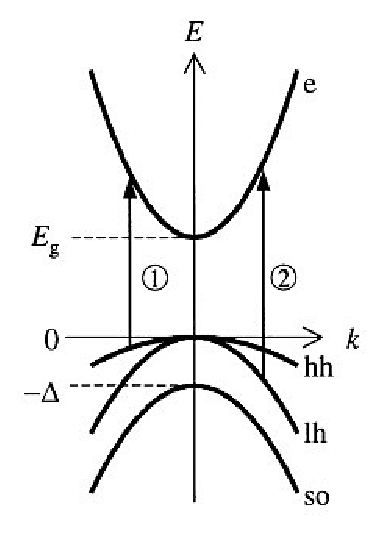
\includegraphics[width=25mm]{35.eps}
    \label{fig:3.5}
  \end{minipage}
 \\ [\intextsep]
Band structure of a direct gap III-V semiconductor such as GaAs near $k = 0$. $E = 0$ corresponds to the top of the valence band. while $E = E_g$ corresponds to the bottom of the conduction band. Four bands are shown: the heavy hole (hh) band, the light hole (lh) band, the split-off hole (so) band, and the electron ( e) band. Two optical transitions are indicated. Transition 1 is a heavy hole transition, while transition 2 is a light hole transition. Transitions can also take place between the split-off hole band and the conduction band, but these are not shown for the sake of clarity. This four-band model was originally developed for InSb in reference [2].}

In this section we are interested in the transitions that take place across the band gap for small $k$ values close to the $\Gamma$ point. This means that the correspondence to Fig. 3.3 will be justified in our discussion here. We can therefore assume that the transitions are dipole-allowed, and concentrate on working out the density of states for the transition. To do this, it is helpful to make use of the simplified four-band model shown in Fig. 3.5. This model band diagram is typical of direct gap III-V semiconductors near $k = 0$. There is a single $s$-like conduction band and three $p$-like valence bands. All four bands have parabolic dispersions. The positive curvature of the conduction band on the $E-k$ diagram indicates that it corresponds to an electron (e) band, while the negative curvature of the valence bands correspond to hole states. Two of the hole bands are degenerate at $k = 0$. These are known as the heavy (hh) and light hole (lh) bands, the heavy hole band being the one with the smaller curvature. The third band is split-off to lower energy by the spin-orbit coupling, and is known as the split-off (so) hole band. The energy difference between the maximum of the valence band and the minimum of the conduction band is the band gap $E_g$, while the spin-orbit splitting between the hole bands at $k = 0$ is usually given the symbol $\Delta$.

The schematic diagram of Fig. 3.5 should be compared with the detailed band structure of GaAs shown previously in Fig. 3.4. The maxima of the valence band occur at the $\Gamma$-point of the Brillouin zone, while the conduction band has a \lq camel back\rq structure, with minima at the $\Gamma$-point, the $L$-point and near the $X$-point. We can neglect the subsidiary minima at the $L$-point and near the $X$-point here because momentum conservation does not allow direct transitions to these states from the top of the valence band. The bands near the zone centre are all approximately parabolic, and so the simplified picture in Fig. 3.5 is valid near $k = 0$.

The three valence band states all have $p$-like atomic character, and so it is possible to have electric dipole transitions from each of the bands to the conduction band. Two such transitions are indicated on Fig. 3.5. As noted earlier, these absorption processes are represented by vertical arrows on the $E-k$ diagram. This means that the $k$ vector of the electron and hole created by the transition are the same (cf. eqn 3.12). The transition labelled 1 involves the excitation of an electron from the heavy hole band to the electron band. Transition 2 is the corresponding process originating in the light hole band. Direct transitions are also possible from the split-off band to the conduction band, but these are not shown in the figure for clarity.

\subsection{The joint density of states}

The frequency dependence of the absorption coefficient can now be calculated if we know the joint density of states factor given in eqn 3.14. This can be calculated analytically for the simplified band structure shown in Fig. 3.5.

The dispersion of the bands is determined by their respective effective masses, namely $m_e^*$ for the electrons, $m_{hh}^*$ for the heavy holes, $m_{lh}^*$ for the light holes, and $m_{so}^*$ for the split-off holes. This allows us to write the following $E-k$ relationships for the conduction, heavy hole, light hole, and split-off hole bands respectively:
\begin{eqnarray}
% \nonumber to remove numbering (before each equation)
  E_c(k) &=& E_g+\frac{\hbar^2k^2}{2m_e^*} \\
  E_{hh}(k) &=& -\frac{\hbar^2k^2}{2m_{hh}^*} \\
  E_{lh}(k) &=& -\frac{\hbar^2k^2}{2m_{lh}^*} \\
  E_{so}(k) &=& -\Delta-\frac{\hbar^2k^2}{2m_{so}^2}
\end{eqnarray}
It is evident from Fig. 3.5, that conservation of energy during a heavy hole or light hole transition requires that:
\begin{equation}\label{equa:3.21}
  \hbar\omega=E_g+\frac{\hbar^2k^2}{2m_e^*}+\frac{\hbar^2k^2}{2m_h^*}
\end{equation}
where $m_h^* = m_{hh}^*$ or $m_{lh}^*$ for the heavy or light hole transition respectively. We define the reduced electron-hole mass $\mu$ according to:
\begin{equation}\label{equa:3.22}
  \frac{1}{\mu}=\frac{1}{m_e^*}+\frac{1}{m_h^*}
\end{equation}
This allows us to rewrite eqn 3.21 in the simpler form:
\begin{equation}\label{equa:3.23}
  \hbar\omega=E_g+\frac{\hbar^2k^2}{2\mu}
\end{equation}
We are interested in evaluating $g(E)$ with $E = \hbar\omega$. The joint electron-hole density of states can be worked out by substituting eqn 3.23 into eqns 3.14 and 3.15. This gives:
\begin{eqnarray}
% \nonumber to remove numbering (before each equation)
  \text{For}\quad\hbar\omega<E_g,g(\hbar\omega) &=& 0 \\
  \text{For}\quad\hbar\omega\ge E_g,g(\hbar\omega)&=&\frac{1}{2\pi^2}(\frac{2\mu}{\hbar^2})^{\frac{3}{2}}(\hbar\omega-E_g)^{\frac{1}{2}}
\end{eqnarray}
We therefore see that the density of states factor rises as $(\hbar\omega-E_g)^{\frac{1}{2}}$ for photon energies greater than the band gap.

\subsection{The frequency dependence of the band edge absorption}
Now that we have discussed the matrix element and the density of states, we can put it all together and deduce the frequency dependence of the absorption coefficient $\alpha$. Fermi's golden rule given in eqn 3.2 tells us that the absorption rate for a dipole-allowed interband transition is proportional to the joint density of states given by eqn 3.24. We therefore expect the following behaviour for $\alpha(\hbar\omega)$:
\begin{eqnarray}
% \nonumber to remove numbering (before each equation)
 \text{For}\quad \hbar\omega<E_g,\alpha(\hbar\omega) &=& 0 \\
 \text{For}\quad \hbar\omega\ge E_g,\alpha(\hbar\omega)&\approx& (\hbar\omega-E_g)^{\frac{1}{2}}
\end{eqnarray}
There is no absorption if $\hbar\omega< E_g$, and the absorption increases as $(\hbar\omega-E_g)^{1/2}$ for photon energies greater than the band gap. We also expect that transitions with larger reduced masses will give rise to stronger absorption due to the $\mu^{\frac{3}{2}}$ factor in eqn 3.24.

The predictions of eqn 3.25 can be compared to experimental data. Figure 3.6 shows results for the absorption coefficient of the direct gap III-V semiconductor indium arsenide at room temperature. The graph plots $\alpha^2$ against the photon energy in the spectral region close to the band gap. The straight line relationship between $\alpha^2$ and ($\hbar\omega-E_g$) indicates that the model we have developed is a good one. The band gap can be read from the data as the point at which the absorption goes to zero. This gives a value of 0.35 eV, which is in good agreement with values deduced from electrical measurements. Note that the values of the absorption coefficient are very large. This is a consequence of the very large density of states in the solid phase.

In many III-V semiconductors, including GaAs itself, it is found that the frequency dependence predicted by eqn 3.25 is only approximately obeyed. There are a number of reasons for this.
\begin{itemize}
  \item We have neglected the Coulomb attraction between the electron and hole, which can enhance the absorption rate and cause exciton formation. These effects become stronger as the band gap gets larger and the temperature is lowered. This is why we have presented room temperature data for a semiconductor with a smallish band gap in Fig. 3.6. Excitonic effects are very significant in materials like GaAs even at room temperature. This point will be discussed further in Chapter 4, and is clearly apparent in the absorption data for GaAs shown in Fig. 4.3.
  \item The semiconductor may contain impurity or defect states with energies within the band gap, and these may allow absorption for photon energies less than the band gap. This point is discussed in Section 7.4.2.
  \item The parabolic band approximations embodied in the dispersion relations of eqns 3.17-3.20 is only valid near $k = 0$. As the photon energy increases above the band gap, the joint density of states will no longer obey the frequency dependence given in eqn 3.24. In these cases we must use the full band structure to evaluate the density of states. We  will give a discussion of how this is done in Section 3.5 below.
\end{itemize}

\subsection{The Franz-Keldysh effect}

The modification of the band edge absorption by the application of an external electric field $\vec{\varepsilon}$ was studied independently by W. Franz and L.V. Keldysh in 1958. They showed that there are two main effects:
\begin{itemize}
  \item The absorption coefficient for photon energies less than $E_g$ is no longer zero, as stated in eqn 3.25, but now decreases exponentially with ($E_g - \hbar\omega$). The frequency dependence of $\alpha$ is given by:
      \begin{equation}\label{equa:3.26}
        \alpha(\hbar\omega)\approx\exp\left(-\frac{4\sqrt{2m_e^*}}{3|e|\hbar\varepsilon}(E_g-\hbar\omega)^{3/2}\right)
      \end{equation}
      This implies that the band edge shifts to lower energy as the field is increased. (See Exercise 3.11.)
  \item The absorption coefficient for $\hbar\omega>E_g$ is modulated by an oscillatory function. The oscillations in $\alpha(\hbar\omega)$ are called Franz-Keldysh oscillations.
\end{itemize}

These two effects are collectively known as the \textbf{Franz-Keldysh effect}. They are typically observed when the semiconductor is incorporated as a thin i-region at the junction of a p-n diode. This allows controllable fields to be applied by varying the bias on the device, as explained in Appendix D.

It can be seen from the Kramers-Kronig relationship given in eqn 2.36 that a change in the absorption coefficient will produce changes in the refractive index at frequencies below the band gap. Thus the application of the electric field modulates both the absorption and the refractive index of the material. This modulation of the optical constants by the electric field is an example of an \textbf{electro-optic effect}. The changes may be either linear or quadratic in the field. In Sections 11.3.1 and 11.4.1 of Chapter 11, we will explain how  these effects ~an be described in terms of nonlinear optical susceptibility tensors.

The changes in the real and imaginary parts of the refractive index produced by the electric field imply that the reflectivity will also be changed through eqn 1.26. This is the basis of the technique of \textbf{electroreflectance}, in which the modulation of the reflectivity in response to an AC electric field is measured as a function of the photon energy. The electroreflectance technique is widely used to determine important band structure parameters.

\subsection{Band edge absorption in a magnetic field}
It is well known in classical physics that the application of a strong magnetic field with flux density $B$ causes electrons to perform circular motion around the field at the \textbf{cyclotron frequency} $\omega_c$ given by (see Exercise 3.12):
\begin{equation}\label{equa:3.27}
  \omega_c=\frac{eB}{m_0}
\end{equation}
In classical physics, the radius of the orbit and the energy can have any values, but in quantum physics, they are both quantized. The quantized energies are given by:
\begin{equation}\label{equa:3.28}
  E_{\texttt{n}}=(\texttt{n}+\frac{1}{2})\hbar\omega_c
\end{equation}
where $\texttt{n} = 0, 1, 2, \cdots$ These quantized energy levels are called \textbf{Landau levels}.

Consider a semiconductor in the presence of a strong magnetic field along the $z$ direction. The motion of the electrons in the conduction band and holes in the valence band will be quantized in the $x$, $y$ plane, but their motion will still be free in the $z$ direction. Their energies within the bands will thus be given by:
\begin{equation}\label{equa:3.29}
  E^{\texttt{n}}(k_z)=(n+\frac{1}{2})\frac{e\hbar B}{m^*}+\frac{\hbar^2k_z^2}{2m*}
\end{equation}
where $m^*$ is the appropriate effective mass. The first term gives the energy of the quantized motion in the $(x, y)$ plane, while the second describes the free motion along the $z$ direction. In absolute terms relative to $E = 0$ at the top of the valence band, the electron and hole energies are given by:
\begin{eqnarray}
% \nonumber to remove numbering (before each equation)
\nonumber  E_{\texttt{n}}^e(k_z) &=& E_g+(\texttt{n}+\frac{1}{2})\frac{e\hbar B}{m_e^*}+\frac{\hbar^2k_z^2}{2m_e^*}  \label{equa:3.30}\\
  E_{\texttt{n}}^h(k_z) &=& -(\texttt{n}+\frac{1}{2})\frac{e\hbar B}{m_h^*}-\frac{\hbar^2k_z^2}{2m_h^*} \label{equa:3.31}
\end{eqnarray}
These are equivalent to eqns \ref{equa:3.17}, \ref{equa:3.18} and \ref{equa:3.19}, which are valid at $B = 0$.

If the sample is illuminated when the field is applied, an interband transition can take place in which an electron is created in the conduction band and a hole is created in the valence band. It can be shown that the Landau level number n does not change during the interband transition. (See Exercise 3.12.) This selection rule implies that the electron and hole must have the same value of $\texttt{n}$. Furthermore, the $k_z$ value of both particles must be the same because the photon has negligible momentum. Therefore, the transition energy will be given by:
\begin{eqnarray}
% \nonumber to remove numbering (before each equation)
\nonumber  \hbar\omega &=& E_{\texttt{n}}^e(k_z)-E_{\texttt{n}}^h(k_z) \\
   &=& E_g+(\texttt{n}+\frac{1}{2})\frac{e\hbar B}{\mu}+\frac{\hbar^2k_z^2}{2\mu} \label{equa:3.32}
\end{eqnarray}
where $\mu$ is the reduced mass given in eqn 3.22. Equation 3.31 should be compared to eqn 3.23 which applies when $B = 0$. The term in $k_z$ is unchanged, but the $x$ and $y$ components of $\mathrm{k}$ are now quantized by the magnetic field. The frequency dependence of the absorption coefficient which follows from eqn 3.31 is considered in detail in Exercise 3.13. In brief, we expect very high absorption at any photon energy that can satisfy eqn 3.31 with $k_z=0$. This gives rise to a series of equally spaced peaks in the absorption spectrum with energies given by
\begin{equation}\label{equa:3.32}
  \hbar\omega=E_g+(\texttt{n}+\frac{1}{2})\frac{e\hbar B}{\mu};\qquad \texttt{n}=0,1,2,\cdots
\end{equation}
One immediate consequence of this result is that we expect the absorption edge to shift to higher energy by $\hbar eB/2\mu$ in the magnetic field.

Figure 3.7 shows the room temperature transmission spectrum of germanium at $B = 0$ and $B = 3.6 T$. We see that at $B = 3.6 T$ the absorption edge is indeed shifted to higher energy and there is a regularly spaced series of dips in the transmission, as predicted by eqn 3.32. The spectral width of the dips is determined mainly by line broadening due to scattering. The electron effective mass can be determined from the energies of the minima in the transmission: see Exercise 3 .13.

\section{Band Edge Absorption in Indirect Gap Semiconductors}

In the previous two sections, we have been concentrating on direct interband transitions. As it happens, several of the most important semiconductors have indirect band gaps, most notably: silicon and germanium. Indirect gap semiconductors have their conduction band minimum away from the Brillouin zone centre, as shown schematically in Fig. 3.2(b). Transitions at the band edge must therefore involve a large change in the electron wave vector. Optical frequency photons only have a very small $k$ vector, and it is not possible to make this transition by absorption of a photon alone: the transition must involve a phonon to conserve momentum.

Consider an indirect transition that excites an electron in the valence band in state $(E_i, \mathrm{k_i})$ to a state $(E_f, \mathrm{k_f})$ in the conduction band. The photon energy is $\hbar\omega$, while the phonon involved has energy $\hbar\Omega$ and wave vector $\mathrm{q}$. Conservation of energy demands that:
\begin{equation}\label{equa:3.33}
  E_f=E_i+\hbar\omega\pm\hbar\Omega
\end{equation}
while conservation of momentum requires that:
\begin{equation}\label{equa:3.34}
  \hbar\mathrm{k_f}=\hbar\mathrm{k_i}\pm\hbar\mathrm{q}
\end{equation}
The $\pm$ factors allow for the possibility of phonon absorption or emission, with the $+$ sign corresponding to absorption, and the $-$ sign to emission. We have neglected the photon's momentum in eqn 3.34. This approximation was justified previously in connection with eqn 3.12.

Before considering the shape of the band edge absorption spectrum, we can first make a general point. Indirect transitions involve both photons and phonons. In quantum mechanical terms, this is a second-order process: a photon must be destroyed, and a phonon must be either created or destroyed. This contrasts with direct transitions which are first-order processes because no phonons are involved. The transition rate for indirect absorption is therefore much smaller than for direct absorption.

The smaller transition rate for indirect processes is clearly shown by the data given in Fig. 3.8, which compares the band edge absorption of silicon and GaAs. Silicon has an indirect band gap at 1.12 eV, while GaAs has a direct gap at 1.42eV. We see that the absorption rises much faster with frequency in the direct gap material, and soon exceeds the indirect material even though its band gap is larger. The absorption of GaAs is roughly an order of magnitude larger than that of silicon for energies greater than $\sim 1.43\mathrm{eV}$.

The derivation of the quantum mechanical transition rate for an indirect gap semiconductor is beyond the scope of this book. The results of such a calculation give the following result:
\begin{equation}\label{equa:3.35}
  \alpha^{indirect}(\hbar\omega)\approx(\hbar\omega-E_g\mp\hbar\Omega)^2
\end{equation}
This shows that we expect the absorption to have a threshold close to $E_g$, but not exactly at $E_g$. The difference is $\mp\hbar\Omega$, depending on whether the phonon is absorbed or emitted. Note that the frequency dependence is different to that for direct gap semiconductors given in eqn 3.25. This provides a convenient way to determine whether the band gap is direct or not. Furthermore, the involvement of the phonons gives other tell-tale signs that the band gap is indirect, as we will discuss below.

Indirect absorption has been thoroughly studied in materials like germanium. The band structure of germanium is shown in Fig. 3.9. The overall shape of the band dispersion is fairly similar to that of GaAs given in Fig. 3.4. There is, however, one very important qualitative difference: the lowest conduction band minimum of germanium occurs at the $L$ point, where $k =\frac{\pi}{a}(1,1,1)$, and not at $k = 0$. This makes germanium an indirect gap semiconductor. The value of the indirect gap is 0.66eV, which corresponds to the band gap determined by electrical measurements. This is 0.14eV smaller than the direct gap at $k = 0$.

Figure 3.10 shows the results of absorption measurements on germanium at room temperature. $\sqrt{\alpha}$ is plotted against $\hbar\omega$ in the spectral region close to the band gap at 0.66 eV. The data fits well to a straight line, which confirms the prediction of eqn 3.35. The data extrapolates back to 0.65 eV, which indicates from eqn 3.35 that a phonon of energy $\sim$0.01 eV has been absorbed. The wave vector $\mathrm{q}$ of the phonon must be equal to that of an electron at the $L$-point of the Brillouin zone. The energies of the four different phonon modes with the required wave vector are listed in Table 3.1, from where we see that it must be TA phonons that are involved. The experimental data also shows a tail extending down to about 0.60 eV. This is caused by absorption of the higher frequency phonons and also multiphonon absorption.

The probability for phonon absorption is proportional to the number of phonons present, which is given by the Bose-Einstein formula:
\begin{equation}\label{equa:3.36}
  f_{BE}(E)=\frac{1}{\exp(E/k_BT)-1}
\end{equation}
The variation of the phonon populations with temperature implied by eqn 3.36 leads to a characteristic temperature dependence of the absorption edge. As we decrease $T$, the contributions due to phonon absorption gradually freeze out, starting with the highest energy phonons. At very low temperatures, we would not expect to observe any phonon absorption at all, because there would be no phonons excited with enough energy. On the other hand, phonon emission is possible at all temperatures. Thus at the lowest temperatures, the indirect absorption edge would be determined by phonon emission rather than phonon absorption. This behaviour contrasts with direct gap materials, in which the absorption edge merely shifts with the band gap as the temperature is varied.

The band diagram for germanium in Fig. 3.9 shows that direct transitions can occur if the photon energy exceeds 0.80 eV. In this case, we would expect that the absorption would begin to follow eqn 3.25 instead of eqn 3.35. This is indeed borne out by the data. The black squares in Fig. 3.10 show the absorption data on a new scale, with $\alpha^2$ plotted against the photon energy. A clear threshold at 0.80 eV is observed, and the frequency dependence approximately obeys $\alpha^2\approx(\hbar\omega-E_g^{dir})$, where $E_g^{dir}=0.80$ eV is the band gap for direct transitions at the $\Gamma$ point. Note that the direct absorption completely dominates over the indirect processes once we have crossed the second threshold at $E_g^{dir}$. The indirect absorption is much weaker, and is insignificant when plotted on the same scale as the direct absorption as in Fig. 3.10. This highlights the second-order nature of the indirect absorption.

\section{Interband Absorption above the Band Edge}

Up to this point, we have been concentrating on the absorption near the band edge. As we will see in Chapter 5, the reason for doing this is that the optical properties at the band edge determine the emission spectra. This does not mean that the rest of the absorption spectrum is uninteresting: it is just more complicated to deal with because the parabolic band approximation does not apply. However, as we will see below, much useful information about the full band structure can be obtained from analysis of the overall spectrum.

It is not possible to give explicit formulae for the full frequency dependence of the absorption spectrum as we did for the band edge absorption in eqns 3.25 and 3.35. Instead, we have to work out $dE/dk$ in eqn 3.14 from the full band structure. In this section we will illustrate how this is done for the case of silicon. The principles described here can be applied to other materials if the band structure is known.

Figure 3 .11 shows the interband absorption spectrum of silicon up to 10 eV. Two features at about 3.5 eV and 4.3 eV are readily identified in the data. These two energies are labelled $E_1$ and $E_2$ and are related to aspects of the band structure, as discussed further below. The absorption coefficient in the spectral region around $E_1$ and $E_2$ is extremely large, with values of $\alpha$ in excess of $10^8 m^{-1}$. This should be compared to values of $10^2-10^6 m^{-1}$ in the spectral region immediately above the band gap $E_g$ at 1.1 eV. (See Fig. 3.8.) Indeed, the band edge absorption is completely negligible on the scale of the data shown in Fig. 3.11. This is a consequence of two factors. Firstly, the band edge absorption is weak because it is indirect, and secondly, the density of states at the band edge is comparatively small. The measured absorption spectrum is actually dominated by direct absorption at photon energies where the density
of states is very high.

Figure 3.12 shows the band structure of silicon along the $(100)$ and $(111)$ directions. The band gap $E_g$ is indirect and has a value of 1.1 eV, with the conduction band minimum located near the $X$-point of the Brillouin zone. Direct transitions can take place between any state in the valence band and the conduction band states directly above it, if the transitions are dipole-allowed. The minimum direct separation between the conduction and valence bands occurs near the $L$ point, where the transition energy is 3.5 eV. The energy of these transitions is labelled $E_1$, and corresponds to the sharp increase in the absorption at 3.5 eV observed in the data shown in Fig. 3.11. The separation of the conduction and valence bands near the $X$ point is also significant. This energy is labelled $E_2$ and corresponds to the absorption maximum at 4.3 eV.

The transitions near the $L$ and $X$ points are particularly important because of the \lq camel's back\rq shape of the conduction band. This means that the conduction band ends up having a negative curvature near these points of the Brillouin zone. The curvature is more or less the same as that in the valence band, so that the conduction and valence bands are approximately parallel to each other. This means that we can have direct transitions with the same photon energy for many different values of $k$. The joint density of states factor is therefore very high at $E_1$ and $E_2$, and we expect the absorption to be correspondingly high. This is indeed observed in the experimental data: the absorption rises sharply at $E_1$ and reaches a peak at $E_2$. The absolute values of the absorption coefficient are extremely large: over $10^8 m^{-1}$ as we have already noted.

\marginnote{
\begin{minipage}{\textwidth}
    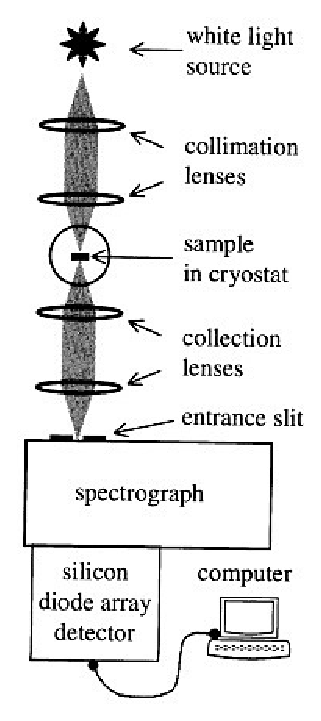
\includegraphics[width=25mm]{313.eps}
    \label{fig:3.13}
  \end{minipage}
 \\ [\intextsep]
Schematic diagram of an experimental arrangement to measure absorption spectra in the wavelength range 200- 1000 nm using a silicon diode array detector. At longer wavelengths the spectrograph and silicon detector is replaced with a scanning monochromator and an infrared detector, or with a Fourier transform spectrometer.}

In a region of the Brillouin zone where the bands are parallel, the photon energy $E$ for direct transitions does not depend on $k$. This implies that $dE/dk$ is zero, and hence that the joint density of states $g(E)$ diverges (cf. eqn 3.14). The energies at which $dE /dk$ vanishes are called \textbf{critical points}, and the corresponding divergences in the density of states are called \textbf{Van Hove singularities}. In practice, the bands are only approximately parallel over a portion of the Brillouin zone, and so $g(\hbar\omega)$ just become very large, rather than diverging completely.

The discussion of the absorption coefficient of silicon given here can be adapted to other materials if their band structure is known. The absorption strength will be proportional to the joint density of states, which will be particularly high if the conduction and valence bands are parallel to each other. An example of how this is done in the case of metals is discussed in Section 7.3.2 of Chapter 7.

\section{Measurement of Absorption Spectra}

The absorption coefficient of a material is usually determined by measuring the transmission of a thin platelet sample. A typical experimental arrangement to do this is shown in Fig. 3.13. The light from a low intensity white light source such as a tungsten bulb is passed through the sample, and the spectrum of the transmitted light is recorded with a spectrograph and a silicon diode array detector. The transmission coefficient is determined by calculating the ratio of the light on the detector with and without the sample present. The absorption coefficient is then calculated from the transmission using eqn 1.6, after measuring the reftectivities in a separate experiment. By placing the sample in a helium cryostat, the absorption coefficient can be measured as a function of temperature down to 2 K.

The arrangement shown in Fig. 3.13 can be used for measurements within the spectral response of silicon, namely  $\sim200-1000 \mathrm{nm}$. At longer wavelengths the spectrograph and silicon detector must be replaced by a scanning monochromator with a suitable infrared detector. The criteria used to select the optimal detector for a particular spectral region are discussed in Section 3.7.1. At wavelengths beyond $\sim5\mu m$, it is common to use Fourier transform spectrometers for absorption measurements.

In some materials, the absorption is so strong that it is impractical to use transmission measurements to determine $\alpha$. We have already seen, for example, that the absorption coefficient of silicon exceeds $10^8 m^{-1}$ at some wavelengths, which would mean that the transmission of a very thin sample of thickness $0.1\mu m$ would still be less than $0.01\%$. In this case, the absorption is calculated from the imaginary part of the complex refractive index using eqn 1.16. $\kappa$ itself is deduced from the measured reflectivity spectra $R(\hbar\omega)$ using eqn 1.26. This might seem impossible at first sight, because $R$ depends on both $n$ and $\kappa$. However, we know from Section 2.2.5 that $n$ and $\kappa$ are not completely independent variables and must be related to each other through the Kramers-Kronig relationships. Hence by self-consistent fitting of the reflectivity spectra using the Kramers-Kronig formulre given in eqns 2.36 and 2.37, we can determine both $n$ and $\kappa$ from $R(\hbar\omega)$, and hence deduce $\alpha$ from $\kappa$.

\section{Semiconductor Photodetectors}

The strong absorption found in semiconductors is the basis of semiconductor \textbf{photodetectors}. Light with photon energy greater than the band gap is absorbed in the semiconductor, and this creates free electrons in the conduction band and free holes in the valence band. The presence of the light can therefore be detected either by measuring a change in the resistance of the sample or by measuring an electrical current in an external circuit. In this section we consider the operating principles of two different types of detector, and then discuss the use of semiconductor detectors in solar cells.

\subsection{Photodiodes}
Figure 3.14 shows a schematic diagram of a photodiode detector. The detector consists of a p-n junction with a thin intrinsic (undoped) layer sandwiched in the depletion region, forming a p-i-n structure. The band alignments and electrostatics of this type of structure are discussed in Appendix D. The diode is operated in reverse bias. This ensures that there is only a very small current in the circuit when no light is present, and applies a very strong DC electric field $\varepsilon$ across the i-region. Photons absorbed in the i-region generate electron-hole pairs, that are rapidly swept towards the contacts by the field, and hence into the external circuit. The current generated in this way is called the \textbf{photocurrent}.
\marginnote{
\begin{minipage}{\textwidth}
    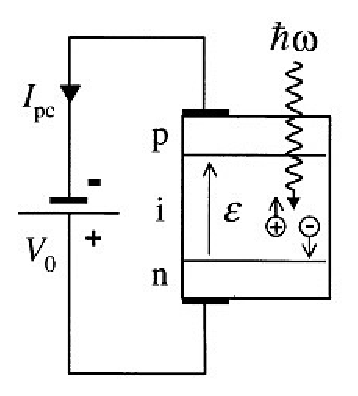
\includegraphics[width=25mm]{314.eps}
    \label{fig:3.14}
  \end{minipage}
 \\ [\intextsep]
Schematic diagram of a p-i-n photodiode. The diode is operated in reverse bias with a positive voltage $V_0$ applied to the n-region. This generates a strong DC electric field $\varepsilon$ across the i-region. Absorption of photons in the i-region creates free electrons $\ominus$ and holes $\oplus$ that are attracted to the n-region and p-regions respectively by the field. The carriers that reach the doped regions flow into the external circuit, thereby generating the photocurrent $I_{pc}$.}

Consider a photodiode of active length $l$ illuminated by a light beam of optical power $P$ and angular frequency $\omega$. The flux of photons per unit time on the detector is $P/\hbar\omega$. From the definition of the absorption coefficient given in eqn 1.4, we can deduce that the fraction of light absorbed in a length $l$ is equal to $(1-e^{-\alpha l})$, where $\alpha$ is the absorption coefficient at frequency $\omega$. Each absorbed photon generates one electron-hole pair, and we define the \textbf{quantum efficiency} $\eta$ as the fraction of these carriers that flow into the external circuit. The magnitude of the photocurrent $I_{pc}$ is thus given by:
\begin{equation}\label{equa:3.37}
  I_{pc}=e\eta\frac{P}{\hbar\omega}(1-e^{-\alpha l})
\end{equation}
We have assumed here that the top surface of the detector has been antireflection coated to prevent the wasteful reflection of incident photons. We have also assumed that the absorption in any layers above the active region is negligible.

The \textbf{responsivity} of the device is the ratio of the photocurrent $I_{pc}$ to the optical power $P$, and is given by:
\begin{equation}\label{equa:3.38}
  \text{Responsivity}=\frac{I_{pc}}{P}=\frac{\eta e}{\hbar\omega}(1-e^{-\alpha l})\quad \text{amps per watt}
\end{equation}
Equation 3.38 shows us that in order to obtain a large responsivity we need a high absorption and high quantum efficiency. Ideally, we would like to have both $\eta$ and $(1 - e^{-\alpha l})$ to be equal to unity, in which case the responsivity is simply $e/\hbar\omega$. This sets an upper limit on the responsivity that can be achieved.

For example, the maximum possible responsivity for a 2eV photon ($\lambda = 620 \mathrm{nm}$) is $0.5\mathrm{AW^{-1}}$. Well designed photodiodes can come quite close to this ideal figure.

The design of practical photodiodes is based on several criteria.

\begin{itemize}
  \item The choice of the semiconductor is made to optimize the responsivity while ensuring a fast response and low noise. The most fundamental criterion is that the band gap must be smaller than the photon energy. Having satisfied this criterion, we want $E_g$ to be as large as possible to minimize the noisy dark current that arises from the thermal excitation of electrons and holes across the gap. At the same time, we want a material in which the electron and hole mobilities are high so that the photogenerated carriers can be swept quickly across the device and give a fast response time.
  \item Materials with direct band gaps are better than those with indirect gaps because the absorption is higher. With typical values of $\alpha$ over $10^6 m^{-1}$ for direct absorption, the thickness of the active layer needs only to be $\sim\mathrm{1\mu m}$ to achieve very strong absorption. In an indirect gap semiconductor, greater thicknesses are required, which increases the constraints on the purity of the material. Furthermore, the direct gap materials can give faster response times because the thinner i-region reduces the transit time of the device.
  \item The top contact should be designed to transmit as much of the light into the i-region as possible. This means that the top contact should be made very thin. A better solution is to use different semiconductors for the p-njunction and i-region, such that the top contact has a larger band gap than the photons to be detected. This is possible with modem epitaxial semiconductor growth technology.
\end{itemize}
All these physical considerations have to be weighed against the manufacturing costs.

Table 3.2 gives a list of several common types of semiconductor photodetectors. Silicon is extensively used at visible and near-infrared wavelengths, despite the fact that the absorption is indirect. This choice is determined by the advanced technology of the silicon industry. Germanium detectors can be used out to $\mathrm{1.9\mu m}$, but for more demanding applications in the wavelength range $\mathrm{1-1.6\mu m}$, the \uppercase\expandafter{\romannumeral3}-\uppercase\expandafter{\romannumeral5} alloy semiconductor lnGaAs is becoming increasingly important. This is because it has a direct gap and also has a higher electron mobility than Ge, which means that fast, efficient detectors can be made for the telecommunications wavelengths of $\mathrm{1.3\mu m}$ and $\mathrm{1.5\mu m}$.

At wavelengths beyond $\mathrm{1.9\mu m}$, narrow gap semiconductors such as InAs or InSb have to be used. These long wavelength detectors invariably require cryogenic cooling to suppress the thermal dark currents and achieve good signal to noise ratios. The \uppercase\expandafter{\romannumeral2}-\uppercase\expandafter{\romannumeral6} alloy semiconductor HgCdTe is frequently used for wavelengths beyond $\mathrm{5\mu m}$. It has a band gap which can be varied according to the composition, and detectors with peak sensitivities in the range $\mathrm{5-14\mu m}$ are available. HgCdTe detectors are therefore able to cover several technologically important infrared wavelengths, especially $\mathrm{10.6\mu m}$, which corresponds to one of the infrared windows in the atmosphere and also to the emission lines of the $\mathrm{CO_2}$ laser. In Section 6.7 of Chapter \ref{chap:6} we will describe an alternative detector for $\mathrm{10.6\mu m}$ which has recently been developed using GaAs quantum wells. These quantum well detectors operate on a different principle to the interband detectors described here.

\subsection{Photoconductive devices}

An alternative way to make a semiconductor photodetector is to use the photoconductive effect. This relies on the change of the conductivity of the material when illuminated by light. The conductivity is proportional to the density of free electrons and holes. The conductivity therefore increases due to the generation of free carriers after absorption of photons by interband transitions.

The devices consist of a sample with contacts at the ends so that a constant DC current can flow through the semiconductor between the contacts. The resistance between the contacts decreases upon illumination. This alters the voltage dropped across the device, and hence provides the detection mechanism. Photoconductive detectors are simpler to make than photodiodes, but tend to have slow response times.

\subsection{Photovoltaic devices}

Semiconductor photodiodes can also be operated in photovoltaic mode. In this mode of operation, the device does not have an external power supply. Instead it generates a photovoltage when irradiated by light. This in turn can be used to generate electrical power in an external load. This is the basis of operation of \textbf{solar cells}, which convert sunlight into electrical power.

The operating principle of a photovoltaic device relies on the relationship between the photocurrent and the applied bias in a photodiode. The photocurrent is sensitive to the bias because it affects the electric field $\varepsilon$ across the depletion region. As explained in Appendix D, the field strength can be quite large even when the external bias is zero. This is because of the alignment of the Fermi levels in the p- and n-regions, which produces a voltage drop across the depletion region called the built-in voltage $V_{bi}$. The magnitude of $V_{bi}$ is approximately equal to $E_g/e$. A forward bias approximately equal to $V_{bi}$ must therefore be applied before $\varepsilon$ drops to zero. The diode will produce a photocurrent on illumination provided that there is a field to sweep out the electrons and holes. Thus photocurrents can be produced at zero bias and even in forward bias, provided the forward bias voltage is less than $V_{bi}$.

Let us suppose that we replace the battery in Fig. 3.14 with an electrical load of resistance $R$. The voltage on the diode in the dark is zero. If the diode is illuminated, a photocurrent will be generated because the field due to the built-in voltage sweeps the carriers out of the i-region. This photocurrent flows through the load and the device therefore converts optical power to electrical  power. The magnitude of the electrical power is $I_{pc}^2R$. The direction of the photocurrent is such that the photovoltage $I_{pc}R$ across the load puts the diode in forward bias. Thus if the illumination level is increased from zero, the photocurrent will saturate as the photovoltage approaches $V_{bi}$. This limits the maximum amount of electrical power that can be generated. At present, the maximum power conversion efficiency achieved in a silicon solar cell is in the range $10-25\%$.

\section*{Chapter Summary}

\definecolor{shadecolor}{rgb}{1.0,0.9,0.9}
\begin{shaded}
\begin{itemize}
  \item Interband transition occur when electrons jump to an excited state band by absorption of photons. The absorption process may be considered as the creation of an electron-hole pair.
  \item Interband absorption is only possible if the photon energy exceeds the band gap energy $E_g$. The absorption spectrum therefore shows a threshold at $E_g$.
  \item The absorption rate for direct transitions is proportional to the product of the joint density of states and the square of the electric dipole matrix element.
  \item The photon wave vector is negligible compared to that of the electron, and so the electron wave vector is unchanged in a direct transition. Direct transitions are represented by vertical arrows on $E-k$ band diagrams.
  \item The frequency dependence of the absorption edge of a direct gap semiconductor at $E_g$ is given by eqn 3.25. At higher frequencies, the absorption coefficient is determined by the detailed frequency dependence of the joint density of states. The absorption is particularly high at critical points.
  \item The application of an external electric field results in non-zero absorption below the band gap through the Franz-Keldysh effect. The application of a magnetic field causes the absorption edge to shift to higher energy.
  \item Interband transitions in indirect gap materials involve the absorption or emission of a phonon to conserve momentum in the process. Indirect absorption is much weaker than direct absorption since it is a second-order process.
  \item The frequency dependence of the absorption edge in an indirect gap material is given by eqn 3.35. This is different to that observed in direct gap semiconductors, and provides a way for determining the nature of the band gap experimentally.
  \item The absorption of light by interband transitions can be used to make photodetectors. The detection mechanism is based on the generation of a photocurrent or the increase of the conductivity after absorption of photons with energies greater than the band gap.
\end{itemize}
\end{shaded}
\section*{Further Reading}
The electronic states of solids are covered in the companion book of this series by Singleton (2001). They are also covered in all general solid state texts, for example Bums (1985), Ibach and Luth (1995) or Kittel (1996), and in more detail by Harrison (1999).

Detailed information on the interband absorption of semiconductors may be found in Klingshirn (1995), Pankove (1971), Seeger (1997), or Yu and Cardona (1996). Introductory treatments of the application of group theory to interband transitions can be found in Klingshirn (1995) or Yu and Cardona (1996). Yu and Cardona (1996) also give the derivation of the frequency dependence of the absorption coefficient in an indirect gap semiconductor (eqn 3.35).

The Franz-Keldysh effect is described in Klingshirn (1995), Seeger (1997), or Yu and Cardona (1996). Yu and Cardona (1996) explain the use of electroreftectance to determine band structure parameters, while Seeger ( 1997) gives a good discussion of the effect of magnetic fields on the band edge absorption.

The physics of semiconductor photodetectors is described in more detail in Bhattacharya (1997), Chuang (1995), Sze (1985), Wilson and Hawkes (1998), or Yariv (1997). Sze (1985) gives a good discussion of solar cells.

\chapter{Excitons}\label{chap:4}
\definecolor{shadecolor}{rgb}{0.9,0.9,0.9}
\begin{shaded}

In the previous chapter we discussed the absorption of photons by interband transitions. We saw that this process creates an electron in the conduction band and a hole in the valence band, but we neglected the effects of the mutual Coulomb attraction between them. As we will see in this chapter, the Coulomb interaction can give rise to the formation of new excitations of the crystal called excitons. These excitons have interesting optical properties and are important for optoelectronic applications.

We will encounter excitons in several different contexts throughout this book. In this chapter we will concentrate mainly on their effects on the absorption edge of bulk semiconductors. In Chapter \ref{chap:6} we will see how the excitonic effects can be enhanced by forming quantum well structures containing very thin layers of direct gap semiconductors such as GaAs. In Chapter \ref{chap:8} we will see how the excitonic effects have a strong influence on the optical properties of molecular materials. Finally, in Chapter \ref{chap:11} we will briefly study how the presence of excitons can give rise to useful nonlinear optical properties in bulk and quantum well semiconductors.
\end{shaded}

\section{The Concept of Excitons}

The absorption of a photon by an interband transition in a semiconductor or insulator creates an electron in the conduction band and a hole in the valence band. The oppositely charged particles are created at the same point in space and can attract each other through their mutual Coulomb interaction. This attractive interaction increases the probability of the formation of an electron-hole pair, and therefore increases the optical transition rate. Moreover, if the right conditions are satisfied, a bound electron-hole pair can be formed. This neutral bound pair is called an exciton. In the simplest picture, the exciton may be conceived as a small hydrogenic system similar to a positronium atom with the electron and hole in a stable orbit around each other.

Excitons are observed in many crystalline materials. There are two basic types:
\begin{itemize}
  \item \textbf{Wannier-Mott excitons}, also called \textbf{free excitons};
  \item \textbf{Frenkel excitons}, also called \textbf{tightly bound excitons}.
\end{itemize}
The Wannier-Mott excitons are mainly observed in semiconductors, while the Frenkel excitons are found in insulator crystals and molecular crystals.

The two generic types of exciton are illustrated schematically in Fig. 4.1. The diagrams show an electron and hole orbiting around each other within a crystal. The Wannier-Mott type excitons have a large radius that encompasses many atoms, and they are delocalized states that can move freely throughout the crystal; hence the alternative name of \lq free\rq excitons. Frenkel excitons, by contrast, have a much smaller radius which is comparable to the size of the unit cell. This makes them localized states which are tightly bound to specific atoms or molecules; hence their alternative name of \lq tightly bound\rq excitons. Tightly bound excitons are much less mobile than free excitons, and they have to move through the crystal by hopping from one atom site to another.

Stable excitons will only be formed if the attractive potential is sufficient to protect the exciton against collisions with phonons. Since the maximum energy of a thermally excited phonon at temperature $T$ is $\sim k_BT$, where $k_B$ is Boltzmann's constant, this condition will be satisfied if the exciton binding energy is greater than $k_BT$. Wannier-Mott excitons have small binding energies due to their large radius, with typical values of around 0.01 eV. Since $k_BT\sim 0.025$eV at room temperature, the excitons are only observed clearly at cryogenic temperatures in many materials. Frenkel excitons, on the other hand, have larger binding energies of the order 0.1-1 eV, which makes them stable at room temperature.

In the sections that follow, we will first describe the basic properties of free excitons, and then study how they are affected by external electric and magnetic fields. We will then discuss the interactions between excitons, which are the basis for the nonlinear optical properties of excitons discussed in Chapter \ref{chap:11}. We close the chapter with a brief discussion of the optical properties of Frenkel excitons.

\section{Free Excitons}
\subsection{Binding energy and radius}
In a free exciton, the average separation of the electrons and holes is much greater than the atomic spacing, as shown in Fig. 4.l(a). This is effectively the definition of a Wannier exciton, and it specifies more accurately what is meant by saying that the free exciton is a weakly bound electron-hole pair. Since the electron-hole separation is so large, it is a good approximation to average over the detailed structure of the atoms in between the electron and hole and consider the particles to be moving in a uniform dielectric material. We can then model the free exciton as a hydrogenic system similar to positronium.

We know from atomic physics that the motion of hydrogenic atoms splits into the centre of mass motion and the relative motion. (See Exercise 4.1.) The centre of mass motion describes the kinetic energy of the atom as a whole, while the relative motion determines the internal structure. The energies of the bound states can be determined by finding the eigenvalues of the Schr\"{o}dinger equation for the relative motion, or alternatively by using approximation techniques such as the variational method. (See Exercises 4.2-4.4). The main results are, however, well explained by using the Bohr model (cf. Exercise 4.5), and this is the procedure we will adopt here.

In applying the Bohr model to the exciton, we must take account of the fact that the electron and hole are moving through a medium with a high dielectric constant Er. We must also remember that the reduced mass $\mu$ will be given by eqn \ref{equa:3.22}, instead of the value of $0.9995 m_0$ that applies to the electron-proton system in a hydrogen atom. With these two qualifications, we can then just use the standard results of the Bohr model. The bound states are characterized by the principal quantum number $\texttt{n}$. The energy of the \texttt{n}th level relative to the ionization limit is given by
\begin{equation}\label{equa:4.1}
  E(\texttt{n})=-\frac{\mu}{m_0}\frac{1}{\epsilon_r^2}\frac{R_H}{\texttt{n}^2}
\end{equation}
where $R_H$ is the Rydberg constant of the hydrogen atom (13.6 eV). The quantity $R_X = (\mu/m_o\epsilon_r^2)R_H$ introduced here is the exciton Rydberg constant. The radius of the electron-hole orbit is given by
\begin{equation}\label{equa:4.2}
  r_{\texttt{n}}=\frac{m_0}{\mu}\epsilon_r\texttt{n}^2a_H=\texttt{n}^2a_X
\end{equation}
where $a_H$ is the Bohr radius of the hydrogen atom ($5.29\times 10^{-11} m$) and $a_X = (m_0\epsilon_r/\mu)a_H$ is the exciton Bohr radius. Equations \ref{equa:4.1} and \ref{equa:4.2} show that the ground state with $\texttt{n} = 1$ has the largest binding energy and smallest radius. The excited states with $\texttt{n > 1}$ are less strongly bound and have a larger radius.

Table 4.1 lists the exciton Rydberg constant and Bohr radius for a number of direct gap III-V and II-VI semiconductors. A general pattern is easily noticed in the data, namely that $R_X$ tends to increase and $a_X$ to decrease as $E_g$ increases. This is explained by the fact that $\epsilon_r$ tends to decrease and $\mu$ to increase as the band gap increases. From eqns \ref{equa:4.1} and \ref{equa:4.2}, we see that this causes an increase in the exciton binding energy and a decrease in the radius. In insulators with band gaps greater than about 5 eV, $a_X$ becomes comparable to the unit cell size, and the Wannier model is no longer valid. At the other extreme, $R_X$ is so small in narrow gap semiconductors such as InSb that it is difficult to observe any free exciton effects at all. Hence, free exciton behaviour is best observed in semiconductors with medium-sized band gaps in the range $\sim 1-3 $eV.

\subsection{Exciton absorption}

Free excitons are typically observed in direct gap semiconductors such as GaAs. They are created during direct optical transitions between the valence and conduction bands. As discussed in Section 3.2 this creates an electron-hole pair in which the electron and hole have the same $\mathbf{k}$ vector.

Excitons can only be formed if the electron and hole group velocities $v_e$ and $v_h$ are the same. This is a necessary condition for the electrons and holes to be able to move together as a bound pair. The group velocity of an electron in a band is given by (see eqn C.4):
\begin{equation}\label{equa:4.3}
  v_g=\frac{1}{\hbar}\frac{\partial E}{\partial \mathbf{k}}
\end{equation}
This implies that the condition $v_e=v_h$ can only be satisfied if the gradients of the conduction and valence bands are the same at the point of the Brillouin zone where the transition occurs. All bands have zero gradient at the zone centre. Hence we can form excitons during a direct transition at $\mathbf{k} = 0$. In a direct gap semiconductor, these transitions correspond to photon energies of $E_g$ (cf. eqn \ref{equa:3.23}). Therefore we expect to observe strong excitonic effects in the spectral region close to the fundamental band gap.

The energy of the exciton created in a direct transition at $k = 0$ is equal to the energy required to create the electron-hole pair, namely $E_g$, less the binding energy due to the Coulomb interaction, which is given by eqn \ref{equa:4.1}. Hence the energy of the exciton will be given by:
\begin{equation}\label{equa:4.4}
  E_{\texttt{n}}=E_g-\frac{R_X}{\texttt{n}^2}
\end{equation}
Whenever the photon energy is equal to $E_{\texttt{n}}$, excitons can be formed. The probability for the formation of excitons is expected to be high, because it is energetically favourable for the exciton states to be formed compared to free electron-hole pairs. Therefore we expect to observe strong optical absorption lines at energies equal to $E_{\texttt{n}}$. These will appear in the optical spectra at energies just below the fundamental band gap. The band edge absorption spectrum expected when excitonic effects are included is illustrated schematically in Fig. 4.2.
\marginnote{
\begin{minipage}{\textwidth}
    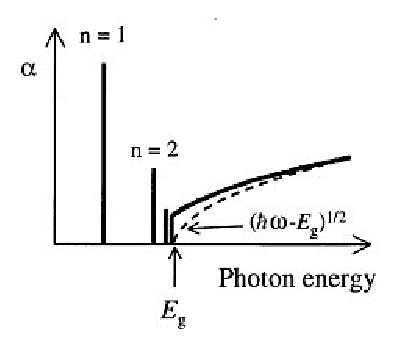
\includegraphics[width=30mm]{42.eps}
    \label{fig:4.2}
  \end{minipage}
 \\ [\intextsep]
Band edge absorption spectrum for a direct gap semiconductor with excitonic effects included. The dashed line shows the expected absorption when the excitonic effects are ignored.}

Free excitons can only be observed in the absorption spectrum of very pure samples. This is because impurities release free electrons and holes that can screen the Coulomb interaction in the exciton and thereby strongly reduce the binding forces. For this reason, excitonic effects are not usually observed in doped semiconductors or metals, since they contain a very high density of free carriers. Charged impurities also generate electric fields, which tend to ionize the excitons, as discussed in Section 4.3.1.

\subsection{Experimental data for free excitons in GaAs}

Figure 4.3 gives experimental data for the excitonic absorption of undoped GaAs between 21 K and 294 K. As expected, the data show strong absorption lines at photon energies just below the fundamental band gap of GaAs. At 21 K a sharp line is observed just below the direct absorption edge. This corresponds to the $\texttt{n} = 1$ exciton. The line is too broad to permit observation of any of the excited states. As the temperature is increased, the band gap shifts to lower energy and the exciton line weakens. At room temperature where $k_BT\gg R_X$, the exciton line has completely gone.

The spectrum at 185 K shows a weak exciton line at the band edge even though $k_BT$ is almost four times greater than $R_X$. This indicates that the criterion for exciton stability used in Example 4.1(iii), namely $k_B<R_X$, is too stringent. The main mechanism that causes dissociation of excitons is collisions with longitudinal optic (LO) phonons. As the probability of such collisions increases, the lifetime of the excitons shortens. This leads to a corresponding broadening of the exciton line in the absorption spectrum. In GaAs, the relevant LO phonon has an energy of $\mathrm{35 meV}$, which has a thermal occupation of $11\%$ at 185 K. (cf. eqn 3.36.) There are therefore still relatively few LO phonons in the crystal at this temperature, and so the collisional broadening does not yet exceed $R_X$, and the exciton line is just resolved.

The dashed line in Fig. 4.3 shows the frequency dependence of the absorption edge expected if excitonic effects are ignored. This line is obtained from eqn 3.25 with a value of 1.425 eV for $E_g$, which is appropriate for GaAs at 294 K. We see that the fit to the data is not good. This tells us that the Coulomb interaction between the electron and hole still enhances the absorption rate considerably, even though there are no clear exciton lines observed in the spectrum.

Figure 4.4 shows more recent data for the excitonic absorption of ultra pure GaAs at 1.2 K. The data clearly show the hydrogen-like energy spectrum of the exciton in the vicinity of the band gap. The exciton lines are more clearly resolved in this data set than in Fig. 4.3 because the temperature is lower and the sample purity is superior. As discussed above, the presence of impurities leads to screening of the Coulomb interaction by free carriers, while lower temperatures reduce the thermal broadening of the absorption lines.

Three exciton states can be clearly identified in the absorption spectrum shown in Fig. 4.4. The energies of the $\texttt{n} = 1$, $\texttt{n} = 2$ and $\texttt{n} = 3$ excitons are 1.5149 eV, 1.5180 eV, and 1.5187 eV respectively. These energies fit eqn \ref{equa:4.4} very well with $E_g=1.5191 \mathrm{eV}$ and $R_X = 4.2 \mathrm{meV}$. This value of $E_g$ agrees well with other measurements, while the experimental figure of $4.2 \mathrm{meV}$ for $R_X$ is in excellent agreement with the value calculated in Example 4.1.

\marginnote{
\begin{minipage}{\textwidth}
    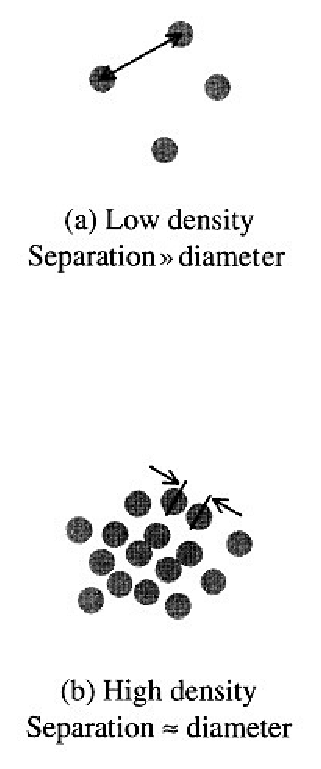
\includegraphics[width=30mm]{46.eps}
    \label{fig:4.6}
  \end{minipage}
 \\ [\intextsep]
Distribution of the free excitons within a crystal. (a) Low densities: the excitons are random distributed throughout the excitation volume and the interexciton separation is large. (b) High densities: the wave functions overlap when the exciton-exciton separation becomes comparable to the exciton diameter.}

\section{Free Excitons in External Fields}

Free excitons are bound together by the electrostatic attraction between the negative electron and the positive hole. External electric and magnetic fields perturb the system through the forces exerted on the charged particles. The effects of these perturbations are discussed here, using the excitons in GaAs as an example.

\subsection{Electric fields}

When a DC electric field $\varepsilon$ is applied to an exciton, the oppositely charged electrons and holes are pushed away from each other. It is shown in Exercise 4.10 that the order of magnitude of the electric field between the electron and hole in the ground state exciton is equal to $2R_X/ea_X$. If $\varepsilon$ exceeds this value, the exciton will break apart. This effect is known as \textbf{field ionization}.

Electric fields are applied to excitons by incorporating the semiconductor as the i-region in a p-i-n diode structure, as discussed in Appendix D. The field strength across the i-region when a bias voltage $V_0$ is applied is given by eqn D.3 as:
\begin{equation}\label{equa:4.5}
  \varepsilon=\frac{|V_{bi}-V_0|}{l_i}
\end{equation}
where $V_{bi}$ is the built-in voltage of the diode and $l_i$ is the intrinsic region thickness. The sign convention is such that positive $V_0$ corresponds to forward bias.

In a typical GaAs p-i-n diode, the i-region thickness is about $1 \mu m$, and $V_{bi}$ is about 1.5 V. Equation 4.5 then tells us that $\varepsilon$ is $1.5\times 10^6 V m^{-1}$ at zero bias. At the same time we see from Table 4.1 that in GaAs $2R_X/ ea_X$ is of order $6\times 10^5 Vm^{-1}$, which is substantially less than the field strength at $V_0 = 0$. We would therefore expect the excitons to be ionized even before we apply
bias to the diode.

Figure 4.5 shows experimental data for the field ionization of free excitons in a GaAs p-i-n diode with $l_i = 1.0\mu m$ at 5 K. In this experiment, the diode is illuminated with light, and the photocurrent generated at a given voltage and wavelength is recorded. The solid line is the photocurrent recorded in \lq flat band conditions\rq ($V_0 = + 1.44\mathrm{V}$, $\varepsilon\approx0$), while the dashed line is for $V_0 = + 1.00 \mathrm{V}$, where $\varepsilon\approx 5 \times 10^5 V m^{-1}$. In the flat band case we observe a well-resolved exciton line at 1.515 eV. However, once we reduce the bias by only a very small amount, we rapidly approach the ionization field, and the exciton broadens significantly. At zero bias (not shown), we are well above the ionization field, and no exciton lines are resolved in the spectrum.

From the discussion above, it is clear that excitonic effects do not play a large part in the physics of bulk semiconductor diodes. The excitons will only be observed over a small range of forward bias voltages just less than $V_{bi}$. Therefore, the physics of bulk semiconductors in electric fields is dominated more by the effect of the field on the band states, namely the Franz-Keldysh effect discussed in Section 3.3.5. As we will see in Chapter \ref{chap:6}, this is not the case for the enhanced free excitons in GaAs quantum wells. These show very interesting electric field effects even at room temperature.

\subsection{Magnetic fields}

The application of a magnetic field perturbs the free excitons by applying magnetic forces to the electron and hole. The strength of the perturbation is set by the exciton cyclotron energy $\hbar\omega$, which is given by
\begin{equation}\label{equa:4.6}
  \hbar\omega=\hbar\frac{eB}{\mu}
\end{equation}
where $B$ is the magnetic flux density. This is similar to the formula for individual electrons given in eqn 3.27, except that the reduced electron-hole effective mass $\mu$ appears instead of the individual electron mass.

The behaviour can be divided into the weak and strong field  limits, with the transition point set by the ratio of the exciton Rydberg energy to the cyclotron energy. If $R_X\gg \hbar\omega_c$, we are in the weak field regime, whereas $R_X\ll\hbar\omega_c$ corresponds to the strong field regime. In GaAs, the transition between the two limits occurs around 2 T for the $\texttt{n}= 1$ exciton: see Exercise 4.12.

In the weak field limit we treat the magnetic field as a perturbation on the excitons. The ground state of a hydrogen atom has no net magnetic moment because it is spherically symmetric. Thus the interaction between the $\texttt{n} = 1$ exciton and the $B$-field will be described by diamagnetic effects. The diamagnetic energy shift is given by (see Exercise 4.13):
\begin{equation}\label{equa:4.7}
  \delta E=+\frac{e^2}{12\mu}r_{\texttt{n}}^2B^2.
\end{equation}
The shift is positive because Lenz's law tells us that the field induces a magnetic moment that opposes the applied field. This induced dipole then interacts with the field to give an energy shift proportional to $+B^2$.

In the strong field limit, the interaction of the electrons and holes with the field is stronger than their mutual Coulomb interaction. We therefore consider the Landau energy of the individual electrons and holes first, as in Section 3.3.6. We then add on the Coulomb interaction as a small perturbation. The details of this analysis are beyond the scope of this book. The end result is that the excitonic effects cause a small shift in the energies of the optical transitions between the Landau levels.

\section{Free Excitons at High Densities}
Wannier excitons behave as if they are hydrogen-like atoms moving freely through the crystal. The atoms in a gas of hydrogen are agitated by thermal motion and interact with each other whenever they get close together. The simplest type of interaction is the tendency to form the $\mathrm{H_2}$ molecule, but other phenomena such as Bose-Einstein condensation are also possible. Excitons show a similar variety of phenomena such as the tendency to form molecules or condense to a liquid phase. The type of behaviour observed in any one material depends very much on the conditions that apply and the details of the interactions between the excitons.

We first consider an experiment in which we take a powerful laser and tune it to one of the exciton absorption lines. The laser creates excitons in the sample, with a density that is proportional to the laser power. At low powers, the density of the excitons is small, and the separation between the excitons is large, as sketched in Fig. 4.6(a). The exciton-exciton interactions are negligible in these conditions. As the power is increased, the density of excitons increases. Eventually, the density will be high enough that the exciton wave functions begin to overlap, as sketched in Fig. 4.6(b). At this point, we expect that the exciton-exciton interactions will become very significant.

We can see from Fig. 4.6(b) that exciton wave function overlap occurs when the exciton-exciton distance is equal to the exciton diameter. The density at which this occurs is called the \textbf{Mott density} $N_{Mott}$· It is given approximately by the inverse volume of the exciton:
\begin{equation}\label{equa:4.8}
  N_{Mott}\approx\frac{1}{\frac{4}{3}\pi r_{\texttt{n}}^3}
\end{equation}
From Table 4.1 and eqn 4.2, we find that the Mott density for the $\texttt{n} = 1$ excitons in GaAs is $1.1\times10^{23} \mathrm{m^{-3}}$. This density is easily achievable with a focussed laser beam.

When the exciton density approaches $N_{Mott}$ , a number of effects can occur. In GaAs the collisions between the excitons cause the exciton gas to dissociate into an electron-hole plasma. This causes exciton broadening with a reduction in the absorption strength. Figure 4.7 shows the absorption coefficient at the $\texttt{n} = 1$ exciton in GaAs at 1.2 K at three different excitation powers. The weakening and broadening of the exciton line as the carrier density is increased is clearly observed in the data. The density at which these effects occur agrees well with the value of $1.1\times 10^{23} \mathrm{m^{-3}}$ given by eqn \ref{equa:4.8}. The saturation of the exciton absorption with increasing power is an example of a nonlinear optical effect: the absorption coefficient depends on the intensity of the light. We will return to discuss applications of these nonlinear effects in Section 11.4.3 of Chapter \ref{chap:11}.

Another effect that can be observed at high exciton densities in other materials is the formation of exciton molecules called \textbf{biexcitons}. This is the equivalent process to the formation of an $\mathrm{H_2}$ molecule from two isolated hydrogen atoms. Biexcitons have been observed in a number of compound semiconductors, including CdS, ZnSe, ZnO and especially copper chloride. CuCl has a band gap at 3.40 eV, and the ground state exciton is observed at 3.20 eV, implying that $R_X = 0.2$ eV. At high densities, a new feature is observed in the absorption spectrum at 3.18 eV. This is attributed to biexciton formation. The energy difference between the two features tells us that the binding energy of the biexciton is 0.02 eV. Attempts to observe biexcitons in materials like GaAs have been hindered by the nonlinear saturation effects described above.

In silicon and germanium at high densities, yet another effect occurs. At low densities the excitons may be considered to be in a gaseous phase. As the density increases, the excitons condense to form a liquid. The liquid phase manifests itself in the formation of \textbf{electron-hole droplets}, which are observed in the recombination radiation of the excitons at high densities. The droplet appears as a broad feature at lower energy than the free excitons.

The final high density effect that we consider here is Bose-Einstein condensation. At high temperatures, the particles in a non-interacting boson gas are distributed between the possible energy levels of the system according to Bose-Einstein statistics. As the temperature is lowered, the distribution undergoes a radical range, and a macroscopic number of particles accumulate in the ground state. The critical temperature Tc at which this occurs is given by:
\begin{equation}\label{equa:4.9}
  N=2.612\left(\frac{mk_BT_c}{2\pi\hbar^2}\right)
\end{equation}
where $N$ is the number of particles per unit volume and $m$ is the particle mass. At $T_c$ the thermal de Broglie wavelength is comparable to the interparticle separation, and quantum effects are to be expected. (See Exercise 4.16.)

Bose-Einstein condensation has been observed in many boson systems. One of the best studied examples is liquid helium. In this case, $N$ is fixed, and eqn \ref{equa:4.9} predicts a phase transition as the liquid is cooled through Tc at 2.2 K. However, the physics of Bose-Einstein condensation is complicated in liquid helium by the strong interactions between the atoms. To achieve pure Bose­Einstein condensation behaviour, we require that the interactions between the bosons are negligible. This suggests that we need highly dilute gaseous sys­ tems such that the interparticle separation is very large. However, from eqn \ref{equa:4.9} we see that the transition temperature for such a dilute system would be very low. It has been an outstanding recent achievement of atomic physics to suc­ ceed in observing Bose-Einstein condensation in extremely dilute gases of atoms at temperatures below $1\mathrm{\mu K}$.

Excitons consist of two spin $\frac{1}{2}$ particles, and so their total spin is either $0$ or $1$. This means that they are bosons. There have been many attempts to study condensation phenomena, but practically all of the claimed observations have been disputed. It is actually very difficult to prove definitively that conden­ sation has occurred. Two of the most promising candidate systems that have been  studied to date are the spin-$0$ excitons in copper oxide ($\mathrm{Cu_2O}$) and the biexcitons in CuCl.

\section{Frenkel Excitons}

The free exciton model that leads to eqns \ref{equa:4.1} and \ref{equa:4.2} breaks down when the predicted radius becomes comparable to the interatomic spacing. This occurs in large band gap materials with small dielectric constants and large effective masses. In these materials we observe Frenkel excitons rather than Wannier excitons.

Frenkel excitons are localized on the atom site at which they are created, as shown in Fig. 4.l(b). The excitons may therefore be considered as excited states of the individual atoms or molecules on which they are localized. They have very small radii and correspondingly large binding energies, with typical values ranging from about 0.1 eV to several e V. This means that Frenkel excitons are usually stable at room temperature. The excitons can propagate through the crystal by hopping from atom site to site in the same way that spin excitations propagate through crystals as magnon waves.

The theoretical treatment of Frenkel excitons requires techniques more akin to atomic or molecular physics than solid state physics. There is no simple model similar to the one that led to eqns \ref{equa:4.1} and \ref{equa:4.2} for free excitons. The calculation of the exciton energies usually follows a tight binding approach, in order to emphasize the correspondence to the atomic or molecular states from which the excitons are derived. The calculation is further complicated by the fact that the coupling between the excitons and the crystal lattice is usually very strong. This leads to \lq self-trapping\rq effects, in which the exciton produces a local distortion of the lattice, which then causes further localization of the exciton wave functions.

Frenkel excitons have been observed in many inorganic and organic materials. The properties of some of the more widely studied crystals are described briefly below.

\subsection{Rare gas crystals}

The rare gases from group VIII of the periodic table, namely neon, argon, krypton and xenon, crystallize at cryogenic temperatures. The band gap ranges from 21.6 eV in neon to 9.3 eV in xenon. Neon in fact has the largest band gap of any crystal known in nature. The excitonic absorption of these materials has been thoroughly studied, and the results are summarized in Table 4.2. The exciton transitions all occur in the vacuum ultraviolet spectral range, and the binding energies are very large.

It has been found experimentally that there is a close correspondence between the $\texttt{n} = 1$ exciton energies in the crystals and the optical transitions of the isolated atoms. For example, the energy of the $\texttt{n} = 1$ exciton in xenon crystals coincides almost exactly with the lowest energy absorption line of xenon atoms in the gaseous phase, namely the $5p^6\rightarrow5p^56s$ transition. This underlines the point made earlier that the localized nature of the Frenkel excitons makes them equivalent to excited states of the individual atoms or molecules. This correspondence gets weaker for the excitons with larger values of $\texttt{n}$. As the radius increases with $\texttt{n}$, the excitons become more and more delocalized, and it eventually becomes valid to use the Wannier model.

\subsection{Alkali halides}

Frenkel excitons are readily observable in the optical spectra of alkali halide crystals. These have large direct band gaps in the ultraviolet spectral region ranging from 5.9 eV in NaI to 13.7 eV in LiF. LiF has the widest band gap of any practical optical material: only argon and neon crystals have larger band gaps, but neither of these are solids at room temperature.

Table 4.3 lists the band gap of selected alkali halide crystals, together with the energy and binding energy of the $\texttt{n}=1$ exciton. The data show that Eg tends to increase with decreasing anion and cation size. The exciton binding energy follows a similar general trend. Detailed spectroscopy has established that the excitons are localized at the negative (halogen) ions.

Figure 4.8 shows the absorption spectrum of two representative alkali halide crystals at room temperature, namely NaCl and LiF. Both spectra show a strong excitonic absorption line below the band gap. The binding energies are 0.8 eV and 1.9 eV respectively. These values are well above $k_BT$ at room temperature, which explains why the excitons are observed so strongly. The fine structure of the excitons due to the excited states can be observed by cooling the crystals. Note that the absorption coefficient at the exciton lines is extremely large, with values over $10^8\mathrm{m}^{-1}$ in both materials.

\subsection{Molecular crystals}
Frenkel excitons can be observed in many molecular crystals and organic thin film structures. In most cases, there is a very strong correspondence between the optical transitions of the isolated molecules and the excitons observed in the solid state. This is a consequence of the fact that the molecular crystals are held together by relatively weak van der Waals forces, so that the molecular levels are only weakly perturbed when condensing to the solid state.

Figure 4.9 shows the fundamental absorption edge of pyrene crystals at room temperature. The pyrene molecule has a composition of $\mathrm{C_{16}H_{10}}$ and is an example of an aromatic hydrocarbon, that is, a carbon-hydrogen compound based on benzene rings. The 4-ring structure of pyrene is given in the inset. The absorption spectrum shows a clear excitonic peak at 3.29 eV. Other aromatic hydrocarbons such as anthracene ($\mathrm{C_{14}H_{10}}$) also show very strong excitonic effects, but the optical spectra are more complicated because of the strong coupling to the vibrational modes of the molecule. These effects will be discussed in more detail in Section 8.4 in Chapter 8. The pyrene spectrum is relatively simple because the 4-ring structure makes the molecule very rigid and reduces the effects of the vibrational coupling.

Frenkel excitons are also very important in conjugated polymers, such as polydiacetylene (PDA). Single crystals of PDA can be grown, but the optical properties are often studied by using amorphous films coated onto glass substrates. The strong excitonic effects in conjugated polymers have acquired considerable technological significance in recent years, following the development of organic light emitting diodes for use in display technology. The optical properties of organic semiconductors such as PDA will be discussed in more detail in Sections 8.5 and 8.6 of Chapter \ref{chap:8}.

\section*{Chapter Summary}
\definecolor{shadecolor}{rgb}{1,0.9,0.9}
\begin{shaded}
\begin{itemize}
  \item Excitons are electron-hole pairs bound together in stable orbits by the mutual Coulomb attraction between them.
  \item There are two types of excitons. Wannier (free) excitons have a large radius and move freely throughout the crystal. Frenkel (tightly bound) excitons are localized on individual atoms sites.
  \item The properties of free excitons can be calculated by treating them as hydrogen-like atoms. The binding energies and radii are given by eqns \ref{equa:4.1} and \ref{equa:4.2} respectively.
  \item Free excitons are observed in semiconductors at photon energies just below $E_g$. They have fairly small  binding energies, and are observed most clearly ar low temperatures. They are easily ionized by electric fields.
  \item Free excitons can interact with each other, and they show a rich variety of phenomena at high densities due to the exciton-exciton interactions.
  \item Frenkel extitons have very small radii and large binding energies. They are easily observed at room temperature in insulator crystals and molecular materials. There is a strong correspondence between the excitons observed in the solid state and the excited states of the individual atoms or molecules of which the solid is composed.
\end{itemize}
\end{shaded}

\section*{Further Reading}
Supplementary reading on excitons may be found in most of the standard solid state texts such as Burns ( 1985) or Kittel ( 1996). More detailed information on free excitons in semiconductors may be found in Klingshirn (1995), Pankove (1971), Seeger (1997), or Yu and Cardona (1996).

Dexter and Knox (1965) is a classic text on excitons, while Rashba and Sturge ( 1982) is a more recent authoritative reference work. Reynolds and Collins (1981) give a good overview of excitonic physics, while Song and Williams (1993) give a thorough discussion of the properties of Frenkel excitons.

An overview of high density exciton effects may be found in Klingshirn (1995). The general phenomenon of Bose-Einstein condensation is discussed in most texts on statistical mechanics, for example, Mandl (1988). Griffin \textit{et al.} (1995) give a review of measurements of condensation in a wide variety of systems. Reviews of Bose condensation effects in atomic systems may be found in Wieman (1997) or Ketterle (1999).

\chapter{Luminescence}\label{chap:5}
\definecolor{shadecolor}{rgb}{0.9,0.9,0.9}
\begin{shaded}

In Chapter \ref{chap:3} we considered how light can be absorbed in solids by exciting interband transitions. Then in Chapter \ref{chap:4} we considered how the absorption spectrum is modified by the interactions that lead to the formation of excitons. We now consider the reverse process in which electrons in an excited state drop to lower levels by emitting photons. This is the solid state equivalent to light emission in atoms by spontaneous emission, which is reviewed in Appendix B.

The physical mechanisms responsible for light emission in solids vary considerably from material to material. In this chapter we will start by giving a few general principles that apply to all materials, and then focus on the emission of light by interband transitions in bulk semiconductors. This will provide the framework for discussing the light emission processes in semiconductor quantum wells in Chapter \ref{chap:6}, and will also serve as a general introduction to the light emission processes in other types of materials.
\end{shaded}

\section{Light Emission in Solids}
Atoms emit light by spontaneous emission when electrons in excited states drop down to a lower level by radiative transitions. In solids the radiative emission process is called \textbf{luminescence}. Luminescence can occur by a number of mechanisms, but in this book we will mainly be considering just two:
\begin{itemize}
  \item \textbf{Photoluminescence}: the re-emission of light after absorbing a photon of higher energy.
  \item \textbf{Electroluminescence}: the emission of light caused by running an electrical current through the material.
\end{itemize}

The physical processes involved in both photoluminescence and electroluminescence are more complicated than those in absorption. This is because the generation of light by luminescence is intimately tied up with the energy relaxation mechanisms in the solid. Furthermore, the shape of the emission spectrum is affected by the thermal distributions of the electrons and holes within their bands. Therefore, we have to consider the emission rates and the thermal spread of the carriers before we can gain a good understanding of the emission efficiency and the luminescence spectrum.

Figure 5.1 gives an overview of the main processes that occur when light is emitted from a solid. The photon is emitted when an electron in an excited state drops down into an empty state in the ground state band. For this to be possible, we must first inject electrons, which then relax to the state from where the emission occurs. This could be the bottom of the conduction band, but it might also be a discrete level. The photon cannot be emitted unless the lower level for the transition is empty, because the Pauli principle does not permit us to put two electrons into the same level. The empty lower level is produced by injecting holes into the ground state band in an entirely analogous way to the injection of the electrons into the excited state.

The spontaneous emission rate for radiative transitions between two levels is determined by the Einstein $A$ coefficient. (See Appendix B.) If the upper level has a population $N$ at time $t$, the radiative emission rate is given by:
\begin{equation}\label{equa:5.1}
  (\frac{dN}{dt})_{radiative}=-AN
\end{equation}
This shows that the number of photons emitted in a given time is proportional to both the $A$ coefficient of the transition and also to the population of the upper level. The rate equation can be solved to give:
\begin{equation}\label{equa:5.2}
  N(t)=N(0)\exp(-At)=N(0)\exp(-t/\tau_R)
\end{equation}
where $\tau_R = A^{-1}$ is the radiative lifetime of the transition.

Equation B.11 in Appendix B tells us that the Einstein $A$ coefficient is directly proportional to the $B$ coefficient, which determines the absorption probability. This means that transitions which have large absorption coefficients also have high emission probabilities and short radiative lifetimes. However, the fact that the absorption and emission probabilities are closely related to each other does not imply that the absorption and emission spectra are the same. This is because of the population factor that enters eqn \ref{equa:5.1}. A transition might have a high emission probability, but no light will be emitted unless the
upper level is populated.

We can summarize these points by writing the luminescent intensity at frequency $\nu$ as:
\begin{equation}\label{equa:5.3}
  I(hv)\approx|M|^2g(hv)\times{\text{level occupancy factors}}
\end{equation}
where the occupancy factors give the probabilities that the relevant upper level is occupied and the lower level is empty. The other two terms are the matrix element and the density of states for the transition, which determine the quantum
mechanical transition probability by Fermi's golden rule. (See Section B.2 in Appendix B.)

The occupancy factors that enter eqn \ref{equa:5.3} will be discussed in detail in Section 5.3. The main point is that the electrons relax very rapidly to the lowest levels within the excited state band, and then form a thermal distribution that can be calculated by statistical mechanics. In normal circumstances the electrons will relax to within $\sim k_BT$ of the bottom of the excited state band. The holes follow a similar series of relaxation processes. The light is emitted between the electron and hole states that are thermally occupied, and will therefore only be emitted within a narrow energy range from the lowest levels in the excited state band. This contrasts with the absorption spectrum, where photons can be absorbed to any state within the excited state band, no matter how far it is above the bottom of the band.

Radiative emission is not the only mechanism by which the electrons in an excited state can drop down to the ground state. The alternative pathway between the excited state and ground state bands in Fig. 5.1 indicates the possibility of \textbf{non-radiative} relaxation. The electron might, for example, lose its excitation energy as heat by emitting phonons, or it may transfer the energy to impurities or defects called `traps'. If these non-radiative relaxation processes occur on a faster time scale than the radiative transitions, very little light will be emitted.

The luminescent efficiency $\eta_R$ can be calculated by writing down the rate equation for the population of the excited state when non-radiative processes are possible:
\begin{equation}\label{equa:5.4}
  (\frac{dN}{dt})_{total}=-\frac{N}{\tau_R}-\frac{N}{\tau_{NR}}=-N(\frac{1}{\tau_R}+\frac{1}{\tau_{NR}})
\end{equation}
The two terms on the right hand side of eqn \ref{equa:5.4} represent the radiative and non-radiative rates respectively. $\tau_{NR}$ is the non-radiative lifetime. $\tau_{R}$ is given by the ratio of the radiative emission rate to the total de-excitation rate. This is obtained by dividing eqn \ref{equa:5.1} by eqn \ref{equa:5.4} to obtain
\begin{equation}\label{equa:5.5}
  \eta_R=\frac{AN}{N(1/\tau_R+1/\tau_{NR})}=\frac{1}{1+\tau_R/\tau_{NR}}
\end{equation}
where we have used the fact that $A = \tau_R^{-1}$. If $\tau_R \ll \tau_{NR}$ then $\eta_R$ approaches unity and the maximum possible amount of light is emitted. On the other hand, if $\tau_R \gg \tau_{NR}$ then $\eta_R$ is very small and the light emission is very inefficient. Thus efficient luminescence requires that the radiative lifetime should be much shorter than the non-radiative lifetime.

The principles discussed here are very general and apply to a wide range of light emission phenomena in solids. In the rest of this chapter we will concentrate on the luminescence generated by interband transitions in a bulk semiconductor. In subsequent chapters we will consider the light emission processes in semiconductor quantum wells (Chapter \ref{chap:6}), molecular materials (Chapter \ref{chap:8}) and luminescent impurities (Chapter \ref{chap:9}).

\section{lnterband luminescence}
Interband luminescence occurs in a semiconductor when an electron that has been excited into the conduction band drops back to the valence band by the emission of a photon. This simultaneously reduces the number of electrons in the conduction band and holes in the valence band by one. Interband luminescence thus corresponds to the annihilation of an electron-hole pair, and is known as radiative \textbf{electron-hole recombination}. This should be contrasted with interband absorption, which is equivalent to the creation of an electronhole pair.

We noted in Chapter \ref{chap:3} that there are very important differences between the optical properties of direct and indirect band gap materials. This is particularly true when we come to consider the interband emission processes. We must therefore consider them separately, beginning with direct gap materials.
\subsection{Direct gap materials}
Figure 5.2 shows the band diagram for an interband luminescence process in a direct gap semiconductor. The photons are emitted when electrons at the bottom of the conduction band recombine with holes at the top of the valence band. As discussed in Chapter \ref{chap:3}, the optical transitions between the valence and conduction bands of typical direct gap semiconductors are dipole allowed and have large matrix elements. This implies through eqn B.28 that the radiative lifetime will be short, with typical values in the range $10^{-8}-10^{-9}$ s. (See Exercise 5.3.) The luminescent efficiency is therefore expected to be high.

The processes by which the electrons and holes are injected into the bands will be discussed in Sections 5.3 and 5.4. We will also see in Section 5.3.1 that the injected electrons and holes relax very rapidly to the lowest energy states within their respective bands by emitting phonons. This means that the electrons accumulate at the bottom of the conduction band before they recombine, as indicated in Fig. 5.2. Similarly, the holes accumulate at the top of the valence band.

Since the momentum of the photon is negligible compared to the momentum of the electron, the electron and hole that recombine must have the same $\mathbf{k}$ vector (cf. eqn \ref{equa:3.12}). Therefore, the transition is represented by a downward vertical arrow on the band diagram, as indicated in Fig. 5.2. The emission takes place near $k = 0$, and corresponds to a photon of energy $E_g$. No matter how we excite the electrons and holes in the first place, we always obtain luminescence at energies close to the band gap.

Figure 5.3 shows the luminescence and absorption spectra of the direct gap semiconductor gallium nitride at 4 K. The band gap is 3.5 eV at this temperature. The luminescence spectrum consists of a narrow emission line close to the band gap energy, while the absorption shows the usual threshold at $E_g$ with continuous absorption for $h\nu > E_g$.

The data shown in Fig. 5.3 illustrate the point that the emission and absorption spectra are not the same, even though they are determined by the same matrix element. The band gap corresponds to the threshold for optical absorption, but to the energy of the optical emission.

\subsection{Indirect gap materials}
Figure 5.4 illustrates the processes that occur during interband emission in an indirect gap material. This is the reverse of the indirect absorption process shown in Fig. 3.2(b). In an indirect gap material, the conduction band minimum and valence band maximum are at different points in the Brillouin zone. Conservation of momentum requires that a phonon must either be emitted or absorbed when the photon is emitted.

The requirement of emitting both a phonon and a photon during the transition makes it a second-order process, with a relatively small transition probability. The radiative lifetime is therefore much longer than for direct transitions. We can see from eqn \ref{equa:5.5} that this makes the luminescent efficiency small, because of the competition with non-radiative recombination. For this reason, indirect gap materials are generally bad light emitters. They are only used when there is no alternative direct gap material available. Two of the most important semiconductors, namely silicon and germanium, have indirect band gaps and are therefore not used as light emitters.

\section{Photoluminescence}
In this section we consider the re-emission of light by interband luminescence after a direct gap semiconductor has been excited by a photon with energy greater than $E_g$. As noted at the start of Section 5.1, this process is called photoluminescence.
\subsection{Excitation and relaxation}
The band diagram corresponding to the photoluminescence process in a direct gap material is given in Fig. 5.5(a). This is a more detailed version of the diagram already given in Fig. 5.2. Photons are absorbed from an excitation source such as a laser or lamp, and this injects electrons into the conduction band and holes into the valence band. This will be possible if the frequency $\nu_L$ of the source is chosen so that $h\nu_L$ is greater than $E_g$.

It is apparent from Fig. 5.5(a) that the electrons are initially created in states high up in the conduction band. The electrons do not remain in these initial states for very long, because they can lose their energy very rapidly by emitting phonons. This process is indicated by the cascade of transitions within the conduction band shown in Fig. 5.5(a). Each step corresponds to the emission of a phonon with the correct energy and momentum to s.atisfy the conservation laws. The electron-phonon coupling in most solids is very strong and these scattering events take place on time scales as short as $\sim 100$ fs (i.e. $\sim 10^{-13}$ s). This is much faster than the radiative lifetimes which are in the nanosecond range, and the electrons are therefore able to relax to the bottom of the conduction band long before they have had time to emit photons. The same conditions apply to the relaxation of the holes in the valence band.

After the electrons and holes have relaxed as far as they can by phonon emission, they must wait at the bottom of the bands until they can emit a photon or recombine non-radiatively. This leaves time to form thermal distributions, as sketched in Fig. 5.5(b). The shading indicates the occupancy of the available states. These occupancy factors can be calculated by applying statistical physics to the electron and hole distributions.

The distributions of the optically excited electrons and holes in their bands can be calculated by Fermi-Dirac statistics. The total number density $N_e$ of electrons is determined by the power of the illumination source (see Exercises 5.6 and 5.7), and must satisfy the following equation:
\begin{equation}\label{equa:5.6}
  N_e=\int_{E_g}^{\infty}g_c(E)f_e(E)dE,
\end{equation}
where $g_c(E)$ is the density of states in the conduction band and $f_e(E)$ is the Fermi-Dirac distribution for the electrons. $g_c(E)$ is given by eqn \ref{equa:3.16} with $m^*$ replaced by $m_c^*$:
\begin{equation}\label{equa:5.7}
  g_c(E)=\frac{1}{2\pi^2}(\frac{2m_e^*}{\hbar^2})^{\frac{3}{2}}(E-E_g)^{\frac{1}{2}}
\end{equation}
Likewise, $f_e(E)$ is given by the Fermi-Dirac formula at temperature $T$:
\begin{equation}\label{equa:5.8}
  f_e(E)=[\exp(\frac{E-E_F^c}{k_BT})+1]^{-1}
\end{equation}
Note that we have added a superscript $c$ to the Fermi level $E_F$ to indicate that it only applies to the electrons in the conduction band. This is needed because we are in a situation of \textbf{quasi-equilibrium} in which there is no unique Fermi energy, and the electrons and holes have different Fermi levels.

The Fermi integrals can be put in a more transparent form by changing the variables such that we start the electron energy at the bottom of the conduction band. We then combine eqns \ref{equa:5.6}-\ref{equa:5.8} to obtain
\begin{equation}\label{equa:5.9}
  N_e=\int_0^{\infty}\frac{1}{2\pi^2}(\frac{2m_e^*}{\hbar^2})E^{\frac{1}{2}}[\exp(\frac{E-E_F^c}{k_BT})+1]^{-1}dE
\end{equation}
where $E_F^c$ is now measured relative to the bottom of the conduction band. In the same way, we can write
\begin{equation}\label{equa:5.10}
  N_h=\int_0^{\infty}\frac{1}{2\pi^2}(\frac{2m_h^*}{\hbar^2})E^{\frac{1}{2}}[\exp(\frac{E-E_F^v}{k_BT})+1]^{-1}dE
\end{equation}
for the holes, where $E = 0$ corresponds to the top of the valence band and the energy is measured downwards. The Fermi energy for the holes $E_F^v$ is also measured downwards from the top of the valence band. Note that $N_e$ must equal $N_h$ here because the photoexcitation process creates equal numbers of electrons and holes.

Equations \ref{equa:5.9} and \ref{equa:5.10} can be used to determine the electron and hole Fermi energies for a given carrier density. Once these are known, the occupancy factors required to calculate the emission spectrum using eqn \ref{equa:5.3} can be computed. Unfortunately, the general solution of eqns \ref{equa:5.9} and \ref{equa:5.10} requires numerical methods. However, the equations simplify in two important limits. These are discussed separately below.

\subsection{Low carrier densities}
At low carrier densities, the electron and hole distributions will be described by classical statistics. The distributions shown in Fig. 5.5(b) are drawn for this limit. In this situation the occupancy of the levels is small and we can ignore the $+1$ factor in eqn \ref{equa:5.8}. The occupancies are then just given by Boltzmann statistics:
\begin{equation}\label{equa:5.11}
  f(E)\approx\exp(-\frac{E}{k_BT})
\end{equation}
Equation \ref{equa:5.11} will be valid for the electrons if $E_F^c$ is large and negative. Exercise 5.9 explores this limit. It is reasonably obvious that it will be valid at low carrier densities and high temperatures.

The frequency dependence of the emission spectrum in the classical limit can be calculated if we assume that the matrix element in eqn \ref{equa:5.3} is independent of frequency. We can then evaluate all the factors in eqn \ref{equa:5.3} and obtain:
\begin{equation}\label{equa:5.12}
  I(h\nu)\approx(h\nu-E_g)^{1/2}\exp(-\frac{h\nu-E_g}{k_BT})
\end{equation}
The $(h\nu - E_g)^{1/2}$ factor arises from the joint density of states for the interband transition (cf. eqn \ref{equa:3.24}). The final factor arises from the Boltzmann statistics of the electrons and holes: see Exercise 5.8. The luminescence spectrum described by eqn \ref{equa:5.12} rises sharply at $E_g$ and then falls off exponentially with a decay constant of $k_BT$ due to the Boltzmann factor. We thus expeci a sharply peaked spectrum of width $\sim k_BT$ starting at $E_g$.

Figure 5.6 shows the photoluminescence spectrum of GaAs at a temperature of 100 K. The spectrum was obtained using 1.96 eV photons from a heliumneon laser as the excitation source. The spectrum shows a sharp rise at $E_g$ due to the $(h\nu- E_g)^{1/2}$ factor in eqn \ref{equa:5.12}, and then falls off exponentially due to the Boltzmann factor. The full width at half maximum of the emission line is very close to $k_B T$, as expected. The fact that the high energy decay is exponential is clearly shown by the semilogarithmic plot of the same data given in the inset. The slope of the decay is consistent with the carrier temperature of 100 K.
\marginnote{
\begin{minipage}{\textwidth}
    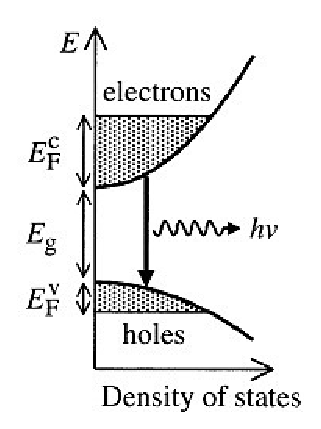
\includegraphics[width=30mm]{57.eps}
    \label{fig:5.7}
  \end{minipage}
 \\ [\intextsep]
Occupancy of the conduction and valence band states in the degenerate limit at $T = 0$. The electrons and holes have separate Fermi energies $E_F^c$ and $E_F^v$ respectively which are determined by the number of carriers injected into the bands. The conduction and valence bands are filled up to their respective Fermi levels, as shown by the shading.}

\subsection{Degeneracy}
At high carrier densities, the classical limit will no longer be valid. The Fermi energies will be positive, and it is essential to use Fermi-Dirac statistics to describe the electron and hole distributions. This situation is called \textbf{degeneracy}.

In the extreme limit of $T = 0$, all the states up to the Fermi energy are filled and all states above it are empty. The Fermi energies can be calculated explicitly (see Exercise 5.10) and are given by:
\begin{equation}\label{equa:5.13}
  E_F^{c,v}=\frac{\hbar^2}{2m_{e,h}^*}(3\pi^2N_{e,h})^{\frac{2}{3}}
\end{equation}
The distribution of the carriers in this limit is shown in Fig. 5.7. Electron-hole recombination can occur between any states in which there is an electron in the upper level and a hole in the lower level. Recombination is thus possible for a range of photon energies between $E_g$ and ($E_g+E_F^c+E_F^v$). We therefore expect to observe a broad emission spectrum starting at $E_g$ up to a sharp cut-off at ($E_g+E_F^c+E_F^v$).

As finite temperatures the carriers will still be degenerate provided that $E_F^{c,v}\gg k_BT$, where $E_F^{c,v}$ is calculated using eqn \ref{equa:5.13}. As $T$ increases, the Fermi-Dirac functions smear out around the Fermi energies, and we expect to observe that the cut-off at ($E_g + E_F^c + E_F$) will be broadened over an energy range $\sim k_BT$.

Figure 5.8 shows the emission spectrum of the III-V alloy semiconductor $\mathrm{Ga_{o.47}In_{0.53}As}$ in the degenerate limit. $\mathrm{Ga_{o.47}In_{0.53}As}$ has a direct gap of 0.81 eV at the lattice temperature $T_L$ of 10 K. The spectra were obtained using the techniques of time-resolved photoluminescence spectroscopy described in Section 5.3.4 below. The figure shows the emission spectrum recorded at two different times after the sample has been excited with an ultrashort ( $<8$ ps) pulse from a dye laser operating at 610 nm. Each pulse has an energy of 6 nJ and is able to excite an initial carrier density of $2\times 10^{24}m^{-3}$.

The spectrum taken 24 ps after the pulse arrives rises sharply at $E_g$, and then shows a flat plateau up to $\sim0.90$ eV. The spectrum then gradually falls off to zero at higher energies. The flat plateau is a signature of the degenerate carriers, while the high energy tail is an indication that the effective carrier temperature is higher than $T_L$ due to the `hot carrier' effect. In this case, the effective carrier temperature is 180 K. At 250 ps the carrier density is lower because a significant number of the electrons and holes have recombined, and the carriers have also cooled to a temperature of 55 K. At still longer times, the spectrum continues to narrow as the carrier density decreases and the carriers cool further towards the lattice temperature of 10 K. Eventually, the carrier density falls to the point where classical statistics are appropriate, and the emission only occurs at energies close to $E_g$. The analysis of this data is explored in more detail in Exercise 5.14.
\subsection{Photoluminescence spectroscopy}
Photoluminescence spectroscopy is mainly used as a diagnostic and development tool in semiconductor research. The usual goal is to develop electroluminescent devices such as light-emitting diodes and lasers. This is usually only achieved after the emission mechanisms have been studied in detail using photoluminescence spectroscopy.

Photoluminescence spectra can be recorded with an experimental arrangement such as the one shown in Fig. 5.9. The sample is mounted in a variable temperature cryostat and is illuminated with a laser or bright lamp with photon energy greater than $E_g$. If a liquid helium cryostat is used, sample temperatures from 2 K upwards are easily obtained. The luminescence is emitted at lower frequencies and in all directions. A portion is collected with a lens and focussed onto the entrance slit of a spectrometer. The spectrum is recorded by scanning the spectrometer and measuring the intensity at each wavelength with a sensitive detector such as a photomultiplier tube. Alternatively, the whole spectrum is recorded at once using an array of detectors such as a charge coupled device (CCD).

A number of useful variations of the basic photoluminescence technique have been developed over the years. In \textbf{photoluminescence excitation spectroscopy} (PLE), the sample is excited with a tunable laser, and the intensity of the luminescence at the peak of the emission is measured as the laser wavelength is tuned. Since the shape of the emission spectrum is independent of the way the carriers are excited, the signal strength is simply proportional to the carrier density, which in turn is determined by the absorption coefficient. (See Exercise 5.6.) Hence the signal is proportional to the absorption coefficient at the laser wavelength. This might seem to be a very complicated way to measure the absorption, but it is actually very useful. Many semiconductor samples are grown as thin layers on top of a thick substrate which is opaque at the wavelengths of interest. This makes it impossible to perform direct transmission measurements, and the use of the PLE technique allows the absorption spectrum to be measured in conditions where it would not be possible otherwise.

In \textbf{time-resolved photoluminescence spectroscopy} the sample is excited with a very short light pulse and the emission spectrum is recorded as a function of time after the pulse arrives. The spectra are obtained using the arrangement shown in Fig. 5.9 but with an ultrafast pulse laser as the excitation source. Lasers emitting pulses shorter than 1 ps are now readily available, and the time resolution is usually limited by the response time of the detector. Time resolutions down to $\sim100$ ps can be obtained using photomultiplier tubes, while resolutions down to 1 ps or better are possible using `streak camera' or `up-conversion' techniques. The time-dependence of the emission spectrum gives direct information about the carrier relaxation and recombination mechanisms, and allows the radiative lifetimes to be measured. Figure 5.8 gives an example of the data that can be obtained using this technique.
\marginnote{
\begin{minipage}{\textwidth}
    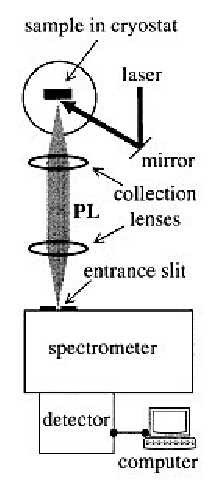
\includegraphics[width=25mm]{59.eps}
    \label{fig:5.9}
  \end{minipage}
 \\ [\intextsep]
Experimental arrangement used for the observation of photoluminescence (PL) spectra. The sample is excited with a laser or lamp with photon energy greater than the band gap. The spectrum is obtained by recording the emission as a function of wavelength using a computer-controlled spectrometer and detector. In photoluminescence excitation spectroscopy (PLE), the detection wavelength is fixed and the excitation wavelength is scanned. In time-resolved photoluminescence spectroscopy, a pulsed laser is used, and the emission at each wavelength is recorded on a fast detector as a function of time after the pulse has arrived.}

\section{Electroluminescence}
Electroluminescence is the process by which luminescence is generated while an electrical current flows through an optoelectronic device. There are two main types of device:
\begin{itemize}
  \item \textbf{light emitting diodes (LEDs)}
  \item \textbf{laser diodes}.
\end{itemize}
We will look at both of these devices in this section, after first discussing the general physical principles which determine their operation.
\subsection{General principles of electroluminescent devices}
Figure 5.10 shows the layer structure and circuit diagram for a typical electroluminescent device. The device consists of several \textbf{epitaxial} layers grown on top of a thick crystal \textbf{substrate}. The epitaxial layers consist of a p-n diode with a thin \textbf{active region} at the junction. The diode is operated in forward bias with a current flowing from the p-layer through to then-layer underneath. The luminescence is generated in the active region by the recombination of electrons that flow in from the n-type layer with holes that flow in from the p-type side.

The microscopic mechanisms that determine the emission spectrum are exactly the same as the ones discussed in the context of photoluminescence in Sections 5.3.1-5.3.3. The only difference is that the carriers are injected electrically rather than optically. At room temperature we therefore expect a single emission line of width $\sim k_BT$ at the band gap energy $E_g$. Hence $E_g$ determines the emission wavelength.

We pointed out in Section 5.2 that the radiative efficiency of indirect gap materials is low. Commercial electroluminescent devices are therefore made from direct gap compounds. Any direct gap semiconductor can, in principle, be used for the active region, but in practice only a few materials are commonly employed. The main factors that determine the choice of the material are:
\begin{enumerate}
  \item the size of the band gap;
  \item constraints relating to lattice matching;
  \item the ease of p-type doping.
\end{enumerate}
The first point is obvious: the band gap determines the emission wavelength. The second and third points are practical ones relating to the way the devices are made. These are discussed further below.

The term \textbf{lattice matching} relates to the relative size of the lattice parameters of the epitaxial layers and the substrate. The thin epitaxial layers are grown on top of a substrate crystal, as shown in Fig. 5.10(a). This is done for practical reasons. It is hard to grow large crystals with sufficient purity to emit light efficiently. We therefore grow thin ultra-pure layers on top of a substrate of poorer optical quality by various techniques of crystal \textbf{epitaxy}. The crystal growth conditions constrain the epitaxial layers to form with the same unit cell size as the substrate crystal. This means that the epitaxial layers will be highly strained unless they have the same lattice constant as the substrate, that is, that we have `lattice matching' between the epitaxial layers and the substrate. If this condition is not satisfied, crystal dislocations are likely to form in the epitaxial layers, which would severely degrade the optical quality.

Figure 5.11 plots the band gap of a number of III-V materials used in electroluminescent devices against their lattice constant. The lattice constants of the commonly used substrate crystal are indicated at the top of the figure. The materials separate into two distinct groups. On the right we have the arsenic and phosphorous compounds which crystallize with the cubic zinc blende structure, while on the left we have the nitride compounds which have the hexagonal wurtzite structure. We will discuss the cubic materials first, and then consider the nitrides afterwards.

For many years, the optoelectronics industry has been mainly based on GaAs. GaAs emits in the infrared at 870 nm, and by mixing it with AlAs to form the alloy $\mathrm{Al_xGa_{1-x}As}$, light emitters for the range 630-870 nm can be produced. (See Example 5.1.) Lattice-matched AlGaAs can easily be grown on GaAs substrates because of the convenient coincidence that the lattice constants of GaAs and AlAs are almost identical. AlGaAs emitters are widely used in local area fibre optic networks operating around 850 nm, and also for red LEDs.

AlGaAs is an example of a `ternary' alloy which contains three elements. `Quaternary' alloys such as $\mathrm{(Al_yGa_{1-y})_xIn_{1-x}P}$ can also be formed. All of these arsenic and phosphorous alloys suffer from the problem that they become indirect as the band gap gets larger. This limits their usefulness to the red and near-infrared spectral range.

Applications in the fibre optics industry require light emitting devices that operate around $\mathrm{1.3\mu m}$ and $\mathrm{1.55\mu m}$. These are the wavelengths where silica fibres have the lowest dispersion and loss respectively. Emitters for these wavelengths tend to be made from the quaternary alloy $\mathrm{Ga_xIn_{1-x}As_yP_{1-y}}$. Lattice matching to InP substrates can be achieved if $x\approx 0.47y$. This allows a whole range of direct gap compounds to be made with emission wavelengths varying from $\mathrm{0.92} \mu m$ to $\mathrm{1.65\mu m}$. See Table 5.1.

Until fairly recently, it has been very difficult to make efficient electroluminescent devices for the green and blue spectral regions using III-V compounds. This is because of the problem that has already been mentioned, namely that the arsenic and phosphorous compounds become indirect as the band gap gets larger. However, in 1995 Shuji Nakamura at Nichia Chemical Industries in Japan made an important breakthrough and reported the successful development of LEDs based on gallium nitride compounds. GaN has a direct band gap of 3.5 eV at 4 K (see Fig. 5.3) and 3.4 eV at room temperature. By alloying it with InN, which has a direct gap of 1.9 eV at 300 K, the emission wavelength can be varied between 360 nm (ultraviolet) and 650 nm (red). This enables the entire visible spectrum to be covered using nitrides for the blue and green colours, and AlGainP alloys for the reds.

It is interesting to consider why it took so long to develop the nitride devices. It was well known that the nitrides would in principle make good blue/green emitters, but no commercial devices were available. The reason for this relates to the third point on our list of factors affecting the choice of electroluminescent materials, namely the difficulty of p-type doping. This is a problem that has also dogged other wide band gap materials. For example, the direct gap II-VI compounds like ZnSe and CdSe should also, in principle, make good LEDs for the blue/green/yellow spectral regions, but they have never found widespread commercial application due to the doping problem.

P-type doping is difficult in wide band gap semiconductors because they have very deep acceptor levels. The energies of the acceptors are given by eqn \ref{equa:7.29} with $m_e^*$ replaced by $m_h^*$. The high value of $m_h^*$ and the relatively small value of $\epsilon_r$ increases the acceptor energies, and hence reduces the number of holes which are thermally excited into the valence band at room temperature. This last point follows from the Boltzmann factor ( eqn \ref{equa:5.11}) with $E$ equal to the acceptor binding energy, which is significantly larger than $k_B T$. The low hole density gives the layers a high resistivity, which causes ohmic heating when the current flows and hence device failure. Nakamura's breakthrough came after discovering new techniques to activate the holes in p-type GaN by annealing the layers in nitrogen at $\mathrm{700^\circ C}$.

In the next chapter we will describe how the use of quantum well layers has led to further developments in the field of electroluminescent materials. In fact, many commercial devices now routinely use quantum wells in the active region. This is especially true in laser diodes, but it is also increasingly so for LEDs as well.
\subsection{Light emitting diodes}
The operating principle of an LED can be understood with reference to the band diagram shown in Fig. 5.12. The p and n regions are both very heavily doped to produce degenerate distributions of holes in the p-region and electrons in the n-region. In thermal equilibrium at zero bias, the Fermi energy must be the same at every point in the device. The bands therefore align with the Fermi energies of the p- and n-regions at the same energy, as shown in Fig. 5.12(a). At the junction, a depletion region is formed, with neither electrons nor holes present. No light can be emitted, because there is no point within the device where there is a significant population of both electrons and holes.

The situation is different when a forward bias of $V_0\sim E_g/e$ is applied to drive a current through the device. This shifts the Fermi levels relative to each other as shown in Fig. 5.12(b). The depletion region shrinks, allowing the electrons in the n-region to diffuse into the p-region, and \textit{vice versa}. This creates a region at the junction where both electrons and holes are present. The electrons recombine with the holes, emitting photons at energy $E_g$ by interband luminescence. The electrons and holes that recombine are replenished by the current flowing through the device from the external circuit, which was given previously in Fig. 5.10(b).
\marginnote{
\begin{minipage}{\textwidth}
    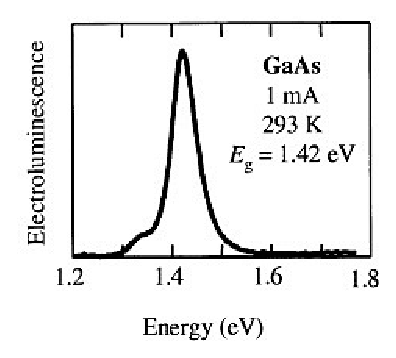
\includegraphics[width=30mm]{513.eps}
    \label{fig:5.13}
  \end{minipage}
 \\ [\intextsep]
Electroluminescence spectrum of a GaAs LED at room temperature. (After A.D. Ashmore, Personal communication)}

Figure 5.13 shows the spectrum of a forward-biased GaAs p-i-n diode with a current of 1 mA flowing through the device. The light is generated in the thin i-region at the junction between the p- and n-regions. As mentioned previously, GaAs has a band gap of 1.42 eV at room temperature, which gives emission in the near-infrared around 870 nm. The full width at half maximum of the emission line is 58 meV, which is about twice $k_BT$ at 293 K.

\subsection{Diode lasers}
Semiconductor lasers are more difficult to make than LEDs, but they give superior performance in terms of their output efficiency, spectral linewidth, beam quality and response speed. They are therefore used for the more demanding applications, leaving the simpler ones for the cheaper LED devices. They are mainly made from GaAs-based materials, and operate in the red and nearinfrared spectral regions. However, blue laser diodes have recently become available following the development of efficient nitride-based emitters.

The acronym `laser' stands for `Light Amplification by Stimulated Emission of Radiation'. As the name suggests, laser operation is based on the quantum mechanical process of \textbf{stimulated emission}. This should be distinguished from the process of \textbf{spontaneous emission} that is responsible for luminescence. (See Section B.1 in Appendix B.) Stimulated emission causes an \textit{increase} in the photon number as the light interacts with the atoms of the medium, which in turn leads to optical amplification. This contrasts with the process of absorption which \textit{reduces} the number of photons, and hence causes attenuation.

Consider the interaction between a light wave of frequency $\nu$ and a medium containing atoms with an electronic transition at energy $h\nu$, as illustrated in Fig. B.2. The absorption processes causes beam attenuation, while stimulated emission causes amplification. The transition rates for the two processes are given by eqns B.5 and B.6 respectively. In the normal conditions of thermal equilibrium, the population of the lower level $N_1$ will be greater than the population of the upper level $N_2$ by the Boltzmann factor given in eqn B.8. This means that the absorption rate exceeds the stimulated emission rate, and there is net beam attenuation. However, if we were somehow to arrange for $N_2$ to be larger than $N_1$, then the reverse would be true. The stimulated emission rate would exceed the absorption rate, and there would be net beam amplification. The condition with $N_2 > N_1$ is called \textbf{population inversion}. It is a necessary condition for laser oscillation to occur.

In Section 5.3.1 we explained how the carrier distributions after injection of electrons and holes are not those of full thermal equilibrium. The top of the valence band is empty of electrons, while the bottom of the conduction band is filled with them. We therefore have population inversion at the band gap frequency $E_g/e$. This gives rise to net optical gain, which can be used to obtain laser operation if an optical cavity is provided.
\marginnote{
\begin{minipage}{\textwidth}
    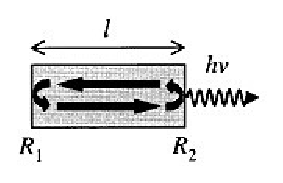
\includegraphics[width=25mm]{514.eps}
    \label{fig:5.14}
  \end{minipage}
 \\ [\intextsep]
Schematic diagram of a laser cavity formed by reflections from the end surfaces of the gain medium of length $l$. The reflectivities of the surfaces are taken to be $R_1$ and $R_2$ respectively, with $R_1\gg R_1$.}

Figure 5 .14 shows a schematic diagram of a laser cavity formed from a gain medium with mirrors at either end. This is the typical arrangement for a semiconductor laser diode, which usually consists of just the semiconductor chip itself. The reftectivities of the semiconductor-air surfaces at the edge of the crystal are typically around $30 \%$. (See Exercise 5.16.) This may be sufficient in itself to obtain lasing, although in what follows we assume that the reflectivities $R_1$ and $R_2$ at the two ends are different, and that $R_1\gg R_2$.

On passing a current through the p-n junction of a laser diode, light at frequency $\nu\approx E_g/h$ is generated by electroluminescence. This light is reflected back and forth within the cavity, and experiences gain due to the population inversion between the conduction and valence bands. At some particular value of the \textbf{injection current} $I_{in}$ called the \textbf{threshold current} $I_{th}$, the laser will begin to oscillate. For current values above $I_{th}$, the light output power of the laser increases linearly with $I_{in}$. This is illustrated in Fig. 5.15(a). The output power is coupled out of the cavity by transmission through the mirror with the lower reflectivity, which is called the \textbf{output coupler} of the laser.

Once the laser is oscillating, the emission spectrum will be determined by the resonant \textbf{longitudinal modes} of the optical cavity. The resonant modes must satisfy the condition that they form standing waves between the mirrors, and hence that there are an integer number of half-wavelengths within the cavity. This condition can be written:
\begin{equation}\label{equa:5.14}
  \text{integer}\times{\frac{\lambda'}{2}}=l
\end{equation}
where $\lambda'$ is the wavelength inside the crystal, which is equal to $\lambda/n$, $\lambda$ being the air wavelength and $n$ the refractive index. This means that the frequencies of the longitudinal modes must satisfy:
\begin{equation}\label{equa:5.15}
  \nu=\text{integer}\times{\frac{c}{2nl}}
\end{equation}
The laser will oscillate at one or several of these resonant frequencies. The best lasers are single longitudinal mode devices, and have emission line widths in the MHz range. This is many orders of magnitude smaller than that of the equivalent LED.

The condition for stable oscillation of the laser is that the light intensity in the cavity should not change with time. This implies that the gain in the laser medium must exactly balance any losses suffered by the light during a roundtrip of the cavity. This condition allows us to work out the value of the gain in the medium when the laser is oscillating.

We assume that there is population inversion inside the medium, and hence that there is optical amplification at the transition frequency $\nu$. We define the incremental gain coefficient $\gamma_{\nu}$ as:
\begin{equation}\label{equa:5.16}
  dI=+\gamma_{\nu}dx\times I(x)
\end{equation}
This is exactly the same definition as for the absorption coefficient in eqn \ref{equa:1.3}, except that the intensity is now growing with distance rather than diminishing. Integration of eqn \ref{equa:5.16} yields:
\begin{equation}\label{equa:5.17}
  I(x)=I_0e^{\gamma_{\nu}x}
\end{equation}
We follow the light at frequency $\nu$ around a round-trip of the cavity shown in Fig. 5.14. In stable laser oscillation, the increase of the intensity due to the gain must exactly balance the losses due to the imperfect reflectivity of the end mirrors and any other losses that may be present in the medium. This condition may be written:
\begin{equation}\label{equa:5.18}
  R_1R_2e^{2\gamma_{\nu}l}e^{-2\alpha_bl}=1
\end{equation}
\marginnote{
\begin{minipage}{\textwidth}
    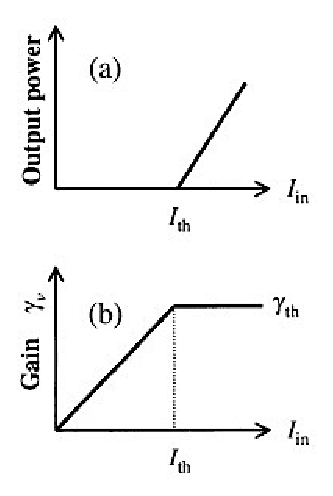
\includegraphics[width=25mm]{515.eps}
    \label{fig:5.15}
  \end{minipage}
 \\ [\intextsep]
(a) Power output and (b) gain coefficient $\gamma_\nu$ as a function of injection current $I_{in}$ in a semiconductor laser diode. $I_{th}$ is the threshold injection current, and $\gamma_{th}$is the threshold gain required for stable laser oscillation.}

The factor of 2 in the two exponentials allows for the fact that the light passes through the gain medium twice during a round trip. The attenuation coefficient $\alpha_b$ in eqn \ref{equa:5.18} accounts for scattering losses and absorption due to processes other than interband transition, for example impurity absorption. The oscillation condition in eqn \ref{equa:5.18} can be re-written:
\begin{equation}\label{equa:5.19}
  \gamma_{th}=\alpha_b-\frac{1}{2l}\ln(R_1R_2)
\end{equation}
This defines the threshold gain $\gamma_{th}$ required to make the laser oscillate. Direct gap semiconductors such as GaAs have very large gain coefficients due to their high density of states and short radiative lifetimes. This makes it possible to overcome the output coupling losses with cavity lengths of order 1 mm or less.

We assume that the gain coefficient increases linearly with the injection current $I_{in}$, as indicated in Fig. 5.15(b). When $I_{in} = I_{th}$, the gain reaches the value $\gamma_{th}$ defined by eqn \ref{equa:5.19}, at which point the laser begins to oscillate. Once the laser is oscillating, the gain must be clamped at the value of $\gamma_{th}$, because otherwise the gain would exceed the losses, and the stability condition set out in eqn \ref{equa:5.18} would not hold. Thus for $I_{in} > I_{th}$, the extra electrons and holes injected into the junction do not produce any more gain, but recombine directly by stimulated emission, and cause the output power to increase, as indicated in Fig. 5.15(a).

The output power $P_{out}$ above threshold can be written:
\begin{equation}\label{equa:5.20}
  P_{out}=\eta\frac{h\nu}{e}(I_{in}-I_{th})
\end{equation}
where $\eta$ is the quantum efficiency. $\eta$ defines the fraction of injected electron-hole pairs that generate laser photons. The quantum efficiency determines the \textbf{slope efficiency} in watts per amp through
\begin{equation}\label{equa:5.21}
  \text{slope efficiency}=\frac{P_{out}}{(I_{in}-I_{th})}=\frac{\eta h\nu}{e}
\end{equation}
In an ideal laser diode we would have $\eta=1$ and the slope efficiency would be equal to the theoretical maximum of $h\nu/e$. Many of the best diode lasers come quite close to this ideal limit.

The main reason why $\eta$ would be less than unity in a real laser diode relates to issues of \textbf{optical confinement} and \textbf{electrical confinement}. The device will not work efficiently unless we c;an arrange that the injection current is confined to the same part of the device where the light is confined. This is not necessarily an easy task due to the inherently planar nature of semiconductor lasers. The devices have very small dimensions (e.g. $\mathrm{1\mu m}$) in the vertical ($z$) direction, and much larger directions (e.g. several hundred microns) in the horizontal $x$, $y$ plane. The light is generated in the thin active region, and is emitted from the edge of the chip. In such a planar structure, the light tends to spread out in the $y$, $z$ plane, while the current tends to spread out in the $x$, $y$ direction. This leads to the possibility that the current and light might not overlap properly in the $x$, $y$ plane, in which case we would have poor quantum efficiency.

There are many different ways to achieve optical and electrical confinement, and we can understand the basic principles by looking at a specific example. Figure 5.16 gives a schematic diagram of an oxide-confined GaAs-AlGaAs heterostructure stripe laser. The `stripe' is defined by the gap in the oxide layers deposited on the top of the device during the fabrication process. The current flows in the -$z$ direction, between the top and bottom metal contacts. The top contact only connects to the p-region in between the insulating oxide layers, and so the current is confined to the long thin rectangular strip of the $x$, $y$ plane defined by the fabrication process.

The light, on the other hand, propagates in the $\pm x$ direction. The shape of the laser mode in the $y$, $z$ plane is determined by \textbf{waveguide} effects. This refers to the confinement of a light beam in the direction perpendicular to its propagation instead of the usual divergence due to diffraction. The confinement in the $z$ direction is achieved through the tendency of the light to propagate in the region with the largest refractive index, which can be understood in terms of repeated total internal reflections at the interfaces between the high and low refractive index materials. This vertical confinement is easily achieved in \textbf{heterojunction} devices such as the one shown in Fig. 5.16. In the example given, the active region is made of GaAs, which has a higher refractive index than the AlGaAs `cladding' layers on either side.

The optical confinement in the y direction is more difficult. It is either achieved by index guiding or gain guiding. Index-guiding is the same effect as that used to produce the vertical confinement. The lateral patterning of the top of the chip can produce small variations in the effective refractive index in the $y$ direction through strain or other effects. Gain guiding, on the other hand, follows as a consequence of current confinement. The semiconductor layers have very strong absorption at the laser wavelength except in the regions where there is gain due to population inversion. Hence the optical mode will be extremely lossy except in the gain regions defined by the current confinement. This is the case with the example shown in Fig. 5.16.

The reader is referred to the references given in the further reading list for more detailed information about the many different types of semiconductor laser that have been made. In the next chapter, we will explain how the use of quantum wells in the active region has led to superior performance and greater flexibility in the emission wavelength.

\section*{Chapter Summary}
\definecolor{shadecolor}{rgb}{1,0.9,0.9}
\begin{shaded}
\begin{itemize}
  \item Luminescence is the generic name for light emission by spontaneous emission in solids. Photoluminescence is the re-emission of light following absorption of higher energy photons. Electroluminescence is the luminescence generated by electrical excitation.
  \item The emission rate is proportional to the matrix element for the transition, the density of states, and the occupancy factors of the upper and lower levels.
  \item Transitions with high absorption coefficients have short radiative lifetimes. Efficient luminescence is only obtained when the radiative lifetime is shorter than the non-radiative lifetime.
  \item Interband luminescence occurs when an electron in the conduction band drops to the valence band with the emission of a photon. The process is equivalent to the recombination of an electron-hole pair. The transition is represented by a downward vertical arrow on the band diagram.
  \item The interband luminescence spectrum if usually independent of the way the material is excited. The emission wavelength corresponds to the fundamental band gap of the material.
  \item Direct gap materials have short radiative lifetimes ($\sim 1 \mathrm{ns}$) and are strong emitters. Indirect gap materials have much longer radiative lifetimes and are generally very inefficient emitters.
  \item The carriers generated by photoexcitation rapidly relax to the bottom of their bands before recombining, and come to a state of quasi-equilibrium with separate Fermi energies for the electrons and holes. The luminescence spectrum can be calculated from the thermal distributions of the carriers.
  \item Light emitting diodes consist of p-n diodes with the light emitting material in the  active region at the junction between the p and n layers. Light is emitted when the diode is forward biased. LEDs are usually made from direct gap semiconductors.
  \item The injection of electrons and holes into the conduction and valence bands can produce population inversion at the band gap frequency. This can support laser operation if the gain due to stimulated emission balances the round trop losses in the optical cavity.
  \item Semiconductor laser are usually planar structures with the light emitted from the edge of the chip. The cavity is formed between the end mirrors at the air-semiconductor interfaces.
\end{itemize}
\end{shaded}

\section*{Further Reading}
A good introductory overview of luminescent processes in solids may be found in Elliott and Gibson (1974). Interband luminescence in semiconductors is discussed in Pankove (1971) and Yu and Cardona (1996). More detailed discussions may be found in Landsberg (1991) or Voos et al. (1980).

An authoritative discussion of time-resolved luminescence spectroscopy may be found in Shah (1999).
The physics of electroluminescence is discussed in most optoelectronics texts, for example Bhattacharya (1997), Chuang (1995), Sze (1981), Sze (1985), or Wilson and Hawkes (1998). The development of nitride light emitters is discussed in Nakamura et al. (2000), while detailed information about semiconductor laser diodes may be found in Silfvast (1996), Svelto (1998) or Yariv (1997).

\chapter{Semiconductor Quantum Wells}\label{chap:6}
\chapter{Free Electrons}\label{chap:7}

\definecolor{shadecolor}{rgb}{0.9,0.9,0.9}
\begin{shaded}
In this chapter we will investigate the optical properties associated with free electrons. As the name suggests, these are electron systems that experience no restoring force from the medium when driven by the electric field of a light wave. The two main solid state systems that exhibit strong free electron effects are:
\begin{itemize}
  \item \textbf{Metals}. Metals contain large densities of free electrons that originate from the valence electrons of the metal atoms.
  \item \textbf{Doped semiconductors}. n-type semiconductors contain free electrons, while p-type materials contain free holes. The free carrier density is determined by the concentration of impurities used for the doping.
\end{itemize}

We will begin our discussion of their optical properties by using the Drude-Lorentz model introduced in Section 2.1.3 of Chapter 2. This will enable us to explain the main optical property of metals that we mentioned in Section 1.4.3, namely that they reflect strongly in the visible spectral region. We will then apply our knowledge of interband transitions from Chapter 3 to obtain a better understanding of the detailed form of the reflectivity spectra of metals such as aluminium and copper. Next we will apply the Drude-Lorentz model to doped semiconductors to explain why doping causes infrared absorption. Finally, we will consider the collective oscillations of the whole free carrier gas. This will naturally lead us to the notion of plasmons, which are elementary excitations of the quantized plasma oscillations.
\end{shaded}

\section{Plasma reflectivity}
A neutral gas of heavy ions and light electrons is called a plasma. Metals and doped semiconductors can be treated as plasmas because they contain equal numbers of fixed positive ions and free electrons. The free electrons experience no restoring forces when they interact with electromagnetic waves. This contrasts with bound electrons that have natural resonant frequencies in the visible or ultraviolet spectral regions due to the restoring forces of the medium.

In this section we will derive a formula for the dielectric constant of an electron plasma using the classical oscillator model discussed in Section 2.2 of Chapter 2. As noted in Section 2.1.3, this approach combines the \textbf{Drude model} of free electron conductivity with the \textbf{Lorentz model} of dipole oscillators, and is therefore known as the \textbf{Drude-Lorentz model}.

We begin by considering the oscillations of a free electron induced by the AC electric field E (t) of an electromagnetic wave. The equation of motion for the displacement $x$ of the electron is:
\begin{equation}\label{equa:7.1}
  m_0\frac{d^2x}{dt^2}+m_0\gamma\frac{dx}{dt}=-e\varepsilon(t)=-e\varepsilon_0e^{-i\omega t}
\end{equation}
where $\omega$ is the frequency of the light, and $\varepsilon_0$ is its amplitude. The first term represents the acceleration of the electron, while the second is the frictional damping force of the medium. The term on the right hand side is the driving force exerted by the light. Equation \ref{equa:7.1} is the same as the equation of motion
for a bound oscillator given in eqn \ref{equa:2.5}, except that there is no restoring force term because we are dealing with free electrons.

By substituting $x = x_0e^{-i\omega t}$ into eqn \ref{equa:7.1}, we obtain
\begin{equation}\label{equa:7.2}
  x(t)=\frac{e\varepsilon(t)}{m_0(\omega^2+i\gamma\omega)}
\end{equation}
The polarization $P$ of the gas is equal to $-Nex$, where $N$ is the number of electrons per unit volume. By recalling the definitions of the electric displacement $D$ and the relative dielectric constant $\epsilon_r$ (cf. eqns A.2 and A.3), we can write:
\begin{eqnarray}
% \nonumber to remove numbering (before each equation)
\nonumber  D &=& \epsilon_r\epsilon_0\varepsilon \\
\nonumber  &=& \epsilon_0\varepsilon+P \\
   &=& \epsilon_0\varepsilon-\frac{Ne^2\varepsilon}{m_0(\omega^2+i\gamma\omega) }  \label{equa:7.3}
\end{eqnarray}
Therefore:
\begin{equation}\label{equa:7.4}
  \epsilon_r(\omega)=1-\frac{Ne^2}{\epsilon_0m_0}\frac{1}{(\omega^2+i\gamma\omega)}
\end{equation}
This equation is identical to eqn \ref{equa:2.14} for the bound oscillator except that the resonant frequency $\omega_0$ is zero and we have not yet considered the effects of background polarizability. Equation \ref{equa:7.4} is frequently written in the more concise form:
\begin{equation}\label{equa:7.5}
  \epsilon_r(\omega)=1-\frac{\omega_p^2}{(\omega^2+i\gamma\omega)}
\end{equation}
where
\begin{equation}\label{equa:7.6}
  \omega_p=\left(\frac{Ne^2}{\epsilon_0m_0}\right)^{\frac{1}{2}}
\end{equation}
$\omega_p$ is known as the \textbf{plasma frequency}.

Let us first consider a lightly damped system. In this case, we put $\gamma = 0$ in eqn \ref{equa:7.5} so that
\begin{equation}\label{equa:7.7}
  \epsilon_r(\omega)=1-\frac{\omega_p^2}{\omega^2}
\end{equation}
The complex refractive index $\tilde{n}$ of the medium is related to the complex dielectric constant by $\tilde{n} = \sqrt{\epsilon_r}$ (cf. eqn \ref{equa:1.19}). This means that $\tilde{n}$ is imaginary for $\omega <\omega_p$ and positive for $\omega > \omega_p$, with a value of zero precisely at $\omega = \omega_p$. The reflectivity $R$ can be calculated from eqn \ref{equa:1.26}:
\begin{equation}\label{equa:7.8}
  R=|\frac{\tilde{n}-1}{\tilde{n}+1}|^2
\end{equation}
By substituting the frequency dependence of $\tilde{n}$ into this formula, we see that $R$ is unity for $\omega\le\omega_p$, and then decreases for $\omega\ge\omega_p$, approaching zero at $\omega=\infty$. This frequency dependence is plotted in Fig. 7.1.

The basic conclusion is that we expect the reflectivity of a gas of free electrons to be $100 \%$ for frequencies up to $\omega_p$. This result is very well confirmed by experimental data. In Sections 7.3 and 7.4 below we will see how the plasma reflectivity effect is observed in both metals and doped semiconductors.

\section{Free carrier conductivity}
In deriving eqn \ref{equa:7.7}, we neglected the damping of the free carrier oscillations. We can recast the equation of motion in a way that makes the physical significance of the damping term more apparent. To do this we note that $\dot{x}$ is the electron velocity $\mathbf{v}$. Hence we can rewrite eqn \ref{equa:7.1} as:
\begin{equation}\label{equa:7.9}
  m_0\frac{d\mathbf{v}}{dt}+m_0\gamma\mathbf{v}=-e\bm{\varepsilon}
\end{equation}
Since $m_0\mathbf{v}$ is the momentum $\mathbf{p}$, we see that:
\begin{equation}\label{equa:7.10}
  \frac{d\mathbf{p}}{dt}=-\frac{\mathbf{p}}{\tau}-e\bm{\varepsilon}
\end{equation}
where we have replaced the damping rate $\gamma$ by the reciprocal of the damping time $\tau$. This shows that the electron is being accelerated by the field, but loses its momentum in time $\tau$. In other words, r is the \textbf{momentum scattering time}.

In an AC field of the form $\varepsilon(t) = \varepsilon_0e^{-i\omega t}$, we look for solutions to the equation of motion with $x = x_0e^{-i\omega t}$. This implies that $|\mathbf{v}|= \dot{x}$ also has a time variation of the form $\mathbf{v} = \mathbf{v}_0e^{-i\omega t}$. On substituting this into eqn \ref{equa:7.9}, we obtain:
\begin{equation}\label{equa:7.11}
  \mathbf{v}(t)=\frac{-e\tau}{m_0}\frac{1}{1-i\omega t}\boldsymbol{\varepsilon}(t)
\end{equation}
The current density $\mathbf{j}$ is related to the velocity and field through:
\begin{equation}\label{equa:7.12}
  \mathbf{j}=-Ne\mathbf{v}=\sigma\boldsymbol{\varepsilon}
\end{equation}
where $\sigma$ is the electrical conductivity. On combining eqns \ref{equa:7.11} and \ref{equa:7.12}, we obtain the \textbf{AC conductivity} $\sigma(\omega)$:
\begin{equation}\label{equa:7.13}
  \sigma(\omega)=\frac{\sigma_0}{1-i\omega\tau}
\end{equation}
where
\begin{equation}\label{equa:7.14}
  \sigma_0=\frac{Ne^2\tau}{m_0}
\end{equation}
$\sigma_0$ is the conductivity measured with DC electric fields.

In principle, the momentum scattering time can be deduced from eqn \ref{equa:7.13} by measuring the conductivity of the free carrier gas as a function of frequency. However, for a metal or doped semiconductor, the value of $\tau$ is typically in the range $10^{-14}-10^{-13}$ s. This means that we have to go to near optical frequencies to notice any departure from the DC conductivity. Hence we must use optical measurements to obtain information about $\tau$.

By comparing eqns \ref{equa:7.4} and \ref{equa:7.13}, we see that the AC conductivity and the dielectric constant are related to each other through:
\begin{equation}\label{equa:7.15}
  \epsilon_r(\omega)=1+\frac{i\sigma(\omega)}{\epsilon_0\omega}
\end{equation}
Thus optical measurements of $\epsilon_r(\omega)$ are equivalent to AC conductivity measurements of $\sigma(\omega)$.

At very low frequencies that satisfy $\omega\ll\tau^{-1}$, we can derive a useful relationship between the conductivity of the free carrier gas and the attenuation coefficient for electromagnetic waves. This can be achieved by first splitting $\epsilon_r(\omega)$ into its real and imaginary components in accordance with eqn \ref{equa:1.18}. Equation \ref{equa:7.5} with $\gamma=\tau^{-1}$ gives:
\begin{eqnarray}
% \nonumber to remove numbering (before each equation)
  \epsilon_1 &=& 1-\frac{\omega_p^2\tau^2}{1+\omega^2\tau^2} \label{equa:7.16} \\
  \epsilon_2 &=& \frac{\omega_p^2\tau^2}{\omega(1+\omega^2\tau^2)} \label{equa:7.17}
\end{eqnarray}
We then work out $n$ and $\kappa$, the real and imaginary parts of the complex refractive index, using eqns \ref{equa:1.22} and \ref{equa:1.23}, and hence deduce the attenuation coefficient $\alpha$ from $\kappa$. Since $\omega\tau\ll 1$ implies that $\epsilon_2\gg\epsilon_1$, we can obtain solutions with $n\approx\kappa=(\epsilon_2/2)^{1/2}$. Using eqn \ref{equa:1.16} we therefore obtain:
\begin{equation}\label{equa:7.18}
  \alpha=\frac{2\omega(\epsilon_2/2)^{\frac{1}{2}}}{c}=\left(\frac{2\omega_p^2\tau\omega}{c^2}\right)^{\frac{1}{2}}
\end{equation}
We can put this equation in a more accessible form by noting from eqn \ref{equa:7.14} that $\omega_p^2\tau=\sigma_0/\epsilon_0$ and from eqn A.28 that $c^2=1/{\epsilon_0\mu_0}$. This gives:
\begin{equation}\label{equa:7.19}
  \alpha=(2\sigma_0\omega\mu_0)^{\frac{1}{2}}
\end{equation}
Hence we see that the attenuation coefficient is proportional to the square root of the DC conductivity and the frequency.

Equation \ref{equa:7.19} implies that AC electric fields can only penetrate a short distance into a conductor such as a metal. This well-known phenomenon is called the \textbf{skin effect}. If the field strength varies as $\exp(-z/\delta)$ with the distance $z$ from the surface, then the power falls off as $\exp(-2z/\delta)$. By comparison with the definition of $\alpha$ in eqn \ref{equa:1.4}, we see that:
\begin{equation}\label{equa:7.20}
  \delta=\frac{2}{\alpha}=(\frac{2}{\sigma_0\omega\mu_0})
\end{equation}
$\delta$ is known as the \textbf{skin depth}.

At higher frequencies the relationship given in eqn \ref{equa:7.19} breaks down because the approximation $\omega\tau\ll 1$ is no longer valid. In this case we can derive a different frequency dependence for the attenuation coefficient. This will be discussed when we consider the absorption due to free carriers in doped semiconductors in Section 7.4.1

\section{Metals}
The free electron model of metals was proposed by P. Drude in 1900. The model provides a basic explanation for why metals are good conductors of heat and electricity, and is the starting point for more sophisticated theories. As we will see here, it is also successful in explaining a number of important optical properties, such as the fact that metals tend to be good reflectors. On the other hand, we will need to use band theory to explain the details of the optical spectra, and also to account for the coloured appearance of some metals, for example, copper and gold.

\subsection{The Drude model}
The Drude free electron model of metals considers the valence electrons of the atoms to be free. When an electric field is applied, the free electrons accelerate and then undergo collisions with the characteristic scattering time $\tau$ introduced in eqn \ref{equa:7.10}. The electrical conductivity is therefore limited by the scattering, and measurements of $\sigma$ allow the value of $\tau$ to be determined through eqn \ref{equa:7.14}.

The free electron density $N$ in the Drude model is equal to the density of metal atoms multiplied by their valency. Table \ref{tab:7.1} lists the Drude free electron densities for a number of common metals. The values of $N$ are in the range $10^{28}-10^{29} \mathrm{m}^{-3}$. These very large free electron densities explain why metals have high electrical and thermal conductivities. The plasma frequencies calculated using eqn \ref{equa:7.6} are also tabulated in Table \ref{tab:7.1}, together with the wavelength $\lambda_p$ that corresponds $\omega_p$. It is apparent that the very large values of $N$ lead to plasma frequencies in the ultraviolet spectral region.

In the visible spectral region where $\omega/2\pi\sim10^{15}$ Hz, we are usually in a situation with $\omega\gg\gamma$. This is because $\tau=\gamma^{-1}$ is typically of order $10^{-14}$ s. Therefore the simplification of eqn \ref{equa:7.5} to eqn \ref{equa:7.7} is a good approximation. With $\omega_p$ in the ultraviolet, the visible photons have frequencies below $\omega_p$ and thus $\epsilon_r$ is negative. As discussed in Section 7.1, this means that the reflectivity is expected to be $100\%$ up to $\omega_p$. This explains the first and most obvious optical property of metals, namely that they tend to be good reflectors at visible frequencies.

\begin{table}
%\caption{Free electron density and plasma properties of some metals. The figures are for room temperature unless stated otherwise. The electron densities are based on data taken from reference [1]. The plasma frequency $\omega_p$ is calculated from eqn \ref{equa:7.6}, and $\lambda_p$ is the wavelength corresponding to this frequency.}\label{tab:7.1}
  \begin{tabular}{lcccc}

     % after \\:   or \cline{col1-col2} \cline{col3-col4} ...
     Metal & Valency & N & $\omega_p/2\pi$ & $\lambda_p$ \\
       &  & $(10^{28}m^{-3})$ & $(10^{15}Hz)$ & (nm) \\
     Li(77K) & 1 & 4.70 & 1.95 & 154 \\
     Na(5K) & 1 & 2.65 & 1.46 & 205 \\
     K(5K) & 1 & 1.40 & 1.06 & 282 \\
     Rb(5K) & 1 & 1.15 & 0.96 & 312 \\
     Cs(5K) & 1 & 0.91 & 0.86 & 350 \\
     Cu & 1 & 8.47 & 2.61 & 115 \\
     Ag & 1 & 5.86 & 2.17 & 138 \\
     Au & 1 & 5.90 & 2.18 & 138 \\
     Be & 2 & 24.7 & 4.46 & 67 \\
     Mg & 2 & 8.61 & 2.63 & 114 \\
     Ca & 2 & 4.61 & 1.93 & 156 \\
     Al & 3 & 18.1 & 3.82 & 79 \\

   \end{tabular}
\end{table}

A striking implication of the free carrier model is that the dielectric constant changes from being negative to positive as we go through the plasma frequency. This means that the reflectivity ceases to be $100\%$ above $\omega_p$ (see Fig. 7.1) and some of the light can be transmitted through the metal. Thus we expect that all metals will eventually become transmitting if we go far enough into the ultraviolet so that $\omega>\omega_p$. This phenomenon is known as the \textbf{ultraviolet transparency of metals}.

In order to observe the ultraviolet transmission threshold at  the plasma frequency, it is necessary that there should be no other absorption processes occurring at $\omega_p$. This condition is best satisfied in the alkali metals. Table 7.2 lists the wavelengths of the ultraviolet transmission edges observed in the alkalis. The experimental wavelengths can be compared with those predicted from the calculated plasma frequency tabulated in Table \ref{tab:7.1}. The experimental results are in reasonable agreement with the predictions, and show the correct trend on descending the periodic table. The discrepancies can be explained to a large extent by replacing the free electron mass with the electron effective mass derived from the band structure of the metal. (See Exercise 7.4.)

Figure 7.2 shows the measured reflectivity of aluminium as a function of photon energy from the infrared to the ultraviolet spectral region. We see that the reflectivity is over $80\%$ up to $\sim15$ eV, and then drops off to zero at higher frequencies. Thus aluminium shows the characteristic ultraviolet transparency edge predicted by the Drude model. The relatively featureless reflectivity at visible frequencies is exploited in commercial mirrors.

The plasma frequency listed in Table \ref{tab:7.l} corresponds to a photon energy of 15.8 eV. The dotted line in Fig. 7.2 gives the reflectivity predicted from eqn \ref{equa:7.7} with $\hbar\omega_p = 15.8$ eV. On comparing the experimental and theoretical results, we see that the model accounts for the general shape of the spectrum, but there are some important details that are not explained.

An improved attempt to model the experimental data can be made by computing the dielectric constant with the damping term included using eqn \ref{equa:7.5}. Example \ref{equa:3.3} explains how this is done. The reflectivity calculated for the value of $\tau$ deduced from the DC conductivity, namely $8.0 \times10^{-15}$ s, is plotted as the dashed line in Fig. 7.2. The main difference between the two calculated curves is that the damping causes the reflectivity to be less than unity below $\omega_p$, and the ultraviolet transmission edge is slightly broadened. However, this is only a relatively small effect because $\omega_p\gg\tau^{-1}$.

The inclusion of damping makes a small improvement in the fit to the data, but there are two important features that are still not explained. Firstly, the reflectivity is significantly lower than predicted, and secondly, there is a dip around 1.5 eV, where we would have expected a featureless curve. Both of these points can be explained by considering the interband absorption rates. These are discussed in the next section.

\subsection{Inter band transitions in metals}
The absorption of light by direct interband transitions was discussed in detail in Chapter \ref{chap:3}. Direct transitions involve the promotion of electrons to a higher band by absorption of a photon with the correct energy. The electron does not change its $k$ vector significantly because of the very small momentum of the photon. Thus the transitions appear as vertical arrows on the $E-k$ band diagram of the solid.

Interband absorption is important in metals because the electromagnetic waves penetrate a short distance into the surface, and if there is a significant probability for interband absorption, the reflectivity will be reduced from the free carrier value. The interband absorption spectra of metals are determined by their complicated band structures and Fermi surfaces. Furthermore, we need to consider transitions at frequencies in which the free carrier properties are also important. For this reason we will only consider two examples to illustrate the general principles, namely aluminium and copper, and then make some general comments about other metals such as silver and gold.

\textbf{Aluminium}

The band diagram of aluminium is shown in Fig. 7.3. Aluminium has an electronic configuration of $[\mathtt{Ne}]3s^23p^1$ with three valence electrons. The crystal structure is face-centred cubic, which has a body-centred cubic (bee) reciprocal lattice, as shown in Fig. C.5 of Appendix C. The first Brillouin zone is completely full, and the valence electrons spread into the second, third and slightly into the fourth zones. The band structure appears quite complex due to the irregular shape of the bee Brillouin zone. However, the bands are actually very close to the free electron model, with significant departures only in the vicinity of the Brillouin zone boundaries. The bands are filled up to the Fermi energy $E_p$, which is marked on the diagram. Direct transitions can take place from any of the states below the Fermi level to unoccupied bands directly above them on the $E-k$ diagram.

Fermi's golden rule given in eqn \ref{equa:3.2} tells us that the absorption rate is proportional to the density of states for the transition. The dip in the reflectivity at 1.5 eV which is apparent in Fig. 7.2 is a consequence of the `parallelband' effect. This occurs when there is a band above the Fermi level that is approximately parallel to another band below $E_F$. In this case, the interband transitions from a large number of occupied $k$ states below the Fermi level will all occur at the same energy. Hence the density of states at the energy difference between the two parallel bands will be very high, which will result in a particularly strong absorption at this photon energy.

Inspection of the band diagram of aluminium shows that the parallel-band effect occurs at both the W- and K-points of the Brillouin zone. These transitions have been identified on Fig. 7.3. The energy separation of the parallel bands is approximately 1.5 eV in both cases. The enhanced transition rate at this photon energy thus explains the reflectivity dip observed at 1.5 eV in the experimental data. Moreover, we can see from the band diagram that there will be further transitions between bands below the Fermi level to unoccupied bands above $E_F$ at a whole range of photon energies greater than 1.5 eV. The density of states for these transitions will be lower than at 1.5 eV because the bands are not parallel. However, the absorption rate is still significant, and accounts for the reduction of the reflectivity to a value below that predicted by the Drude model in the visible and ultraviolet spectral regions.

\textbf{Copper}
\marginnote{
\begin{minipage}{\textwidth}
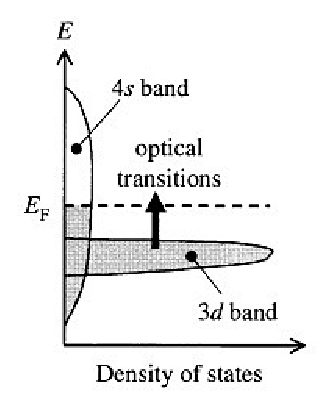
\includegraphics[width=20mm]{74.eps}\label{fig:7.4}\\[\intextsep]
Schematic density of states for the $3d$ and $4s$ bands of a transition metal such as copper.
\end{minipage}}

Copper has an electronic configuration of $[\mathtt{Ar}]3d^{10}4s^1$. The outer $4s$ bands approximate reasonably well to free electron states with a dispersion given by $E = \hbar^2k^2 /2m_0$. They therefore form a broad band covering a wide range of energies. The $3d$ bands, on the other hand, are more tightly bound and are relatively dispersionless, occupying only a narrow range of energies. The density of states for the two bands is illustrated schematically in Fig. 7.4. The narrow $3d$ bands can hold ten electrons, and therefore their density of states is sharply peaked. The $4s$ band, which can hold two electrons, is much broader, with a smaller maximum. The 11 valence electrons of copper fill up the $3d$ band, and half fill the $4s$ band. The Fermi energy therefore lies within the $4s$ band above the $3d$ band. Interband transitions are possible from the filled $3d$ bands to unoccupied states in the $4s$ band above $E_F$, as illustrated in Fig. 7.4. This implies that there will be a well-defined threshold for interband transitions from the $3d$ bands to the $4s$ band.

Figure 7.5 shows the actual band structure and density of states of copper. The general features indicated in Fig. 7.4 are apparent in the calculated curves. The $3d$ electrons lie in relatively narrow bands with very high densities of states, while the $4s$ bands are much broader with a lower density of states. The Fermi energy lies in the middle of the $4s$ band above the $3d$ band. Interband transitions are possible from the $3d$ bands below $E_F$ to unoccupied levels in the $4s$ band above $E_F$. The lowest energy transitions are marked on the band diagram in Fig. 7.5. The transition energy is 2.2 eV which corresponds to a wavelength of 560 nm.

Figure 7.6 shows the measured reflectivity of copper from the infrared to the ultraviolet spectral region. Based on the plasma frequency given in Table \ref{tab:7.1}, we would expect near-$100\%$ reflectivity for photon energies below 10.8 eV, which corresponds to an ultraviolet wavelength of 115 nm. However, the experimental reflectivity falls off sharply above 2 eV due to the interband absorption edge discussed above. This explains why copper has a reddish colour.

\textbf{Silver and gold}

The arguments used for copper can be applied to the other noble metals. The important parameter is the energy gap between the d-bands and the Fermi energy, as shown in Fig. 7.4. In gold the interband absorption threshold occurs at a slightly higher energy than copper, which explains why it has a yellowish colour. In silver, on the other hand, the interband absorption edge is around 4 eV. This frequency is in the ultraviolet, and so the reflectivity remains high throughout the whole visible spectrum. (See Fig. 1.5.) This explains why silver does not have any particular colour, and also why it is so widely used for making mirrors. Gold is also be used for mirrors, but only at infrared wavelengths.

\section{Doped semiconductors}
The controlled doping of semiconductors with impurities is an essential part of solid state technology. The general principles are discussed in Section C.1 of Appendix C. The atoms of the pure crystal have four valence electrons. The introduction of \textbf{donor} impurities from group V of the periodic table provides an excess of electrons, while \textbf{acceptor} impurities from group III lead to a deficit of electrons, which is equivalent to an excess of holes. Doping that produces excess electrons is called \textbf{n-type}, while doping that produces excess holes is called \textbf{p-type}.

Experimental measurements on doped semiconductors show that the presence of impurities give rise to new absorption mechanisms and also to a free carrier plasma reflectivity edge. Our aim here is to explain these effects by applying a suitably modified version of the free carrier model and by considering the quantized levels created by the impurity atoms. In the two subsections that follow, we will first consider the free carrier effects, and then move on to discuss the absorption associated with the impurity levels.
\subsection{Free carrier reflectivity and absorption}

The free electron model developed in Sections 7.1 and 7.2 can be applied to doped semiconductors if we make two appropriate modifications. Firstly, we must account for the fact that the electrons and holes are moving in the conduction or valence band of a semiconductor. This is easily achieved by assuming that the carriers behave as particles with an effective mass $m^*$ rather than the free electron mass $m_0$. Secondly, we must remember that there are other mechanisms that can contribute to the dielectric constant as well as the free carrier effects. The main extra effect that we will need to consider is the contribution to the polarization due to the optical response of the bound electrons.

The two modifications mentioned above can be handled if we rewrite eqn \ref{equa:7.3} in the following form:
\begin{eqnarray}
% \nonumber to remove numbering (before each equation)
\nonumber  D &=& \epsilon_r\epsilon_0\varepsilon  \\
\nonumber   &=& \epsilon_0\varepsilon+P_{other}+P_{free carrier} \\
   &=& \epsilon_{opt}\epsilon_0\varepsilon-\frac{Ne^2\varepsilon}{m^*(\omega^2+i\gamma\omega)} \label{equa:7.21}
\end{eqnarray}
The term $P_{other}$ accounts for the polarizability of the bound electrons, while the effective mass $m^*$ accounts for the band structure of the semiconductor. The carrier density $N$ that appears in this equation is the density of free electrons or holes generated by the doping process. Note that the sign of the charge cancels, and so the only difference between electrons and holes in this treatment is in the effective mass that is used.

The free carrier effects due to doping are most noticeable in the spectral region $5-30\um$, where we would normally expect the semiconductor to be completely transparent. Hence the value of $\epsilon_{opt}$ that we use in eqn \ref{equa:7.21} is the one measured in the transparent spectral region below the interband absorption edge. This value is known from the refractive index of the undoped semiconductor: $\epsilon_{opt} = n^2$. (See eqn \ref{equa:1.24} with $\kappa = 0$ below the band edge.)

Equation \ref{equa:7.21} tells us that the frequency dependence of the dielectric constant is given by:
\begin{equation}\label{equa:7.22}
  \epsilon_r(\omega)=\epsilon_{opt}-\frac{Ne^2}{m^*\epsilon_0}\frac{1}{(\omega^2+i\gamma\omega)}
\end{equation}
This can be rewritten as:
\begin{equation}\label{equa:7.23}
  \epsilon_r(\omega)=\epsilon_{opt}\left(1-\frac{\omega_p^2}{(\omega^2+i\gamma\omega)}\right)
\end{equation}
where the plasma frequency $\omega_p$ is now given by
\begin{equation}\label{equa:7.24}
  \omega_p^2=\frac{Ne^2}{\epsilon_{opt}\epsilon_0m^*}
\end{equation}
We have written the dielectric constant in this way to make the link to the Drude model apparent. The difference between the plasma frequency for the semiconductor given in eqn \ref{equa:7.24} and that given in eqn \ref{equa:7.6} is that we have replaced $m_0$ by $m^*$, and we have included a non-resonant dielectric constant to account for the background polarizability of the bound electrons.

If we assume that the system is lightly damped, then we can ignore the damping term in eqn \ref{equa:7.23}. This then implies that $\epsilon_r$ is negative below $\omega_p$ and positive at higher frequencies. We thus expect to observe a plasma reflectivity edge at $\omega_p$ just as we did in metals. Since the carrier density is much smaller than in metals, the plasma edge occurs at frequencies in the infrared spectral range. This prediction is very well borne out by infrared reflectivity data.

Figure 7.7 shows the measured reflectivity of n-type InSb as a function of the electron density. The fundamental absorption edge at the band gap of InSb occurs at $6\um$, while the phonon absorption band lies around $50\um$. Thus we would expect pure InSb to be transparent in the wavelength range shown and have a featureless reflectivity spectrum. Instead, the data shows a well-defined reflectivity edge, which shifts to shorter wavelengths as the electron density increases, in accordance with eqn \ref{equa:7.24}.

One very striking feature of the data is the zero in the reflectivity at wavelengths just below the plasma edge. This occurs at a frequency given by (see Exercise 7.8):
\begin{equation}\label{equa:7.25}
  \omega^2=\frac{\epsilon_{opt}}{\epsilon_{opt}-1}\omega_p^2
\end{equation}
By fitting this formula to the data, the effective mass of InSb can be determined. (See Exercise 7.9.)

At frequencies above $\omega_p$, the presence of free carriers leads to the absorption of light. This effect is called \textbf{free carrier absorption}, and can be observed in the near-infrared spectral region below the fundamental absorption edge at the band gap, where the semiconductor would normally be transparent. To see how this effect arises, we split the dielectric constant given in eqn \ref{equa:7.23} into its real and imaginary parts. This gives:
\begin{eqnarray}
% \nonumber to remove numbering (before each equation)
  \epsilon_1 &=& \left(1-\frac{\omega_p^2\tau^2}{1+\omega^2\tau^2}\right)\label{equa:7.26} \\
  \epsilon_2 &=& \frac{\epsilon_{opt}\omega_p^2\tau}{\omega(1+\omega^2\tau^2)} \label{equa:7.27}
\end{eqnarray}
where we have made the usual substitution of $\tau^{-1}$ for $\gamma$. In a typical semiconductor, with $\tau\sim10^{-13}$ s at room temperature, it is safe to make the approximation  $\omega\tau\gg1$ at frequencies in the near-infrared. Furthermore, the free carrier term in $\epsilon_r$ will be small. Therefore we can assume $\epsilon_1\approx\epsilon_{opt}$. and that $\epsilon_2\ll\epsilon_1$. In these conditions we find solutions to eqns \ref{equa:1.22} and \ref{equa:1.23} with $n=\sqrt{\epsilon_{opt}}$ and $\kappa = \epsilon_2/2n$. This allows us to deduce the absorption coefficient using eqn \ref{equa:1.16}. The result is:
\begin{equation}\label{equa:7.28}
  \alpha_{free carrier}=\frac{\epsilon_{opt}\omega_p^2}{nc\omega^2\tau}=\frac{Ne^2}{m^*\epsilon_0nc\tau}\frac{1}{\omega^2}
\end{equation}
This shows that the free carrier absorption is proportional to the carrier density and should vary with frequency as $\omega^{-2}$.

Experimental data on a number of n-doped samples leads to the conclusion that $\alpha_{free carrier}\propto\omega^{-\beta}$, where $\beta$ is in the range $2-3$. The departure of $\beta$ from the predicted value of 2 is caused by the failure of our assumption that $\tau$ is independent of $\omega$. To see why this is important, we illustrate the physical processes that are occurring during free carrier absorption in Fig. 7.8. The figure shows the conduction band of an n-type semiconductor, which is filled up to the Fermi level determined by the free carrier density. Absorption of a photon excites an electron from an occupied state below the Fermi level to an unoccupied level above $E_F$. The photon only has a very small momentum compared to the electron, and therefore cannot change the electron's momentum significantly. It is obvious from Fig. 7.8 that a scattering event must occur to conserve momentum in the process. Hence the absorption must be proportional to the scattering rate $1/\tau$, in accordance with the prediction of eqn \ref{equa:7.28}.

The mechanisms that can contribute to the momentum conserving process in free carrier absorption include phonon scattering and scattering from the ionized impurities left behind by the release of the free electrons from their dopants. It is a sweeping oversimplification to characterize all the possible scattering processes with a single frequency-independent scattering time $\tau$ deduced from the DC conductivity. Thus it is hardly surprising that the experimental data does not exactly show an $\omega^{-2}$ dependence.

The free carrier reflectivity and absorption of p-type semiconductors can be modelled by a similar treatment to the one developed here for n-type samples. The only change that has to be made is in the effective mass that is used in the calculation. Thus we would expect that all the main results will hold, provided we take account of the fact that the scattering time for holes is not necessarily the same as that for electrons. However, p-type samples also show another effect in addition to those related with the free carriers, which is discussed below.

Figure 7.9 shows the valence band of a p-type III-V semiconductor. This is a larger scale version of the band structure diagram given previously in Fig. 3.5, except that now there are unfilled states near $k = 0$ due to the p-type doping. Optical transitions can take place in which an electron is promoted from an occupied state below $E_F$ in the light hole (lh) band to an empty one in the heavy hole (hh) band above $E_F$. This is called \textbf{intervalence band absorption}. Other intervalence band transitions are possible in which an electron is promoted from the split-off (SO) band to either the lh or hh band. The range of energies over which these transitions occur can be calculated from the effective masses, the doping density and the split-off band energy (see Exercise 7.12). The absorption occurs in the infrared, and can be a strong process because no scattering events are required to conserve momentum.

\subsection{Impurity absorption}
The n-type doping of a semiconductor with donor atoms introduces a series of hydrogenic levels just below the conduction band. These quantized states are called \textbf{donor levels}, and are illustrated schematically in Fig. 7.10. The impurity levels gives rise to two new absorption mechanisms, in addition to any of the free carrier effects discussed in the previous section. If the donor states are occupied, it will be possible to absorb photons by exciting electrons between the levels as illustrated in Fig. 7.10(a). On the other hand, if the states are empty, then it will be possible to absorb light by exciting electrons from the valence band to the donor states as illustrated in Fig. 7.10(b).

We consider first the transitions between the donor levels illustrated in Fig. 7.10(a). For such a process to occur, the donor levels must be occupied. This will be the case at low temperatures, when there is insufficient thermal energy to promote the electrons from the donor levels into the  conduction band.

The frequencies of the donor level transitions can be calculated if the energies of the impurity states are known. In the simplest model, we assume that the electron is released into the crystal, and is then attracted back towards the positively charged impurity atom. The electron and the ionized impurity then form a hydrogenic system bound together by their mutual Coulomb attraction. As a first approximation, we can use the Bohr formula, provided we use the effective mass $m^*$ instead of the free electron mass $m_0$, and also include the dielectric constant $\epsilon_r$ for the semiconductor. Hence the energy of the donor levels $E_{\texttt{n}}^D$ will be given by:
\begin{equation}\label{equa:7.29}
  E_{\texttt{n}}^D=-\frac{m_e^*}{m_0}\frac{1}{\epsilon_r^2}\frac{R_H}{\texttt{n}^2}
\end{equation}
where $R_H$ is the hydrogen Rydberg (13.6 eV) and $\texttt{n}$ is an integer.

At low temperatures we can assume that all the electrons from the donors will be in the ground state $\texttt{n} = 1$ impurity level. Optical transitions can then take place in which the electrons are promoted to higher donor levels or into the conduction band by absorption of a photon. Figure 7.10(a) illustrates two possible transitions of this type, in which the electron is promoted to either the $\texttt{n} = 2$ or the $\texttt{n} = 3$ donor level. These transitions give rise to absorption lines analogous to the hydrogen Lyman series with frequencies given by:
\begin{equation}\label{equa:7.30}
  h\nu=\frac{m_e^*}{m_0}\frac{R_H}{\epsilon_r^2}\left(1-\frac{1}{\texttt{n}^2}\right)
\end{equation}
where $\texttt{n}$ is the quantum number of the final impurity level. If we insert typical values into eqn \ref{equa:7.30} we find that the photon energies are in the range 0.01- 0.1 eV. This means that the transitions occur in the infrared spectral region.

Figure 7.11 shows the absorption spectrum of n-type silicon at liquid helium temperatures. The sample was doped with phosphorous at a density of $1.2\times 10^{20} \mathrm{m^{-3}}$. The absorption lines correspond to transitions exciting electrons from the $\texttt{n} = 1$ shell to higher shells. In the language of atomic physics, these are $ls\rightarrow\texttt{n}p$ transitions. These transitions converge at high $\texttt{n}$ to the donor ionization energy of phosphorous in silicon, which is 45 meV.

The spectrum shown in Fig. 7.11 is actually more complicated than eqn \ref{equa:7.30} would suggest. It actually consists of two series of transitions, which are labelled as either $\texttt{n}p_0$ or $\texttt{n}p_{\pm}$. The $\texttt{n}p_0$ series obey eqn \ref{equa:7.30} very well, but the $\texttt{n}p_{\pm}$ transitions have a different frequency dependence. This complexity is caused by the anisotropy of the effective mass of silicon. The frequency dependence of the two series can be modelled by assigning different effective Rydbergs for the `O' and `$\pm$' states. (See Exercise 7.13.)

We now consider briefly the absorption mechanism shown in Fig. 7.10(b). These transitions can be observed at temperatures when the donor levels are partly unoccupied due to the thermal excitation of the electrons into the conduction band. Absorption processes can then occur in which electrons are excited from the top of the valence band to the empty donor levels.

The valence band $\rightarrow$ donor level transitions occur at photon energies just below the band gap $E_g$, with a threshold given by $E_g - E_1^D$. However, the transitions tend to be broadened into a continuum both by the thermal effects and by the fact that transitions can take place from a whole range of states within the valence band. Hence the impurity transitions cause a smearing of the abrupt absorption edge at the band gap found in pure semiconductors. The absorption strength will always be weak compared to the interband and excitonic transitions due to the relatively small number of impurity atoms compared to the density of states within the conduction band. On the other hand, the transitions occur in the spectral region just below the band gap where we would normally expect no absorption at all. Hence these transitions do have an effect on the fundamental absorption edge, and make precise determinations of $E_g$ from the absorption spectra at room temperature more difficult.

We have restricted our attention here exclusively to n-type semiconductors for the sake of simplicity. The same effects can of course occur in p-type materials.

\section{Plasmons}
Equation \ref{equa:7.7} tells us that the dielectric constant of a lightly damped gas of free electrons is expected to be zero at $\omega_p$. This suggests that something unusual might happen at this frequency. This is indeed the case, as we discuss here.

A plasma system such as a metal consists of a fixed lattice of positive ions together with a gas of free electrons which exactly cancels the charge of the ions. Figure 7.12(a) illustrates a slab of the ions and electrons from within the bulk of the crystal. Consider a displacement of the whole free electron gas as illustrated in Fig. 7.12(b). The fixed lattice of positive ions will exert a restoring force to oppose this displacement of the electrons. This may cause the electrons to overshoot as shown in Fig. 7.12(c), which would then cause a restoring force in the opposite direction. The net result is that the whole electron gas can oscillate backwards and forwards with respect to the fixed lattice of positive ions. These oscillations are called \textbf{plasma oscillations}.

The frequency of the plasma oscillations can be calculated as follows. The displacement of the electrons by $\pm u$ illustrated in Figs. 7.12(b) and (c) gives rise to surface charges at either side of the slab. The surface charge per unit area is $-Neu$, where $N$ is the number of electrons per unit volume in the metal. The unbalanced ions give an identical positive surface charge at the other end of the slab. Gauss's law tells us that the electric field $\varepsilon$ is equal to $Neu/\epsilon_0$. The direction of this electric field is such as to oppose the displacement of the  electrons. The equation of motion for a unit volume of the electron gas is thus:
\begin{equation}\label{equa:7.31}
  Nm_0\frac{d^2u}{dt^2}=-Ne\varepsilon=-\left(\frac{N^2e^2}{\epsilon_0}\right)u
\end{equation}
This can be recast in the more familiar form:
\begin{equation}\label{equa:7.32}
  \frac{d^2u}{dt^2}+\left(\frac{Ne^2}{\epsilon_0m_0}\right)u=0
\end{equation}
This describes the harmonic oscillations of the gas at an angular frequency given by ($Ne^2/\epsilon_0m_0)^{1/2}$, that is, at the plasma frequency $\omega_p$ defined in eqn \ref{equa:7.6}.

This simple analysis confirms that the plasma has a natural resonant frequency at $\omega_p$. The polarization $P$ (i.e. the dipole moment per unit volume) is equal to $Neu$ and is in the opposite direction to the field. Hence the electric displacement $D = \epsilon_0\varepsilon + P$ is zero, which implies that the dielectric constant $\epsilon_r$ is zero. Thus the plasma oscillations correspond to oscillations in the conditions where $\epsilon_r= 0$.

Quantized plasma oscillations are called \textbf{plasmons}. These can be observed in metals by electron energy loss spectroscopy. A beam of electrons with energy $E_{in}\sim2 keV$ is fired at a thin sample. The electrons can excite plasmons as they pass through the metal. The energy $E_{out}$ of the transmitted electrons
will therefore be given by:
\begin{equation}\label{equa:7.33}
  E_{out}=E_{in}-\texttt{n}\hbar\omega_p
\end{equation}
where $\texttt{n}$ is the number of plasmons emitted during the passage through the sample. Thus by measuring the energy of the electrons emerging, the plasma frequency can be determined.

Plasmons can also be observed directly in doped semiconductors. Since the plasma frequencies are much lower, it is possible to use Raman scattering techniques to measure the plasmon energies. The general principles of Raman scattering will be discussed in Section 10.5. The basic point is that the photon energy changes as it traverses the sample through inelastic light scattering processes with the plasmons in the medium. Conservation of energy requires that the energy $\hbar\omega_{out}$ of the outgoing photon must satisfy:
\begin{equation}\label{equa:7.34}
  \hbar\omega_{out}=\hbar\omega_{in}\pm\hbar\omega_p
\end{equation}
where $\hbar\omega_{in}$ is the energy of the incoming photon. The $+$ sign corresponds to plasmon absorption and the $-$ sign to plasmon emission.

Figure 7.13 shows the results of a Raman scattering experiment on n-type GaAs at 300 K. The doping density was $1.75\times10^{23}\mathrm{m^{-3}}$ . The data is plotted as a function of the frequency shift of the light in wave number units. The data shows two clear peaks shifted by $\mathrm{pm}130\mathrm{cm}^{-1}$ relative to the incoming laser beam due to plasmon emission and absorption. The electron effective mass of GaAs is $0.067m_0$ and $\epsilon_{opt}$ is 10.6. Hence from eqn \ref{equa:7.24} we find $\omega_p=2.8\times10^{13}$ Hz, which is equivalent to $150\mathrm{cm}^{-1}$. The experimental data is thus in reasonably good agreement with the model.

\section*{Chapter Summary}
\definecolor{shadecolor}{rgb}{1,0.9,0.9}
\begin{shaded}
\begin{itemize}
  \item Free electron effect are observed in metals and doped semiconductors. They can be modelled by the classical dipole oscillator model with no restoring force term. This approach is called the Drude-Lorentz model.
  \item The free electron plasma reflects strongly up to a specific frequency called the plasma frequency, which depends on the electron density. The damping rate of the oscillations is determined by the momentum scattering time deduced from electrical conductivity measurements.
  \item Metals reflect strongly due to the plasma  reflectivity effect. At frequencies above the plasma frequency, the metals become transparent. This effect is called the ultraviolet transparency of metals.
  \item Interband transitions are possible in metals from states below the Fermi energy to empty levels above it. The interband absorption can reduce the reflectivity from the value predicted by the Drude-Lorentz model, and must therefore be considered to obtain a good fit to experimental reflectivity data.
  \item Doped semiconductors reflect at frequencies in teh infrared due to the plasma reflectivity of the free electrons and holes generated by the doping process. Free carrier absorption effects can be observed at frequencies above the plasma frequency but below the fundamental absoption edge at the band gap.
  \item P-type semiconductors show an additional absorption mechanism in the infrared due to intervalence band transitions.
  \item Doped semiconductors show sharp infrared absorption lines due to impurity transitions at low temperatures. At room temperature, the impurity states broaden the fundamental absorption edge.
  \item Longitudinal plasma oscillations occur at the plasma frequency. The quantized oscillations  are called plasmons. These can be observed by electron energy loss spectroscopy in metals, or by Raman scattering in doped semiconductors.
\end{itemize}
\end{shaded}

\section*{Further Reading}
The properties of electromagnetic waves in a conducting medium are covered in many electromagnetism and optics textbooks, for example Bleaney and Bleaney (1976), Born and Wolf (l 999) or Hecht (1998).

The free carrier model of metals is covered in Singleton (2001). It is also covered in Ashcroft and Mermin (1976), Burns (1985) or Kittel (1996). Kittel gives a good discussion of plasmons in metals.

Free carrier reflectivity and absorption in semiconductors has been reviewed by Pidgeon (1980), and is also covered by Yu and Cardona (1996). Yu and Cardona give further details about intervalence band and impurity absorption.
\chapter{Molecular Materials}\label{chap:8}
\chapter{Luminescence Centres}\label{chap:9}
\chapter{Phonons}\label{chap:10}
\definecolor{shadecolor}{rgb}{0.9,0.9,0.9}
\begin{shaded}
In this chapter we will tum our attention to the interaction between light and the phonons in a solid. Phonons are vibrations of the atoms in a crystal lattice, and have resonant frequencies in the infrared spectral region. This contrasts with the optical properties of bound electrons, which occur at visible and ultraviolet frequencies.

The main optical properties of phonons can be explained to a large extent by classical models. We will therefore make extensive use of the classical dipole oscillator model developed in Chapter \ref{chap:2}. This will allow us to understand why polar solids reflect and absorb light strongly within a band of infrared frequencies. We will then introduce the concepts of polaritons and polarons, before moving on to discuss the physics of inelastic light scattering. We will see how Raman and Brillouin scattering techniques give us complementary information to infrared reflectivity data, which is why they are so extensively used in phonon physics. Finally we will briefly discuss why phonons have a finite lifetime, and how this affects the reflectivity and inelastic scattering spectra.

We will assume that the reader is familiar with the basic physics of phonons, which is covered in all introductory solid state physics texts. A partial list of suitable preparatory reading is given under Further Reading at the end of the chapter.
\end{shaded}

\section{Infrared active phonons}

The atoms in a solid are bound to their equilibrium positions by the forces that hold the crystal together. When the atoms are displaced from their equilibrium positions, they experience restoring forces, and vibrate at characteristic frequencies.

These vibrational frequencies are determined by the phonon modes of the crystal. The resonant frequencies of the phonons occur in the infrared spectral region, and the modes that interact directly with light are called \textbf{infrared active} (IR active). Detailed selection rules for deciding which phonon modes are IR active can be derived by using group theory. At this level we just discuss the general rules based on the dispersion of the modes, their polarization, and the nature of the bonding in the crystal.

The phonon modes of a crystal are subdivided into two general categories:
\begin{itemize}
  \item acoustic or optical;
  \item transverse or longitudinal.
\end{itemize}
It will come as no surprise to realize that it is the `optical' rather than the acoustic modes that are directly IR active. These optically active phonons are able to absorb light at their resonant frequency. The basic process by which a photon is absorbed by the lattice and a phonon is created is represented in Fig. 10.1. Conservation laws require that the photon and the phonon must have the same energy and momentum. We will see below that this condition can only be satisfied for the optical modes.
\marginnote{
\begin{minipage}{\textwidth}
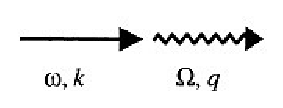
\includegraphics[width=20mm]{101.eps}\label{fig:10.1}\\[\intextsep]
Lattice absorption process by an infrared active phonon. The straight arrow represents the photon that is absorbed, while the wiggly arrow represent the phonon that is created.
\end{minipage}}

\begin{figure}
  \centering
  % Requires \usepackage{graphicx}
  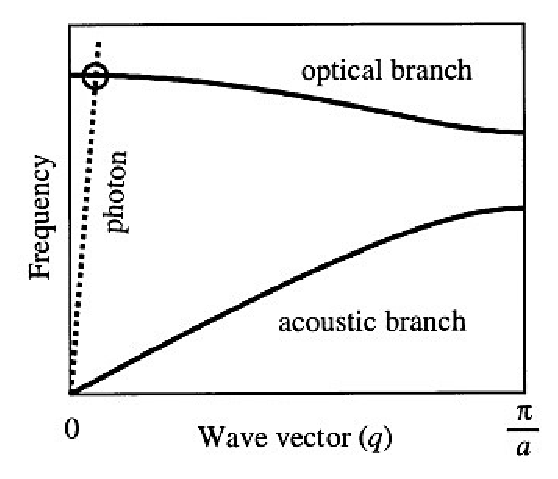
\includegraphics[width=0.5\textwidth]{102.eps}\label{fig:10.2}\\
\end{figure}
\marginnote{Dispersion curves for the acoustic and optical phonon branches in a typical crystal with a lattice constant of a. The dispersion of the photon modes in the crystal is shown by the dotted line.}

Figure 10.2 shows the generic dispersion curves for the acoustic and optical phonons in a simple crystal. The angular frequency $\Omega$ of the acoustic and optical phonons is plotted against the wave vector $q$ in the positive half of the first Brillouin zone. At small wave vectors the slope of the acoustic branch is equal to $\nu_s$, the velocity of sound in the medium, while the optical modes are essentially dispersionless near $q = 0$.

The figure also shows the dispersion of the light waves in the crystal, which have a constant slope of $v = c / n$, where $n$ is the refractive index. The refractive index has been highly exaggerated here in order to make the dispersion of the photon noticeable on the same scale as the phonon dispersion. The requirement that the photon and phonon should have the same frequency and wave vector is satisfied when the dispersion curves intersect. Since $c/n\gg v_s$, the only intersection point for the acoustic branch occurs at the origin, which corresponds to the response of the crystal to a static electric field. The situation is different for the optical branch: there is an intersection at finite $\omega$, which is identified with the circle in Fig. 10.2. Since the optical branch is essentially flat for small $q$, the frequency of this resonance is equal to the frequency of the optical mode at $q = 0$.

Electromagnetic waves are transverse, and can only apply driving forces to the transverse vibrations of the crystal. Therefore they can only couple to the transverse optic (TO) phonon modes. This does not mean that we can now completely forget about the longitudinal optic (LO) phonons. As we will see in Section 10.2.2, the LO modes do in fact play an important role in the infrared properties of crystals.

Photons couple to phonons through the driving force exerted on the atoms by the AC electric field of the light wave. This can only happen if the atoms are charged. Therefore, if the atoms are neutral, there will be no coupling to the light. This means that the crystal must have some ionic character in order for its TO phonons to be optically active.

The ionicity of a solid arises from the way the crystal binding occurs. An ionic crystal consists of an alternating sequence of positive and negative ions held together by their mutual Coulomb attraction. Covalent crystals, by contrast, consist of neutral atoms with the electrons shared equally between the neighbouring nuclei. This means that none of the optical phonons of purely covalent solids like silicon are IR active. Most other materials fall somewhere between these two limits. For example, the bond in a III-V semiconductor is only partly covalent, and the shared electrons lie slightly closer to the group V atoms than to the group III atoms, which gives the bond a partly ionic character.The bonds with an ionic character are called \textbf{polar} bonds to stress the point that the asymmetric electron cloud between the atoms creates a dipole that can interact with electric fields. Provided the bond has some polar character, its phonons can be IR active.

The conclusions of this section are summarized in Table \ref{tab:10.1}.

\begin{table}
  \centering
  %\caption{Infrared activity of the phonon modes in polar and nonpolar crystals. LA: longitudinal acoustic, TA: transverse acoustic, LO: longitudinal optic, TA: transverse optic.}\label{tab:10.1}
  \begin{tabular}{ccc}

     % after \\:   or \cline{col1-col2} \cline{col3-col4} ...
     Mode & Polar & Non-polar \\
     * & crystal & crystal \\
     LA & no & no \\
     TA & no & no \\
     LO & no & no \\
     TO & yes & no \\

   \end{tabular}
\end{table}


\section{Infrared Reflectivity and absorption in Polar Solids}

Experimental data show that polar solids absorb and reflect light very strongly in the infrared spectral region when the frequency is close to resonance with the TO phonon modes. We have come across several examples of this already. For example, the transmission spectra of sapphire and CdSe given in Fig. \ref{fig:1.4} show that there are spectral regions in the infrared where no light is transmitted. This is a consequence of lattice absorption.

The aim of this section is to account for this result by modelling the interaction of photons with TO phonons. To do this we will make extensive use of the classical oscillator model developed in Chapter \ref{chap:2}, especially Section 2.2. This will allow us to calculate the frequency dependence of the complex dielectric constant $\epsilon_r(\omega)$, from which we will be able to determine the important optical properties such as the reflectivity and absorption.

\subsection{The classical oscillator model}

The interaction between electromagnetic waves and a TO phonon in an ionic crystal is most easily treated by considering a linear chain, as illustrated in Fig. \ref{fig:10.3}. The chain consists of a series of unit cells, each containing a positive ion (black circle) and a negative ion (grey circle). The waves are taken to be propagating along the chain in the $z$ direction. We are dealing with a transverse mode, and so the displacement of the atoms is in the $x$ or $y$ directions. Furthermore, in an optic mode the different atoms within each unit cell move  in opposite directions, with a fixed ratio between their displacements which is not necessarily equal to unity.

We are interested in the interaction between a TO phonon mode with $q\approx0$ and an infrared light wave of the same frequency and wave vector. This means that we are considering phonons with a very long wavelength of $\sim\mathrm{10\mu m}$ matched to that of an infrared photon. This phonon wavelength is huge compared to the size of a unit cell in a crystal, which is usually less than $\mathrm{10^{-9}m}$. The size of the atoms has been highly exaggerated in Fig. \ref{fig:10.3} to make the physics of the interaction clearer. In fact, the real size of the atoms is tiny compared to the wavelength, and there will be thousands of unit cells within one period of the wave.

The solid line in the figure represents the spatial dependence of the AC electric field of the infrared light wave. At resonance, the wave vector of the photon and the phonon are the same. This means that the driving force exerted by the light on the positive and negative ions is in phase with the lattice vibration. At the same time, the antiparallel displacements of the oppositely charged atoms generate an AC electric field in phase with the external light. This implies that there is a strong interaction between the TO phonon mode and the light wave when the wave vectors and frequencies match.

For long wavelength TO modes with $q\approx0$, the motion of the atoms in different unit cells is almost identical, and we therefore need to concentrate on what is happening within the unit cell itself. This enables us to see that there is a close connection between the TO phonons at $q = 0$ and the vibrational modes of the molecules from which the crystal is formed. We can therefore make use of some of the principles developed in molecular physics, for example: the selection rules for deciding whether a particular phonon mode is IR or Raman active. (cf. Section 10.5.2.)

The interaction between the TO phonon and the light wave can be modelled by writing down the equations of motion for the displaced ions. The displacements of the positive and negative ions in a TO mode are in opposite directions and are given the symbols $x_+$ and $x_-$ respectively, as indicated in Fig. \ref{fig:10.3}. The appropriate equations of motion are:
\begin{eqnarray}
% \nonumber to remove numbering (before each equation)
  m+\frac{d^2x_+}{dt^2} &=& -K(x_+-x_-)+\texttt{q}\varepsilon(t) \label{equa:10.1} \\
  m-\frac{d^2x_-}{dt^2} &=& -K(x_--x_+)+\texttt{q}\varepsilon(t) \label{equa:10.2}
\end{eqnarray}
where $m_+$ and $m_-$ are the masses of the two ions, $K$ is the restoring constant of the medium, and $\varepsilon(t)$ is the external electric field due to the light wave. The effective charge per ion is taken to be $\pm q$.

By dividing eqn \ref{equa:10.1} by $m_+$ and eqn \ref{equa:10.2} by $m_-$, and then subtracting, we obtain:
\begin{equation}\label{equa:10.3}
  \frac{d^2}{dt^2}(x_+-x_-)=-\frac{K}{\mu}(x_+-x_-)+\frac{\texttt{q}}{\mu}\varepsilon(t)
\end{equation}
where $\mu$ is the reduced mass given by
\begin{equation}\label{equa:10.4}
  \frac{1}{\mu}=\frac{1}{m_+}+\frac{1}{m_-}
\end{equation}
By putting $x = x_+ - x_-$ for the relative displacement of the positive and negative ions within their unit cell, we can recast eqn \ref{equa:10.3} in the simpler form:
\begin{equation}\label{equa:10.5}
  \frac{d^2x}{dt^2}+\Omega_{TO}^2x=\frac{\texttt{q}}{\mu}\varepsilon(t)
\end{equation}
where we have written $\Omega_{TO}^2$ for $K/\mu$. $\Omega_{TO}$ represents the natural vibrational frequency of the TO mode at $q = 0$ in the absence of the external light field.

Equation \ref{equa:10.5} represents the equation of motion for undamped oscillations of the lattice driven by the forces exerted by the AC electric field of the light wave. In reality, we should have incorporated a damping term to account for the finite lifetime of the phonon modes. The physical significance of the phonon lifetime will be discussed further in Section 10.6. At this stage, we simply introduce a phenomenological damping rate $\gamma$, and rewrite eqn \ref{equa:10.5} as
\begin{equation}\label{equa:10.6}
  \frac{d^2x}{dt^2}+\gamma\frac{dx}{dt}+\Omega_{TO}^2x=\frac{\texttt{q}}{\mu}\varepsilon(t)
\end{equation}
This now represents the response of a damped TO phonon mode to a resonant light wave.

Equation \ref{equa:10.6} is identical in form to eqn \ref{equa:2.5} in Chapter \ref{chap:2}, with $m_0$ replaced by $\mu$, $\omega_0$ by $\Omega_{TO}$ and $-e$ by $\texttt{q}$. Therefore, we can use all the results derived in Section 2.2 to model the response of the medium to a light field of angular frequency $\omega$ with $\varepsilon(t) = \varepsilon_0e^{i\omega t}$. In particular, we can go directly to the formula for the frequency dependence of the dielectric constant without repeating all the steps in the derivation. By adapting the symbols appropriately in eqn \ref{equa:2.14}, we immediately write down:
\begin{equation}\label{equa:10.7}
  \epsilon_r(\omega)=1+\chi+\frac{N\texttt{q}^2}{\epsilon_0\mu}\frac{1}{(\Omega_{TO}^2)-\omega^2-i\gamma\omega}
\end{equation}
where $\epsilon_r(\omega)$ is the complex dielectric constant at angular frequency $\omega$. $\chi$ represents the non-resonant susceptibility of the medium, and $N$ is the number of unit cells per unit volume.

Equation \ref{equa:10.7} can be tidied up by introducing the static and high frequency dielectric constants $\epsilon_{st}$ and $\epsilon_{\infty}$ respectively. In the limits of low and high frequency, we obtain from eqn \ref{equa:10.7}:
\begin{equation}\label{equa:10.8}
  \epsilon_{st}\equiv\epsilon_r(0)=1+\chi+\frac{N\texttt{q}^2}{\epsilon_0\mu\Omega_{TO}^2}
\end{equation}
and
\begin{equation}\label{equa:10.9}
  \epsilon_\infty\equiv\epsilon_r(\infty)=1+\chi
\end{equation}
Thus we can write:
\begin{equation}\label{equa:10.10}
  \epsilon_r(\omega)=\epsilon_{\infty}+(\epsilon_{st}-\epsilon_{\infty})\frac{\Omega_{TO}^2}{(\Omega_{TO}^2-\omega^2-i\gamma\omega)}
\end{equation}
This is our main result, which will be used in the next subsections to derive the infrared optical coefficients. As discussed in Section 2.2.2, and in particular in connection with Fig. \ref{fig:2.6}, we should understand `$\omega=\infty$' in a relative sense here. $\epsilon_{\infty}$ represents the dielectric constant at frequencies well above the phonon resonance, but below the next natural frequency of the crystal due, for example, to the bound electronic transitions in the visible/ultraviolet spectral region.

\subsection{The Lyddane-Sachs-Teller relationship}

Before working out the frequency dependence of the infrared reflectivity, it is useful to investigate one rather striking implication of eqn \ref{equa:10.10}. Suppose we have a lightly damped system so that we can set $\gamma=0$. Then at a certain frequency which we label $\omega'$, eqn \ref{equa:10.10} tells us that the dielectric constant can fall to zero. The condition for this to happen is:
\begin{equation}\label{equa:10.11}
  \epsilon_r(\omega')=0=\epsilon_{\infty}+(\epsilon_{st}-\epsilon_{\infty})\frac{\Omega_{TO}^2}{(\Omega_{TO}^2-\omega'^2)}
\end{equation}
This can be solved to obtain:
\begin{equation}\label{equa:10.12}
  \omega'=(\frac{\epsilon_{st}}{\epsilon_{\infty}})^{\frac{1}{2}}\Omega_{TO}
\end{equation}

What does $\epsilon_r=0$ mean physically? In a medium with no free charges, the total charge density will be zero. Hence Gauss's law (eqn A.10) tells us that
\begin{equation}\label{equa:10.13}
  \nabla\cdot\mathbf{D}=\nabla\cdot(\epsilon_r\epsilon_0\boldsymbol{\varepsilon})=0
\end{equation}
where we have made use of eqn A.3 to relate the electric displacement $\mathbf{D}$ to the electric field $\boldsymbol{\varepsilon}$ in a dielectric medium. When we consider the propagation of electromagnetic waves through the dielectric, we look for wave solutions of the form:
\begin{equation}\label{equa:10.14}
  \boldsymbol{\varepsilon}(\mathbf{r},t)=\boldsymbol{\varepsilon}_0e^{i(\mathbf{k}\cdot\mathbf{r}-\omega t)}
\end{equation}
On substituting eqn \ref{equa:10.14} into eqn \ref{equa:10.13}, we usually assume that $\epsilon_r\neq0$ and therefore conclude that $\mathbf{k}\cdot\boldsymbol{\varepsilon}=0$. This tells us that the electric field must be perpendicular to the direction of the wave and therefore that the waves are transverse. However, if $\epsilon_r=0$, we can satisfy eqn \ref{equa:10.13} with waves in which $\mathbf{k}\cdot\boldsymbol{\varepsilon}\neq0$, that is, with longitudinal waves. Thus we conclude that the dielectric can support longitudinal electric field waves at frequencies which satisfy $\epsilon_r(omega)=0$.

In the same way that TO phonon modes generate a transverse electric field wave, the LO phonon modes generate a longitudinal electric field wave. Thus the waves at $\omega=\omega'$ correspond to LO phonon waves, and we identify $\omega'$ with the frequency of the LO mode at $q=0$, namely $\Omega_{LO}$. This allows us to rewrite eqn \ref{equa:10.12} in the following form:
\begin{equation}\label{equa:10.15}
  \frac{\Omega_{LO}^2}{\Omega_{TO}^2}=\frac{\epsilon_{st}}{\epsilon_{\infty}}
\end{equation}
This result is known as the \textbf{Lyddane-Sachs-Teller (LST) relationship}. The validity of the relationship can be checked by comparing the values of $\Omega_{LO}/\Omega_{TO}$ deduced from neutron or Raman scattering experiments with those calculated from eqn \ref{equa:10.15} using known values of the dielectric constants. Some results are given in Table \ref{tab:10.2}. It is apparent that the agreement is generally very good.

\begin{table}
  \centering
  %\caption{Comparison of the measured ratio $\Omega_{LO}/\Omega_{TO}$ for several materials to the value predicted by the Lyddane-Sachs-Teller relationship.}\label{tab:10.2}
  \begin{tabular}{lll}

    % after \\:   or \cline{col1-col2} \cline{col3-col4} ...
    Crystal & $\Omega_{LO}/\Omega_{TO}$ & $(\epsilon_{st}/\epsilon_{\infty})^{\frac{1}{2}}$ \\
    Si & 1 & 1 \\
    GaAs & 1.07 & 1.08 \\
    AlAs & 1.12 & 1.11 \\
    BN & 1.24 & 1.26 \\
    ZnSe & 1.19 & 1.19 \\
    MgO & 1.81 & 1.83 \\
    AgF & 1.88 & 1.88 \\

  \end{tabular}
\end{table}

An interesting corollary of the LST relationship is that it implies that the LO phonon and TO phonon modes of non-polar crystals are degenerate. This follows because there is no infrared resonance, and therefore $\epsilon_{st}=\epsilon_{\infty}$. This is indeed the case for the purely covalent crystals of the group IV elements, namely diamond (C), silicon and germanium.

\subsection{Restrahlen}

Having discussed the properties of the system at the special frequency of $\omega=\Omega_{LO}$. we can now calculate the infrared optical constants. It is easier to understand the general behaviour if we assume that the damping term is small. We thus set $\gamma=0$ in eqn \ref{equa:10.10}, and discuss the properties of a material with a dielectric constant that has the following frequency dependence:
\begin{equation}\label{equa:10.16}
  \epsilon_r(\nu)=\epsilon_{\infty}+(\epsilon_{st}-\epsilon_{\infty})\frac{\nu_{TO}^2}{(\nu_{TO}^2-\nu^2)}
\end{equation}
We have divided all the angular frequencies by $2\pi$ here, so that we can compare the predictions to experimental data, which are usually presented against frequency ($\nu$) rather than angular frequency ($\omega$). We will discuss the effect of including the damping term when we compare our model to the experimental data in connection with Fig. \ref{fig:10.5}.

Figure 10.4(a) plots the frequency dependence of the dielectric constant $\epsilon_r(\nu)$ calculated from eqn \ref{equa:10.16} for a polar crystal with the following parameters: $\nu_{TO} = 10$ THz, $\nu_{LO} = 11$ THz, $\epsilon_{st}=12.1$ and $\epsilon_\infty=10$. These figures are quite close to those that would be found in a typical III-V semiconductor. Note that the phonon frequencies have been chosen to satisfy the LST relationship given in eqn \ref{equa:10.15}.

At low frequencies the dielectric constant is just equal to $\epsilon_{st}$. As $\nu$ increases from 0, $\epsilon_r{\nu}$ gradually increases until it diverges when the resonance at $\nu_{TO}$ is reached. Between $\nu_{TO}$ and $\nu_{LO}$, $\epsilon_r$ is negative. Precisely at $\nu = \nu_{LO}$, $\epsilon_r=0$. Thereafter, $\epsilon_r$ is positive, and gradually increases asymptotically towards the value of $\epsilon_{\infty}$

The most important optical property of a polar solid in the infrared spectral region is the reflectivity. This can be calculated from the dielectric constant using eqn \ref{equa:1.26}:
\begin{equation}\label{equa:10.17}
  R=|\frac{\tilde{n}-1}{\tilde{n}+1}|^2=|\frac{\sqrt{\epsilon_r}-1}{\sqrt{\epsilon_r+1}}|^2
\end{equation}
Figure 10.4(b) plots the reflectivity calculated using eqn \ref{equa:10.17} for the dielectric constant shown in Fig. 10.4(a). At low frequencies the reflectivity is $(\sqrt{\epsilon_{st}}-1)^2/(\sqrt{\epsilon_{st}}+1)^2$. As $\nu$ approaches $\nu_{TO}$, $R$ increases towards unity. In the frequency region between $\nu_{TO}$ and $\nu_{LO}$, $\sqrt{\epsilon_r}$ is imaginary, so that $R$ remains equal to unity. $R$ drops rapidly to zero as $\nu$ increases above $\nu_{LO}$ (see Exercise 10.2), and then increases gradually towards the high frequency asymptote of $(\sqrt{\epsilon_{\infty}}-1)^2/(\sqrt{\epsilon_{\infty}}+1)^2$.

We see from this analysis that the reflectivity is equal to $100\%$ in the frequency region between $\nu_{TO}$ and $\nu_{LO}$. This frequency region is called the \textbf{restrahlen} band. Restrahlen is the German word for `residual rays'. Light cannot propagate into the medium in the restrahlen band.

Figure \ref{fig:10.5} shows experimental data for the reflectivity of InAs and GaAs in the infrared spectral region. InAs has TO and LO phonon frequencies at $218.9cm^{-1}$ and $243.3cm^{-1}$ respectively, while for GaAs we have $\nu_{TO} = 273.3cm^{-1}$ and $\nu_{LO}=297.3cm^{-1}$. We see that the reflectivity is very high for frequencies between the TO and LO phonon frequencies in both materials, and there is a sharp dip in the reflectivity just above the LO phonon resonance.

On comparing these results with the prediction shown in Fig. 10.4(b), we see that the general agreement between the model and the experimental data is very good. The main difference is that in both materials the maximum reflectivity in the restrahlen band is less than $100\%$. This reduction in the reflectivity is caused by ignoring the damping term. (See Example 10.l and Exercise 10.4.) The damping also broadens the edge so that there is only a minimum in $R$ just above $\nu_{LO}$ rather than a zero.

The magnitude of $\gamma$ can be found by fitting the experimental data to the full dependence given in eqn \ref{equa:10.10}. The values of $\gamma$ obtained in this way are around $10^{11}-10^{12}\mathrm{s^{-1}}$, which implies that the optical phonons have a lifetime of about 1-10 ps. The physical significance of this short lifetime will be discussed in Section 10.6.

\subsection{Lattice absorption}
When we introduced the classical oscillator model in Section 2.2 of Chapter \ref{chap:2}, we made the point that we expect high absorption coefficients whenever the frequency matches the natural resonances of the medium. The reader might therefore be wondering why we have been concentrating on calculating the reflectivity rather than the absorption due to the TO phonon resonances.

This question is further prompted by recalling the analogy between the infrared absorption of polar solids and that of isolated molecules. In both cases we are basically treating the interaction of photons with quantized vibrational modes. In molecular physics we usually discuss this in terms of the infrared absorption spectrum. The absorption spectra show strong peaks whenever the frequency coincides with the infrared active vibrational modes and the molecule can absorb a photon by creating one vibrational quantum.This is directly analogous to the process for solids shown in Fig. \ref{fig:10.1} in which a photon is absorbed and a phonon is created.

The answer to these questions is that the lattice does indeed absorb very strongly whenever the photon is close to resonance with the TO phonon. As stressed in Chapter \ref{chap:2}, the fundamental optical properties of a dielectric - the absorption, refraction and reflectivity - are all related to each other because they are all determined by the complex dielectric constant. The distinction between absorption and reflection is merely a practical one. Polar solids have such high absorption coefficients in the infrared that unless the crystal is less than $\sim1\um$ thick, no light at all will be transmitted. This is clearly seen in the transmission spectra of $\mathrm{Al_2O_3}$ and CdSe shown in Fig. \ref{fig:1.4}. For this reason, it is only sensible to consider lattice absorption in thin film samples. In thick crystals, we must use reflectivity measurements to determine the vibrational frequencies. This contrasts with molecular physics, where we are usually dealing with low density gases, which give rise to much smaller absorption coefficients.

The absorption coefficients expected at the resonance with the TO phonon can be calculated from the imaginary part of the dielectric constant. At $\omega=\Omega_{TO}$ we have from eqn \ref{equa:10.10}:
\begin{equation}\label{equa:10.18}
  \epsilon_r(\Omega_{TO})=\epsilon_{\infty}+i(\epsilon_{st}-\epsilon_{\infty})\frac{\Omega_{TO}}{\gamma}
\end{equation}
The extinction coefficient $\kappa$ can be worked out from $\epsilon_r$ using eqn \ref{equa:1.23}, and then the absorption coefficient $\alpha$ can be determined from $\kappa$ using eqn \ref{equa:1.16}. Typical values for $\alpha$ are in the range $10^6-10^7\mathrm{m^{-1}}$. (See Example 10.1 and Exercise 10.6.) This is why the sample must be thinner than $\sim1\um$ in order to perform practical absorption measurements. Infrared absorption measurements on thin film samples do indeed confirm that the absorption is very high at the TO phonon resonance frequency.

\section{Polaritons}
The dispersion curves of the photons and TO phonons were discussed in broad terms in connection with Fig. \ref{fig:10.2}. We now wish to consider the circled intersection point in Fig. \ref{fig:10.2} in more detail. As we will see, the two dispersion curves do not actually cross each other. This is a consequence of the strong coupling between the TO phonons and the photons when their frequencies and wave vectors match. This leads to the characteristic anticrossing behaviour which is observed in many coupled systems.

The coupled phonon-photon waves are called \textbf{polaritons}. As the name suggests, these classical waves are mixed modes which have characteristics of both polarization waves (the TO phonons) and the photons. The dispersion of the polaritons can be deduced from the relationship:
\begin{equation}\label{equa:10.19}
  \omega=vq=\frac{c}{\sqrt{\epsilon_r}}q
\end{equation}
where the second part of the equation comes from eqn A.29, with $\mu_r = 1$. The resonant response of the polar solid is contained implicity in the frequency dependence of $\epsilon_r$.

Figure \ref{fig:10.6} shows the polariton dispersion calculated for a lightly damped medium. The dielectric constant is given by eqn \ref{equa:10.16}, and is plotted for the same parameters as in Fig. 10.4(a). At low frequencies the dielectric constant is equal to $\epsilon_{st}$, and the dispersion of the modes is given by $\omega=cq/\sqrt{\epsilon_{st}}$. As $\omega$ approaches $\Omega_{TO}$, the dielectric constant increases, and the velocity of the waves decreases, approaching zero at $\Omega_{TO}$ itself. For frequencies in the restrahlen band between $\Omega_{TO}$ and $\Omega_{LO}$, the dielectric constant is negative. No modes can propagate, and all the photons that are incident on the medium are reflected. For frequencies above $\Omega_{LO}$, $\epsilon_r$ is positive again and propagating modes are possible once more. The velocity of the waves gradually increases with increasing frequency, approaching a value of $c/\sqrt{\epsilon_{\infty}}$ at high frequencies.

The dispersion of the polariton modes has been measured for a number of materials. Figure \ref{fig:10.7} shows the measured dispersion of the TO phonons and LO phonons in GaP at small wave vectors. The results were obtained by Raman scattering techniques. (See Section 10.5.2.) The experimental data reproduce very well the polariton dispersion model indicated in Fig. \ref{fig:10.6}. The solid line is the calculated polariton dispersion, which gives a very accurate fit to the experimental points. Note that the LO phonons do not show any dispersion here because they do not couple to the light waves.

\section{Polarons}

So far in this chapter we have been considering the direct interaction between a light wave and the phonons in a crystal. As we have seen, this gives rise to strong absorption and reflection in the infrared spectral region. The optical phonons can, however, contribute indirectly to a whole host of other optical properties that depend primarily on the electrons through the \textbf{electron-phonon coupling}. In this section we will consider the \textbf{polaron} effect, which is one of the most important examples of this.

Consider the motion of a free electron through a polar solid, as shown in Fig. \ref{fig:10.4}. The electron will attract the positive ions that are close to it, and repel the negative ones. This produces a local displacement of the lattice in the immediate vicinity of the electron. The lattice distortion accompanies the electron as it moves through the crystal. The electron with its local lattice distortion is equivalent to a new elementary excitation of the crystal, and is called a polaron.

The polaron effect can be conceived in terms of an electron surrounded by a cloud of virtual phonons. We think of the electron absorbing and emitting phonons as it moves through the crystal. These phonons produce the local lattice distortion. The displacement of the ions is in the same direction as the electric field of the electron, we are therefore dealing with longitudinal optic phonons.

The strength of the electron-phonon interaction in a polar solid can be quantified by the dimensionless coupling constant $\alpha_{ep}$. which is given by:
\begin{equation}\label{equa:10.20}
  \alpha_{ep}=\frac{1}{137}\left(\frac{m^*c^2}{2\hbar\Omega_{LO}}\right)^{\frac{1}{2}}[\frac{1}{\epsilon_{\infty}}-\frac{1}{\epsilon_{st}}]
\end{equation}
where $1/137$ is the fine structure constant from atomic physics. The mass $m^*$ that appears here is the usual effective mass deduced from the curvature of the band structure (c.f. eqn C.6):
\begin{equation}\label{equa:10.21}
  m^*=\hbar^2\left(\frac{d^2E}{dk^2}\right)^{-1}
\end{equation}
Values for $\alpha_{ep}$ for three binary compound semiconductors, namely GaAs, ZnSe and AgCl, are given in Table \ref{tab:10.3}. We see that the coupling constant increases from GaAs (0.06) through ZnSe (0.40) to AgCl (2.2). This is because the ionicity increases as we go from the III-V semiconductor, in which the bonding is predominantly covalent, to the I-VII compound, which is highly ionic.

\begin{table}
  \centering
  %\caption{Electron-phonon coupling constant aep calculated from eqn \ref{equa:10.20} for GaAs, ZnSe, and AgCI. The figures for ZnSe are for the cubic crystal structure.}\label{tab:10.3}
  \begin{tabular}{cccc}

    % after \\:   or \cline{col1-col2} \cline{col3-col4} ...
     & GaAs & ZnSe & AgCl \\
    $m_e^*$ & 0.067 & 0.13 & 0.30 \\
    $\epsilon_{\infty}$ & 10.9 & 5.4 & 3.9 \\
    $\epsilon_{st}$ & 12.4 & 7.6 & 11.1 \\
    $\Omega_{LO}(\mathrm{THz})$ & 53.7 & 47.7 & 36.9 \\
    $\alpha_{ep}$ & 0.06 & 0.40 & 2.2 \\

  \end{tabular}
\end{table}

This effective mass given by eqn \ref{equa:10.21} is calculated by assuming that the lattice is rigid. However, the concept of a rigid lattice is only a theoretical one, and any experiment we perform to measure $m^*$ will actually measure the polaron mass $m^{**}$ instead. This is because it is not possible to hold the lattice rigid as the electron moves. The polaron mass is larger than the rigid lattice mass because the electron has to drag the local lattice distortion with it as it moves.

An example of an experiment to measure the effective mass is \textbf{cyclotron resonance}. In this technique, we measure the infrared absorption in the presence of a magnetic field $B$. As discussed in Section 3.3.6, the electron energy is quantized in terms of the cyclotron energy:
\begin{equation}\label{equa:10.22}
  E_{\texttt{n}}=(\texttt{n}+\frac{1}{2})\hbar\omega_c
\end{equation}
where $\texttt{n}$ is an integer, and
\begin{equation}\label{equa:10.23}
  \omega_c=\frac{eB}{m^*}
\end{equation}
Optical transitions with $\Delta\texttt{n}=\pm1$ can take place between the ladder of levels defined by eqn \ref{equa:10.22}. We therefore observe absorption at a wavelength $\lambda$ given by:
\begin{equation}\label{equa:10.24}
  \frac{hc}{\lambda}=\frac{e\hbar B}{m^*}
\end{equation}
This absorption usually occurs in the far-infrared spectral region, and the effective mass can be deduced from the values of $\lambda$ and $B$ at resonance. In a typical experiment, we use a fixed wavelength source from an infrared laser and find the value of B which gives the maximum absorption. For example, the cyclotron resonance occurs at about 6.1 T in GaAs ($m^* = 0.067m_0$) for the $118\um$ line from a methanol laser. The effective mass we find this way is the polaron mass $m^{**}$, not the value determined by the curvature of the bands given by eqn \ref{equa:10.21}.

If the electron-phonon coupling constant $\alpha_{ep}$ is small, we can give an explicit relationship between the rigid lattice effective mass $m^*$ and the polaron mass $m^{**}$:
\begin{equation}\label{equa:10.25}
  \frac{m^{**}}{m^*}=\frac{1}{1-\alpha_{ep}/6}\approx1+\frac{1}{6}\alpha_{ep}
\end{equation}
Values of $m^*$ are actually worked from the measured values of $m^{**}$ by applying eqn \ref{equa:10.25}. For III-V semiconductors like GaAs with $\alpha_{ep}< 0.1$, $m^{**}$ only differs from $m^*$ by about $1\%$. The polaron effect is thus only a small correction. This correction becomes more significant for II-VI compounds (e.g. $\sim7\%$ for ZnSe). With highly ionic crystals like AgCl, the small $\alpha_{ep}$ approximation is not valid. The actual polaron mass of AgCl is 0.43, which is about $50\%$ larger than the rigid lattice value.

It can be shown that, in addition to the change of the mass, the polaron effect causes a reduction in the band gap by an amount:
\begin{equation}\label{equa:10.26}
  \Delta E_g=-\alpha_{ep}\hbar\Omega_{LO}
\end{equation}
With a III-V material like GaAs, this again produces only a relatively small effect: $\Delta E_g\sim-0.1\%$. In practice, when we measure $E_g$ by optical spectroscopy we always measure the polaron value.

Another important parameter of the polaron is its radius, $r_p$, which specifies how far the lattice distortion extends. This is depicted schematically in Fig. \ref{fig:10.4} by the dashed circle drawn around the electron that causes the lattice distortion. If $\alpha_{ep}$ is small, we can give an explicit formula for $r_p$:
\begin{equation}\label{equa:10.27}
  r_p=\left(\frac{\hbar}{2m^*\Omega_{LO}}\right)^{\frac{1}{2}}
\end{equation}
This gives $r_p = 4.0$ nm for GaAs and 3.1 nm for ZnSe. Both values are significantly larger than the unit cell size ($\sim0.5$ nm), which is important because the theory used to derive eqns \ref{equa:10.25}, \ref{equa:10.26} and \ref{equa:10.27} assumes that we can treat the medium as a polarizable continuum. This approximation is only valid if the radius of the polaron is very much greater than the unit cell size. A polaron which satisfies this criterion is called a \textbf{large polaron}. In highly ionic solids such as AgCl and the alkali halides, aep is not small and the polaron radius is comparable to the unit cell size. In this case we have a \textbf{small polaron}. The mass and radius have to be calculated from first principles.

The small polaron effect in highly ionic crystals leads to \textbf{self-trapping} of the charge carriers. The local lattice distortion is very strong, and the charge carrier can get completely trapped in its own lattice distortion. The carrier effectively digs itself into a pit and cannot get out of it. This is particularly the case for the holes in alkali halide crystals. The only way they can move is by \textbf{hopping} to a new site. The electrical conductivity of most alkali halide crystals is limited by this thermally activated hopping process at room temperature.

Self-trapping effects are important in determining the energies of Frenkel excitons. As discussed in Section 4.5, these are bound electron-hole pairs localized at individual atom or molecule sites within the lattice. The self-trapping of either the electron or hole can exacerbate the tendency for the exciton to localize, thereby instigating the transition from Wannier (free) to Frenkel exciton behaviour. The ground state excitons observed in many alkali halide, rare gas and organic crystals are of the self-trapped Frenkel type.

\section{Inelastic light scattering}

Inelastic light scattering describes the phenomenon by which a light beam is scattered by an optical medium and changes its frequency in the process. It contrasts with elastic light scattering, in which the frequency of the light is unchanged. The interaction process is illustrated in Fig. \ref{fig:10.9}. Light incident with angular frequency $\omega_1$ and wave vector $\mathbf{k}_1$ is scattered by an excitation of the medium of frequency $\Omega$ and wave vector $\mathbf{q}$. The scattered photon has frequency $\omega_2$ and wave vector $\mathbf{k}_2$. Inelastic light scattering can be mediated by many different types of elementary excitations in a crystal, such as phonons, magnons or plasmons. In this chapter we will be concerned exclusively with phonon processes.

Inelastic light scattering from phonons is generally subdivided as to whether it is the optical or acoustic phonons that are involved:
\begin{itemize}
  \item \textbf{Raman scattering}. This is inelastic light scattering from optical phonons.
  \item \textbf{Brillouin scattering}. This is inelastic light scattering from acoustic phonons.
\end{itemize}
The physics of the two processes is essentially the same, but the experimental techniques differ. We will thus consider the general principles first, and then consider the details of each technique separately.

\subsection{General principles of inelastic light scattering}
\marginnote{
\begin{minipage}{\textwidth}
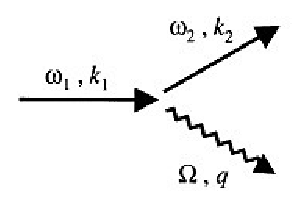
\includegraphics[width=20mm]{109.eps}\label{fig:10.9}\\[\intextsep]
An inelastic light scattering process. The straight arrows represent photons, while the wiggly arrow represents the phonon. The process shown corresponds to Stokes scattering in which the photon is shifted to lower frequency.
\end{minipage}}

Inelastic light scattering can be subdivided into two generic types:
\begin{itemize}
  \item \textbf{Stokes scattering;}
  \item \textbf{Anti-Stokes scattering.}
\end{itemize}
Stokes scattering corresponds to the emission of a phonon (or some other type of material excitation), while anti-Stokes scattering corresponds to phonon absorption. The interaction shown in Fig. \ref{fig:10.9} is thus a Stokes process. Conservation of energy during the interaction requires that:
\begin{equation}\label{equa:10.28}
  \omega_1=\omega_2\pm\Omega
\end{equation}
while conservation of momentum gives:
\begin{equation}\label{equa:10.29}
  \mathbf{k_1}=\mathbf{k_2}\pm\mathbf{q}
\end{equation}
The $+$ signs in eqns \ref{equa:10.28} and \ref{equa:10.29} correspond to phonon emission (Stokes scattering), while the $-$ signs correspond to phonon absorption (anti-Stokes scattering). Thus the light is shifted down in frequency during a Stokes process, and up in frequency in an anti-Stokes event.

Anti-Stokes scattering will only be possible if there are phonons present in the material before the light is incident. The probability for anti-Stokes scattering therefore decreases on lowering the temperature as the phonon populations decrease. This means that the probability for anti-Stokes scattering from optical phonons is very low at cryogenic temperatures. On the other hand, Stokes scattering does not require a phonon to be present and can therefore occur at any temperature. The full quantum mechanical treatment shows that the ratio of anti-Stokes to Stokes scattering events is given by:
\begin{equation}\label{equa:10.30}
  \frac{I_{anti-Stokes}}{I_{Stokes}}=\exp(-\hbar\Omega/k_BT)
\end{equation}
This will be the ratio of the intensities of the anti-Stokes and Stokes lines observed in the Raman or Brillouin spectra.

The frequencies of the phonons involved can be deduced from the frequency shift of the scattered light using eqn \ref{equa:10.28}. Thus the main use of inelastic light scattering is to measure phonon frequencies. This means that inelastic light scattering can give complementary information to that obtained from the infrared spectra. For example, infrared reflectivity measurements tell us nothing about the acoustic phonons, but we can measure the frequencies of some of the acoustic modes using Brillouin scattering experiments. We will consider this complementarity in more detail when we discuss the selection rules for Raman scattering in subsection 10.5.2 below.

The maximum phonon frequency in a typical crystal is about $10^{12} -10^{13}$ Hz. This is almost two orders of magnitude smaller than the frequency of a photon in the visible spectral region. Equation \ref{equa:10.28} therefore tells us that the maximum frequency shift for the photon will be around $1\%$. The wave vector of the photon is directly proportional to its frequency, and we can therefore make the approximation:
\begin{equation}\label{equa:10.31}
  |\mathbf{k}_2|\approx|\mathbf{k}_1|=\frac{n\omega}{c}
\end{equation}
where $n$ is the refractive index of the crystal and $\omega$ is the angular frequency of the incoming light.

We know from eqn \ref{equa:10.29} that $|\mathbf{q}|=|\mathbf{k}_1-\mathbf{k}_2|$. The maximum possible value of $|\mathbf{q}|$ thus occurs for the \textbf{back-scattering geometry} in which the outgoing photon is emitted in the direction back towards the source. In this case, we have:
\begin{equation}\label{equa:10.32}
  q\approx|\mathbf{k}-(-\mathbf{k})|\approx2\frac{n\omega}{c}
\end{equation}
By inserting typical values into eqn \ref{equa:10.32}, we conclude that the maximum value of q that can be accessed in an inelastic light scattering experiment is of order $10^7 \mathrm{m^{-1}}$. This is very small compared to the size of the Brillouin zone in a typical crystal ($\sim10^{10}\mathrm{m^{-1}}$). Inelastic light scattering is thus only able to probe small wave vector phonons.

Raman and Brillouin scattering are generally weak processes, and we therefore expect that the scattering rate will be small. This is because we are dealing with a higher order interaction than for linear interactions such as absorption. Figure \ref{fig:10.9} shows us that three particles are present in the Feynman diagram for inelastic light scattering rather than the two for absorption (see Fig. \ref{fig:10.1}). Therefore, a higher order perturbation term must be involved. This means that we usually have to employ very sensitive detectors to observe the signals even when using a powerful laser beam as the excitation source.

\subsection{Raman scattering}
C. V. Raman was awarded the Nobel prize in 1930 for his discovery of inelastic light scattering from molecules. The process which now carries his name refers to scattering from high frequency excitations such as the vibrational modes of molecules. In the present context of phonon physics, it refers specifically to inelastic light scattering from optical phonons.

Optical phonons are essentially dispersionless near $q = 0$. We argued above that inelastic light scattering can only probe the phonon modes with $q\approx0$. Therefore, Raman scattering gives little information about the dispersion of optical phonons, and its main use is to determine the frequencies of the LO and TO modes near the Brillouin zone centre. For example, when Raman techniques are used to measure polariton dispersion curves (see Section 10.3, and especially Fig. \ref{fig:10.7}), we are only probing a very small portion of the Brillouin zone near $q = 0$.

The complementarity of infrared reflectivity and inelastic light scattering measurements become more apparent when we consider the selection rules for deciding whether a particular optical phonon is Raman active or not. These rules are not the same as those for determining whether the mode is IR active. The full treatment requires the use of group theory. However, a simple rule can be given for crystals that possess inversion symmetry. In these centro symmetric crystals, the vibrational modes must either have even or odd parity under inversion. The odd parity modes are IR active, while the even parity modes are Raman active. Thus the Raman active modes are not IR active, and vice versa. This is called the \textbf{rule of mutual exclusion}, and is a well-known result in molecular physics. In non-centrosymmetric crystals, some modes may be simultaneously IR and Raman active.

As an example of these rules, we can compare silicon and GaAs. Silicon has the diamond structure with inversion symmetry, while GaAs has the non-centrosymmetric zinc blende structure. The TO modes of silicon are not IR ctive, but they are Raman active, while the TO modes of GaAs are both Raman and IR active.

The observation of a Raman spectrum requires specialized apparatus to overcome the difficulties that are inherent to the technique. We pointed out above that the signal is relatively weak, which means that we have to use an intense source such as a laser to produce a sizeable scattering rate. However, the frequency shift of the scattered photons is quite small. We thus need to resolve a weak Raman signal which is very close in wavelength to the elastically scattered light from the laser.

Figure \ref{fig:10.10} shows a basic experimental arrangement that can be used to measure Raman spectra. The sample is excited with a suitable laser, and the scattered light is collected and focussed onto the entrance slit of a scanning spectrometer. The number of photons emitted at a particular wavelength is registered using a photon-counting detector and then the results are stored on a computer for analysis. Photomultiplier tubes have traditionally been employed as the detector in this application, but modem arrangements now tend to use array detectors made with charge coupled devices (CCD arrays). By orientating the sample appropriately, the reflected laser light can be arranged to miss the collection optics. However, this still does not prevent a large number of elastically scattered laser photons entering the spectrometer, and this could potentially saturate the detector. To get around this problem, a high resolution spectrometer with good stray light rejection characteristics is used.

Figure 10.11 shows the Raman spectrum obtained from four III-V crystals at 300 K. The laser source was a Nd:YAG laser operating at $1.06\um$, and a double monochromator with a photomultiplier tube were used to detect the signal. Two strong lines are observed for each crystal. These correspond to the Stokes-shifted signals from the TO phonons and LO phonons, with the LO phonons at the higher frequency. The values obtained from this data agree very well with those deduced from infrared reflectivity measurements. (See Exercise 10.13.)

\subsection{Brillouin scattering}
L. Brillouin gave a theoretical discussion of the scattering of light by acoustic waves in 1922. The technique named after him now refers to inelastic light scattering from acoustic phonons. Its main purpose is to determine the dispersion of these acoustic modes.

The frequency shift of the photons in a Brillouin scattering experiment is given by (see Exercise 10. 14):
\begin{equation}\label{equa:10.33}
  \delta\omega=v_s\frac{2n\omega}{c}\sin{\frac{\theta}{2}}
\end{equation}
where $\omega$ is the angular frequency of the incident light, $n$ is the refractive index of the crystal, $v_s$ is the velocity of the acoustic waves, and $\theta$ is the angle through which the light is scattered. Measurements of $\delta\omega$ therefore allow the velocity of the sound waves to be determined if the refractive index is known. The experimental techniques used for Brillouin scattering are more sophisticated than those for Raman scattering due to the need to be able to detect much smaller frequency shifts. Single-mode lasers must be used to ensure that the laser linewidth is sufficiently small, and a scanning Fabry-Perot interferometer is used instead of a grating spectrometer to obtain the required frequency resolution.

\section{Phonon lifetimes}
The discussion of the phonon modes as classical oscillators in Section 10.2 led us to introduce a phenomenological damping constant $\gamma$. This damping term is needed to explain why the reflectivity in the restrahlen band is less than unity. Analysis of the experimental data led us to conclude that $\gamma$ is typically in the range $10^{11} -10^{12}\mathrm{s^{-1}}$. This very rapid damping is a consequence of the finite lifetime $\tau$ of the optical phonons. Since $\gamma$ is equal to $\tau^{-1}$, the data implies that $\tau$ is in the range 1-10 ps.

\marginnote{
\begin{minipage}{\textwidth}
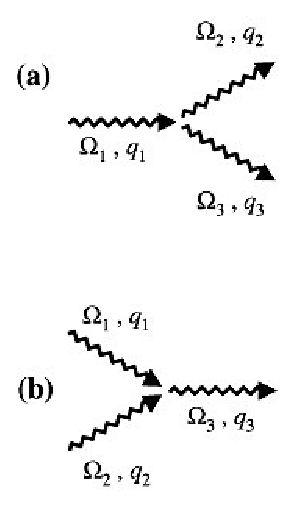
\includegraphics[width=20mm]{1012.eps}\label{fig:10.12}\\[\intextsep]
Three phonon interaction processes. Each wiggly arrow represents a phonon. These processes are caused by an-harmonicity in the crystal.
\end{minipage}}

The very short lifetime of the optical phonons is caused by \textbf{anharmonicity} in the crystal. Phonon modes are solutions of the equations of motion with the assumption that the vibrating atoms are bound in a harmonic potential well. In reality, this is only an approximation that is valid for small displacements. In general, the atoms sit in a potential well of the form:
\begin{equation}\label{equa:10.34}
  U(x)=C_2x^2+C_3x^3+C_4x^4+\cdots
\end{equation}
An example of how interatomic interactions lead to a potential of this form is considered in Exercise 10.15.

The term in $x^2$ in eqn \ref{equa:10.34} is the harmonic term. This leads to simple harmonic oscillator equations of motion with a restoring force $-dU /dx$ proportional to $-x$. The terms in $x^3$ and higher are the \textbf{anharmonic} terms. These anharmonic terms allow phonon-phonon scattering processes. For example, the term in $x^3$ allows interactions involving three phonons. Figure \ref{fig:10.12} illustrates two possible permutations for a three-phonon process.

Figure 10.12(a) shows a three-phonon interaction in which one phonon is annihilated and two new phonons are created. This type of anharmonic interaction is responsible for the fast decay of the optical phonons. We can see why this is so by referring to the generic phonon dispersion curve for the first Brillouin zone shown in Fig. \ref{fig:10.13}. Lattice absorption or Raman scattering creates optical phonons with $q\approx0$. Three-phonon processes allow these phonons to decay into two acoustic phonons as indicated in Fig. \ref{fig:10.13}. Momentum and energy can be conserved if the two acoustic phonons have opposite wave vectors, and their frequency is half that of the optical phonon. With more complex dispersion relationships, and also the possibility for higher order processes, many other types of decay can contribute to the short lifetime of the optical phonons.

The lifetime of the optical phonons can be deduced from Raman data in two different ways. Firstly, the spectral width of the Raman line is affected by lifetime broadening. Provided that other sources of broadening are smaller, the linewidth in frequency units is expected to be $(2\pi\tau)^{-1}$. Thus measurements of the linewidth give a value for $\tau$ independently of the reflectivity data. Secondly, $\tau$ can be measured directly by time-resolved Raman spectroscopy using short pulse lasers. The lifetime of the LO phonons in GaAs has been determined in this way to be 7 ps at 77 K. This value agrees with the linewidth measured in the conventional Raman spectrum. It is also similar to the lifetime of the TO phonons deduced from reflectivity measurements.

\section*{Chapter Summary}
\definecolor{shadecolor}{rgb}{1,0.9,0.9}
\begin{shaded}
\begin{itemize}
  \item The TO phonon modes of polar solids. couple strongly to photons when their frequencies and wave vectors match. Acoustic phonons and LO phonons do not couple directly to light waves.
  \item The interaction between the light and the TO phonon can be modelled by using the classical oscillator model. This model explains why the reflectivity of a polar solid is very high for frequencies in the restrahlen band between $\nu_{TO}$ and $\nu_{LO}$·
  \item The reflectivity in the restrahlen band is $100\%$ for an undamped system, but· damping due to the finite phonon lifetime reduces the reflectivity in real crystals.
  \item The frequencies of the TO. and LO phonon modes are related to each other by the Lyddane-Sachs-Teller relationship given in eqn 10.15.
  \item The lattice absorbs strongly at the TO phonon frequency. The absorption can be measured directly in thin film samples.
  \item The strongly coupled phonon-photon waves at frequencies near the restrahlen band are described as polariton modes.
  \item The electron-phonon coupling in polar crystals leads to polaron effects. Polarons are charge carriers surrounded by a local lattice distortion. The phonon cloud around the electron or hole increases its mass. Polaronic effects are strong in ionic crystals like the alkali halides.
  \item Raman and Brillouin scattering are inelastic light scattering processes from optical and acoustic phonons respectively. Energy and momentum must be conserved in the scattering process.
  \item Stokes and anti-Stokes inelastic light scattering processes correspond to phonon emission and absorption. respectively. AntiStokes scattering front optical phonons is very improbable at low temperatures.
  \item Optical phonons have short lifetimes due to the possibility of decay into two acoustic phcmons by anharmonic interactions.

\end{itemize}
\end{shaded}
\section*{Further Reading}
Introductory reading on phonons may be found in practically any solid state physics text, for example: Ashcroft and Mermin (1976), Bums (1985), Ibach and Luth (1995) or Kittel (1996).

The theory of polaritons and polarons is described in more detail in Madelung (1978). Pidgeon (1980) and Seeger (1997) discuss cyclotron resonance experiments in detail. The properties of self-trapped excitons are covered by Song and Williams (1993), while Pope and Swenberg (1999) discuss polaronic hopping transport, especially in organic semiconductors.

A classic text on the infrared physics of molecules and solids is Houghton and Smith (1966). The techniques of inelastic light scattering are described in detail by Mooradian (1972) or Yu and Cardona (1996). The study of phonon dynamics by ultra-fast laser techniques is described by Shah (1999).

\chapter{Nonlinear Optic}\label{chap:11}






\end{document}  